% AVA Internal Report #1 — FLOYDS Pipeline Recalibration for Reverberation Mapping
\documentclass[10pt,a4paper,oneside]{report}
\usepackage[T1]{fontenc}
\usepackage[a4paper,top=2.3cm,bottom=2.5cm,left=2.4cm,right=2.4cm,headsep=0.6cm]{geometry}
\usepackage{graphicx}
\usepackage{pifont}
\usepackage{amsmath}
\usepackage{amssymb}
\usepackage{tabularx}
\usepackage[round,authoryear]{natbib}
\usepackage[font=small,labelfont=bf,labelsep=period,justification=justified,singlelinecheck=false]{caption}
\usepackage{tikz}
\usetikzlibrary{positioning,arrows.meta,shapes.misc,fit,calc}

%% AVA brand identity — all colours, fonts, headings, boxes, page style
\usepackage{ava_style}
\colorlet{mnrasblue}{avaInkBlue}

%% Override header right side for this document
\renewcommand{\AVAManualTitle}{FLOYDS Pipeline Report}

%% Restore chapter-level heading format (ava_style uses sections; report class has chapters)
\usepackage{titlesec}
\titleformat{\chapter}[block]
  {\normalfont\large\bfseries\color{avaInkBlue}}{\thechapter}{1em}{\MakeUppercase}
\titlespacing*{\chapter}{0pt}{0pt}{14pt}
\titleformat{\section}
  {\normalfont\normalsize\bfseries\color{avaInkBlue}}{{\thesection}}{1em}{\MakeUppercase}[\color{avaInkBlue}\titlerule]
\titleformat{\subsection}{\normalfont\normalsize\bfseries\color{avaInkBlue}}{\thesubsection}{1em}{}
\titleformat{\subsubsection}[runin]{\normalfont\normalsize\itshape\color{avaInkBlue}}{\thesubsubsection}{0.6em}{}[.]
\titlespacing*{\section}{0pt}{12pt}{5pt}
\titlespacing*{\subsection}{0pt}{9pt}{3pt}

%% Convenience macros
\newcommand{\banzai}{\textsc{banzai-floyds}}
\newcommand{\kms}{km\,s$^{-1}$}

\graphicspath{{figures/}}
% generated by work/scripts/gen_numbers.py -- do not edit
\newcommand{\OIIIbOld}{$-168\pm160$ (50)}
\newcommand{\OIIIbNew}{$-253\pm25$ (50)}
\newcommand{\OIIIrOld}{$-456\pm344$ (39)}
\newcommand{\OIIIrNew}{$-242\pm40$ (50)}
\newcommand{\OIIIfourOld}{$-196\pm187$ (49)}
\newcommand{\OIIIfourNew}{$-285\pm26$ (48)}
\newcommand{\NeIIIOld}{$-157\pm238$ (46)}
\newcommand{\NeIIINew}{$-154\pm90$ (47)}
\newcommand{\OIOld}{--}
\newcommand{\OINew}{$-169\pm58$ (29)}
\newcommand{\CaKOld}{$+4\pm81$ (47)}
\newcommand{\CaKNew}{$+26\pm83$ (48)}
\newcommand{\OIN}{29}
\newcommand{\OIvel}{$-169$}
\newcommand{\OIIIvel}{$-253$}
\newcommand{\FrOld}{13.7}
\newcommand{\FrMedOld}{11.8}
\newcommand{\SpOld}{6/121}
\newcommand{\FrNewOpt}{2.6}
\newcommand{\FrMedNewOpt}{3.4}
\newcommand{\SpNewOpt}{3/6}
\newcommand{\FrNewBox}{2.6}
\newcommand{\FrMedNewBox}{3.5}
\newcommand{\SpNewBox}{3/7}
\newcommand{\SpMaxOld}{121}
\newcommand{\SpMaxNew}{6}
\newcommand{\SSbaOld}{1.61}
\newcommand{\SSbaOpt}{1.44}
\newcommand{\SSbaBox}{1.51}
\newcommand{\SSbbOld}{1.84}
\newcommand{\SSbbOpt}{1.64}
\newcommand{\SSbbBox}{1.66}
\newcommand{\SSbcOld}{2.00}
\newcommand{\SSbcOpt}{1.82}
\newcommand{\SSbcBox}{1.89}
\newcommand{\SSbdOld}{2.78}
\newcommand{\SSbdOpt}{2.60}
\newcommand{\SSbdBox}{2.72}
\newcommand{\SSraOld}{2.08}
\newcommand{\SSraOpt}{1.09}
\newcommand{\SSraBox}{1.09}
\newcommand{\SSrbOld}{1.37}
\newcommand{\SSrbOpt}{1.01}
\newcommand{\SSrbBox}{1.02}
\newcommand{\SSrcOld}{3.18}
\newcommand{\SSrcOpt}{1.65}
\newcommand{\SSrcBox}{1.68}
\newcommand{\SSrdOld}{7.68}
\newcommand{\SSrdOpt}{2.17}
\newcommand{\SSrdBox}{2.13}
\newcommand{\SSreOld}{12.74}
\newcommand{\SSreOpt}{3.68}
\newcommand{\SSreBox}{3.52}
\newcommand{\FOIIIbOld}{12.7}
\newcommand{\FOIIIrOld}{27.6}
\newcommand{\FRBOld}{29.2}
\newcommand{\FOIIIbOpt}{8.8}
\newcommand{\FOIIIrOpt}{10.5}
\newcommand{\FRBOpt}{9.7}
\newcommand{\FOIIIbBox}{9.3}
\newcommand{\FOIIIrBox}{8.9}
\newcommand{\FRBBox}{8.8}
\newcommand{\CLbOld}{1.4}
\newcommand{\CLbNew}{1.2}
\newcommand{\CLrOld}{1.9}
\newcommand{\CLrNew}{1.8}
\newcommand{\EGfrOld}{10.6}
\newcommand{\EGfrNew}{2.8}
\newcommand{\FringeResidualStd}{3}
\newcommand{\AmpSixA}{5.39$^{a}$}
\newcommand{\AmpSixB}{$5.39\pm0.83$}
\newcommand{\AmpSixC}{$1.97\pm0.18$}
\newcommand{\AmpSixD}{$1.17\pm0.13$}
\newcommand{\AmpTwoA}{7.29$^{a}$}
\newcommand{\AmpTwoB}{$7.29\pm0.58$}
\newcommand{\AmpTwoC}{$2.35\pm0.05$}
\newcommand{\AmpTwoD}{$1.30\pm0.13$}
\newcommand{\FVnoneF}{16.0}
\newcommand{\FVampF}{6.0}
\newcommand{\FVstdF}{5.6}
\newcommand{\FVensF}{6.4}
\newcommand{\FVharmF}{3.5}
\newcommand{\FVflatF}{3.7}
\newcommand{\FVnoiseF}{1.9}
\newcommand{\FVnoneE}{18.9}
\newcommand{\FVampE}{7.2}
\newcommand{\FVstdE}{--}
\newcommand{\FVensE}{3.7}
\newcommand{\FVharmE}{3.4}
\newcommand{\FVflatE}{3.5}
\newcommand{\FVnoiseE}{1.4}
\newcommand{\IndivOldF}{17}
\newcommand{\IndivNewF}{4.9}
\newcommand{\IndivOldE}{12}
\newcommand{\IndivNewE}{4.2}


\begin{document}

%% ---- Title page via ava_style \avatitlepage --------------------------
%% Args: {Title}{Version}{Date}{Author}{Email}{Address}
\avatitlepage
  {Wavelength, trace, fringe, extraction and flux recalibration\\
   of LCO FLOYDS spectra for reverberation mapping\\[4pt]
   {\normalsize\upshape Diagnosis of \banzai~1.0.1
    and target-independent corrections}}
  {1.0}
  {November 2026}
  {Juan V.\ Hern\'andez Santisteban}
  {jvhs1@st-andrews.ac.uk}
  {School of Physics and Astronomy, University of St Andrews,
   North Haugh, St Andrews, KY16~9SS, UK}

%% ---- Abstract page --------------------------------------------------
\begin{titlepage}
\vspace*{2cm}
{\large\bfseries\color{avaInkBlue} Abstract\par}
\vspace{0.6em}
We diagnose the LCO FLOYDS pipeline \banzai{} for reverberation mapping (RM), using a Fairall~9 campaign at Siding
Spring (COJ; 100 spectra through the 6\,arcsec slit, 57 standard-star spectra, 122 arcs) and an NGC\,4151 campaign at
Haleakal\=a (OGG; 60 spectra, 100 standard-star spectra), and we describe target-independent corrections, now built into
\banzai{} and run from the raw frames. Our final version (improved v3) addresses every problem we found.
(i) \textit{Wavelengths}: the arc fit leaves H$\beta$/[O\,{\sc iii}] and H$\alpha$ unconstrained (the archive red order
is off by $-8$\,\AA{} at Hg\,4916) and a compact object's zero point in a wide slit depends on its position across the
slit (up to $\pm2''$, i.e.\ $\pm17$\,\AA{} for NGC\,4151). Adding the detected but unused lines to the arc fit and
measuring the object's zero point from the telluric bands in its own light bring the [O\,{\sc iii}] scatter from
exposure to exposure to 0.5--0.9\,\AA{} and the two orders into agreement to 0.3\,\AA{} (COJ). (ii)
\textit{Fringing}: the archive frames are divided by an eight-month-old lamp flat shifted along the slit by up to
hundreds of pixels, which destroys data in 13 of 50 frames and biases the flux by up to $\pm10$ per cent; a lamp flat
gives the phase of the fringes but not their shape. A two-harmonic fringe model with the lamp phase, fitted to each
extracted spectrum jointly with a telluric template, reduces the red-order fringing of Fairall~9 from 13.7 (archive)
and 8.1 (\banzai{}~1.1.0) to 1.9 per cent. (iii) \textit{Telluric and flux calibration}: standards are selected by
proposal rather than slit width, several nightly standards are missing from the catalogue, a single standard
transfers its clouds and its noise to the science, and the archive spectra are twice too bright because 1.0.1 does not
scale by the exposure time. An ensemble of the nine nearest standards with the grey level of the clearest half, a
telluric correction confined to the absorption bands and two added standards reduce the scatter of the red/blue
[O\,{\sc iii}] flux ratio from 29.2 (archive) and 8.9 (1.1.0) to 6.9 per cent, and bridge a factor-1.8 throughput change
of the OGG telescope. (iv) \textit{Traces}: a physical model of the object trace (refraction plus an instrumental
shape for each site) keeps the faint ends of the orders at 0.1--0.3\,px where the polynomial fails. The uncertainties
are correct per pixel at both sites. We list the open issues and give recommendations for observing and for the
pipeline.

\vfill
{\small\color{avaInkBlue!70}%
  Keywords: techniques: spectroscopic ---
  methods: data analysis ---
  instrumentation: spectrographs ---
  galaxies: Seyfert}
\end{titlepage}

\tableofcontents
\clearpage

\chapter*{Executive summary}
\addcontentsline{toc}{chapter}{Executive summary}
\label{sec:exec}

\textit{What this report is.} We examined every step of \banzai{}, the LCO pipeline for the FLOYDS spectrographs,
that matters for reverberation mapping (RM). We tested the archive products (\banzai{} version 1.0.1) and the current
release (1.1.0) on a Fairall~9 campaign at Siding Spring (COJ) and an NGC\,4151 campaign at Haleakal\=a (OGG). For each step we show what the pipeline
does, where and why it fails, what we changed, and what the change achieves. All corrections are target-independent
(no knowledge of the science target is used) and are built into \banzai{} (branch \texttt{rm-improvements} of
\url{https://github.com/Alymantara/banzai-floyds}); a whole data set is reduced from the raw frames with one command
(Appendix~\ref{sec:app_install}).

\textit{Status.} \textbf{Improved v3 is our final version for now.} It reduces all 833 raw frames of the two
campaigns without failures, and we verified it step by step at both sites (Chapter~\ref{sec:sites}). Table~\ref{tab:exec_numbers}
gives the headline numbers and Table~\ref{tab:exec_issues} lists every problem we found, what v3 does about it and where
in the report it is explained. We then inspected the worst
v3 reductions and found problems in two steps we had not examined: the cosmic-ray detector and the sky model under the
object (issues 27--31, Chapter~\ref{sec:cosmics}). The fixes are in the code and verified on a sample, but the
products have not yet been re-reduced with them. Every product now carries header keywords that record the quality of
its reduction, and a flag bitmask (Section~\ref{sec:qc}). The reductions compared are defined in
Table~\ref{tab:versions_names}, and the terms used throughout (orders, visits, pulls, fringe measures) in the
Conventions (p.~\pageref{sec:conventions}).

\begin{table}[!htbp]
\centering
\caption{Headline numbers. Fairall~9 at COJ and NGC\,4151 at OGG, 6\,arcsec slit. Scatters are robust rms (see
Conventions) over all exposures. ``1.1.0 as released'' is \banzai{}~1.1.0 run from raw without the object wavelength
zero point of this work (elsewhere in the report the 1.1.0 run includes it; Table~\ref{tab:versions_names}).}
\label{tab:exec_numbers}
\small
\begin{tabular}{@{}>{\raggedright\arraybackslash}p{5.6cm}cccc@{}}
\toprule
Quantity (unit) & \banzai{}~1.0.1 & \banzai{}~1.1.0 & \multicolumn{2}{c}{improved v3 (final)} \\
 & (archive) & as released & COJ & OGG \\
\midrule
{[O\,{\sc iii}]} wavelength scatter, red / blue order (\AA) & 6.4 / 2.8 & 6.6 / 3.1 & 0.69 / 0.45 & 0.94 / 0.53 \\
{[O\,{\sc iii}]} wavelength, red $-$ blue order (\AA) & $-5.9\pm3.0$ & $+0.4\pm3.1$ & $+0.30\pm0.79$ & $+1.39\pm0.88$ \\
Red-order fringe residual, rms (per cent) & 13.7 & 8.1 & 1.9 & 2.5$^{a}$ \\
Residual in the water band 8130--8360\,\AA, rms (per cent) & 16.1 & 8.0 & 3.2 & 2.7 \\
Red/blue [O\,{\sc iii}] flux ratio scatter (per cent) & 29.2 & 8.9 & 6.9 & 6.2 \\
Uncertainties: rms of the pull, red order (1 = correct errors) & 1.7--2.2$^{b}$ & up to 1.6 & 0.94--1.06 & 0.98--1.27 \\
Absolute flux level (factor) & $\times2.2$ too bright & correct & correct & correct$^{c}$ \\
\bottomrule
\end{tabular}
\par\smallskip\raggedright\footnotesize
$^{a}$Includes NGC\,4151's own lines, which fall in the measurement windows. The difference between the two
exposures of a visit, which removes all structure common to both, is the same as at COJ (0.66--0.69 per cent).
$^{b}$Beyond 7700\,\AA. $^{c}$Also across a factor-1.8 change in telescope throughput, thanks to two added standards
(Section~\ref{sec:sites_flux}). All absolute levels are biased high by the slit losses of the 2\,arcsec standards; the
usual RM scaling of each spectrum to the [O\,{\sc iii}] flux removes this bias.
\end{table}

\textit{The issues.} In Table~\ref{tab:exec_issues}, ``1.0.1'' marks problems of the archive products and ``1.1.0''
problems that remain in the current release. Issues are grouped by pipeline step, so their numbers are not in order. Status: \textit{solved} (fixed in v3 and verified), \textit{mitigated}
(reduced or flagged, not removed), \textit{open} (not addressed in the software), \textit{operations} (needs a change in
how data are taken). The open items and recommendations for LCO are collected in Chapter~\ref{sec:recommendations}.

{\small
\setlength{\LTcapwidth}{\textwidth}
\begin{longtable}{@{}>{\raggedright\arraybackslash}p{0.3cm}>{\raggedright\arraybackslash}p{5.4cm}>{\raggedright\arraybackslash}p{5.3cm}>{\raggedright\arraybackslash}p{1.6cm}>{\raggedright\arraybackslash}p{1.9cm}@{}}
\caption{Problems found, what the final pipeline (improved v3) does about them, and where in this report.}
\label{tab:exec_issues}\\
\toprule
\# & Problem and its effect & What v3 does & Where & Status \\
\midrule
\endfirsthead
\toprule
\# & Problem and its effect & What v3 does & Where & Status \\
\midrule
\endhead
\bottomrule
\endfoot
\multicolumn{5}{@{}l}{\textit{Wavelength calibration}}\\
1 & The arc fit uses no line between Hg\,4358 and 5461\,\AA{} (blue) and none blueward of 5461 or between 5791 and
6965\,\AA{} (red): H$\beta$/[O\,{\sc iii}] and H$\alpha$ are interpolated or extrapolated. 1.0.1: red order off by
$-8$\,\AA{} at Hg\,4916; 1.1.0: up to 0.6\,\AA. & Hg\,4916 and Ar\,6416, 6677, 6753, 6767, detected in every arc,
added to the arc fit with measured strengths; error at Hg\,4916 $\approx0.1$\,\AA, orders agree to 0.3\,\AA. &
\S\ref{sec:wl_lines}, \S\ref{sec:sites_arcs} & solved \\
2 & The Zn lamp is ``on'' in the headers but no Zn line is detected; Zn would fill the blue gap. & -- &
\S\ref{sec:wl_lines} & operations \\
3 & No per-exposure zero point for the object (1.0.1, 1.1.0): in a 6\,arcsec slit the object's position across the
slit shifts its spectrum by $\approx10$\,\AA{} per arcsec, which arcs and sky lines cannot measure. [O\,{\sc iii}]
scatters by 3--7\,\AA{} between exposures, up to $\pm17$\,\AA{} for NGC\,4151. & Zero point measured from the telluric
bands in the object's own light, transferred to the blue order: scatter 0.5--0.9\,\AA. & \S\ref{sec:wl_zp},
\S\ref{sec:sites_zp} & solved \\
4 & The absolute wavelength zero point is that of the telluric template, uncertain by $\approx\pm2$--4\,\AA. & Nothing:
it is a constant offset and does not affect the agreement between exposures or between orders. & \S\ref{sec:wl_zp} & open (harmless for RM) \\
\midrule
\multicolumn{5}{@{}l}{\textit{Order and object traces}}\\
5 & The object trace is a polynomial (1.0.1, 1.1.0): at the faint red end it is off by 0.8--1.4\,px (1--2 per cent
flux loss), and much worse for targets 30--60 times fainter than Fairall~9. & Physical model (atmospheric refraction along the
slit + an instrumental shape for each site + a small smooth correction fitted to the residuals): 0.1--0.3\,px down to 60 times fainter; templates for COJ and OGG.
& \S\ref{sec:traces_object}, \S\ref{sec:traces_model}, \S\ref{sec:sites_trace} & solved \\
6 & The position of the orders on the detector in each frame is fitted on the light of the science target, which
fails for faint targets. For the targets here it agrees with the lamp flat to 0.14\,px. & Unchanged (the 1.1.0 fit).
The lamp flat of the same block would measure it at a signal-to-noise ratio of thousands. & \S\ref{sec:traces_orders} & open (faint targets) \\
7 & The shapes of the orders on the detector come only from the sky flats in a list fixed in the code; for OGG the
newest are from 2019. & Sky flats already processed by the LCO archive can also be used; the 2019 OGG set works for
2024--25 data. & \S\ref{sec:traces_orders}, \S\ref{sec:sites_data} &
mitigated \\
\midrule
\multicolumn{5}{@{}l}{\textit{Fringing and extraction}}\\
8 & 1.0.1 divides every frame by a whole eight-month-old lamp flat, including its slit illumination: flux biased by up
to $\pm10$ per cent, wavelength and frame dependent. & No 2-d division by a lamp flat. & \S\ref{sec:fringe_banzai} &
solved \\
9 & 1.0.1 shifts that flat along the slit by up to hundreds of pixels (the fit locks on to wrong
matches of the repeating fringe pattern); the invalid edge of the shifted flat destroys data in 13 of 50 frames
(spikes, striped sky). & As 8; the destroyed pixels are never created. & \S\ref{sec:fringe_banzai},
\S\ref{sec:traces_object} & solved \\
10 & A lamp flat gives the phase of the fringes but not their amplitude or shape (the slit-filling lamp smooths them
differently from a point source), so scaling a lamp pattern leaves spiky residuals. & A two-harmonic fringe model with
the lamp phase, fitted to each extracted spectrum. & \S\ref{sec:fringe_harmonic} & solved \\
11 & 1.1.0 still leaves 8 per cent rms of fringing (Fairall~9). & 1.9 per cent (EG\,21: 1.5). & \S\ref{sec:raw_compare} &
solved \\
12 & Residual fringes at 6500--7500\,\AA: the phase of a single 6\,arcsec lamp flat is noisy there and slow structure
in the lamp pattern dominates it. & Phase from a phase master (median of the lamp flats of 1--2
months) after a high-pass filter; the model starts at 6200\,\AA{} and its amplitude and phase may change every
200\,\AA. & \S\ref{sec:fringe_pipeline}, \S\ref{sec:fringe_joint} & solved \\
13 & Fringes inside the telluric bands were not fitted but interpolated across. This left a 4 per cent residual in
the transmission measured on the standards, and so in every science spectrum. A 0.7 per cent residual that is fixed on
the detector also remained. & Fringes fitted jointly with a telluric template; a template of the fixed residual is
measured on the standards for each slit and removed. &
\S\ref{sec:fringe_joint} & solved \\
\midrule
\multicolumn{5}{@{}l}{\textit{Telluric correction}}\\
14 & 1.1.0 divides almost the whole red order by the standard's observed/expected ratio, so the standard's noise and
residuals (1--3 per cent) appear in every science spectrum. The transmission of a single standard is noisy. &
Transmission applied only inside the absorption bands (between the points where the absorption is 1 per cent deep),
median of the nine nearest standards. &
\S\ref{sec:flux_tell} & solved \\
15 & The saturated O$_2$ A band leaves $\pm20$ per cent residuals in 6\,arcsec spectra, because the 2\,arcsec standards
resolve it differently. The sky lines fill the slit, so they cannot give the resolution of the object's spectrum. &
Flagged in science spectra (bit 2 of the mask, 7580--7700\,\AA); smoothing the standards' transmission to match gave
no real gain. & \S\ref{sec:flux_tell} & mitigated \\
16 & The water absorption changes from night to night ($\approx3.5$ per cent in the band level); a median of standards
does not follow it. & -- & \S\ref{sec:raw_compare}, \S\ref{sec:recommendations} & open \\
17 & Beyond 8900\,\AA{} there is no telluric-free continuum: the transmission and the sensitivity are extrapolated
there (a step of $\approx30$ per cent near 9285\,\AA{} in every version). & Water band included in the telluric bands
(8900--9900\,\AA); the red end should still be used with care. & App.~\ref{sec:app_v1}, \S\ref{sec:recommendations} & open \\
\midrule
\multicolumn{5}{@{}l}{\textit{Flux calibration}}\\
18 & 1.0.1 does not scale by the exposure time: 600\,s science calibrated with 300\,s standards is 2.2 times too bright
in the archive. & Fixed in 1.1.0; v3 agrees with 1.1.0 to 4 per cent. & \S\ref{sec:flux_banzai} & solved (1.1.0) \\
19 & Standards are chosen by block or proposal, not slit width, and a single standard transfers its clouds (grey levels
of nine consecutive standards span a factor 2) and noise to the science. The 1.0.1 sensitivity functions contain the
fringes and spikes. & Median of the sensitivities of the nine nearest standards, each first scaled by its grey factor; overall level
from the clearest half; red/blue [O\,{\sc iii}] scatter 29.2 (1.0.1), 8.9 (1.1.0) $\rightarrow$ 6.9 per cent. &
\S\ref{sec:flux_banzai}, \S\ref{sec:flux_ensemble} & solved \\
20 & Nightly standards missing from the catalogue (EG\,21 at COJ; Feige\,67 and GD\,153 at OGG) are reduced as science and
never calibrate anything. & Feige\,67 and GD\,153 added (references from ESO; Feige\,67 extended beyond 9200\,\AA). EG\,21
has only a 50\,\AA{} reference. & \S\ref{sec:flux_model}, \S\ref{sec:sites_flux} & solved for OGG; open for EG\,21 \\
21 & The OGG telescope throughput rose by a factor 1.8 between 2025 April 7 and May 2 (re-aluminisation of the
primary mirror), most in the blue (48 per cent more at 3400\,\AA{} than at 5800\,\AA), and all catalogue standards are
from after it: earlier frames were calibrated 1.8 times too faint ([O\,{\sc iii}] scatter 26 per cent) and up to
30 per cent off in shape. & With the added
standards the two periods agree to 7 per cent ([O\,{\sc iii}] scatter 9.4 per cent). An ensemble must not combine
standards across such a change. & \S\ref{sec:sites_flux}, \S\ref{sec:shape_stability} & solved here; open in general; operations \\
22 & The standards are 2\,arcsec, the RM science 6\,arcsec: absolute levels are biased high by the standards' slit
losses. & Grey level from the clearest standards (lowest bias). RM scaling to [O\,{\sc iii}] removes it. &
\S\ref{sec:flux_banzai} & open (harmless for RM) \\
\midrule
\multicolumn{5}{@{}l}{\textit{Cosmic rays and the sky model} (found after the improved v3 run; Chapter~\ref{sec:cosmics})}\\
27 & The cosmic-ray detector of 1.1.0, LA Cosmic (1.0.1 has none), takes the core of a bright star in good seeing
for cosmic rays: up to 46 per cent of the core of BD$+28^\circ4211$ at OGG, whose spectrum then scatters by 2.9 times
its errors. & LA Cosmic is given a model of the object (7-pixel median along the dispersion) besides the sky; the
flagged share of the core drops from 46 to 0.1 per cent. & \S\ref{sec:cr_stars}, \S\ref{sec:cr_model} & fixed in code; re-reduction pending \\
28 & LA Cosmic clips bright narrow lines that are resolved along the slit, and the extraction scales up what is left:
H$\alpha$ of NGC\,4151 flagged in 7 of 60 frames, 2.64 and 1.18 times too bright in two. [O\,{\sc iii}]\,5007 never
flagged. Can affect any bright emission-line object in good seeing. & Object model (flagged pixels on H$\alpha$ drop from
179 to 15 and from 119 to 0 in those two frames; fluxes within 2 per cent). Wavelength bins that lose more than half of
their profile weight to flags are masked instead of scaled up, and counted in the header. & \S\ref{sec:cr_lines}, \S\ref{sec:cr_guard} & mitigated in code;
re-reduction pending \\
29 & When the object is wide (poor seeing) and the sky bright (Moon), the spline that models the sky gets a knot at
every pixel beside the object and follows the noise. The extracted flux then scatters by 3--4 times its errors (six
Fairall~9 frames), and LA Cosmic flags the object ($\approx240$ false detections per frame). Also in 1.1.0. & A sky
line is only treated as such if it stands out by 5$\sigma$ from the noise of a first-pass sky fit; the scatter drops
from 3.0--3.3 to 1.1--1.2 times the errors. & \S\ref{sec:cr_sky} & fixed in code; re-reduction
pending \\
30 & LA Cosmic (1.1.0) misses real cosmic rays on bright cores and line peaks (66 per cent found above 10$\sigma$; none
of 8 on the core of BD$+28^\circ4211$) and spreads its detections into bright regions. & With the object model, 97 per cent of
artificial cosmic rays added to the frames are found, at the cost of 1--5 more small false detections per frame on
bright traces. After LA Cosmic, the two exposures of each visit are now compared, and a flag is removed when the
partner exposure shows the same structure, which is therefore real (10--22 per cent fewer flagged pixels; on the H$\alpha$ peak
15 to 0 pixels), with no change in the agreement of their fluxes. Standards are single exposures and use the object
model only. & \S\ref{sec:cr_verify}, \S\ref{sec:cr_pair} & fixed in code; re-reduction
pending \\
31 & A warm pixel of the OGG camera at $(x,y)=(1465,409)$ is not in the bad-pixel mask (flagged as a cosmic ray in every
frame, on the wing of [O\,{\sc iii}]\,4959 of NGC\,4151). & -- & \S\ref{sec:cr_lines} & open \\
32 & Nothing in the products records how good a reduction is. & Quality keywords (\texttt{L1Q}) and a flag bitmask
in every product
(added to all 317 products of the final reductions), and a command that tabulates them. & \S\ref{sec:qc} & solved \\
\midrule
\multicolumn{5}{@{}l}{\textit{Uncertainties and products}}\\
23 & Uncertainties: 1.0.1 underestimates the red-order errors by a factor 1.7--2.2 (the fringe residuals are not in
them), 1.1.0 by up to 1.6. & Correct per pixel at both sites (rms of the pull 0.9--1.1; 1.3 at OGG where the signal is
high). Quantities integrated over many pixels need errors $\approx20$--30 per cent larger, because the fringe and
telluric residuals are not in the error array. & \S\ref{sec:raw_errors},
\S\ref{sec:sites_verify} & solved per pixel; documented \\
24 & The combined spectrum of the \texttt{-1d} product mixes the two orders, which are not aligned, over
4540--5760\,\AA. & Use the separate spectrum of each order (\texttt{EXTRACTED} table of the \texttt{-1d} product). & \S\ref{sec:recommendations} & open \\
25 & A processed 2-d frame is 47\,MB, of which 43\,MB is an uncompressed table of all pixels: a decade of data
would not fit on disk. & After a run, the diagnostic images and the pixel table are removed from the 2-d products
($\approx2$\,GB per site and season of $\approx400$ frames). & \S\ref{sec:sites_disk} & mitigated \\
26 & Installation fails on Apple-silicon laptops with an Intel Python or Intel compiler settings. & A native arm64 Python
environment, and a wrapper script that runs the pipeline without the user's compiler settings. & App.~\ref{sec:app_install} & solved \\
\end{longtable}
}

\textit{How to read the rest.} Chapter~\ref{sec:summary} summarises the pipeline and the changes step by step
(Fig.~\ref{fig:flow}, Table~\ref{tab:stages}); Chapter~\ref{sec:intro} introduces the problem and the data;
Chapter~\ref{sec:diagnostics} defines the measurements;
Chapters~\ref{sec:traces}--\ref{sec:flux} treat traces, wavelengths, fringing and flux calibration in turn;
Chapter~\ref{sec:raw} runs the pipeline from raw and compares all versions; Chapter~\ref{sec:sites} describes the final
version and verifies it at both sites; Chapter~\ref{sec:cosmics} treats cosmic rays and the sky model and defines the
quality keywords; Chapter~\ref{sec:recommendations} gives the recommendations.

\chapter{Summary of the pipeline and of the changes}
\label{sec:summary}

\section*{Reductions compared}
Five reductions of the same exposures are compared in this report (Table~\ref{tab:versions_names}): two are
\banzai{} as distributed, the other three successive improved versions of it. These names are used throughout.

\begin{table}[!htbp]
\centering
\caption{The reductions compared in this report.}
\label{tab:versions_names}
\small
\begin{tabular}{@{}lp{11.3cm}@{}}
\toprule
Name & What it is \\
\midrule
\banzai{}~1.0.1 (archive) & The products in the LCO archive. \\
\banzai{}~1.1.0 (stock) & The current release, run here from the raw frames with its default settings, except
that the object wavelength zero point of this work (Section~\ref{sec:wl_zp}) was already applied; without it the
[O\,{\sc iii}] position of Fairall~9 scatters by 6.6\,\AA{} (red order) and 3.1\,\AA{} (blue) between exposures,
instead of 0.6 and 0.4\,\AA. Its fringe, telluric and flux results are those of 1.1.0. \\
Improved v1 & The corrections of Chapters~\ref{sec:traces}--\ref{sec:flux} applied to the archive products
(re-extraction, harmonic fringe model, arc refit, telluric zero point, template$\times$nightly flux
calibration). \\
Improved v2 & The first improved \banzai{} run from raw: harmonic fringe stage (bands masked, onset 6500\,\AA, nodes
every 400\,\AA), combined trace model, telluric correction restricted to the bands and taken from the nine nearest
standards; single-standard flux calibration. \\
\textbf{Improved v3 (final)} & Our final version for now, and the default configuration of the branch: v2 plus the
joint fringe + telluric fit, the residual fringe template of the slit, wider telluric bands, the O$_2$ A band flagged
in science spectra, the ensemble flux calibration, the unused arc lines added to the arc fit, an object-trace template
for each site, and Feige\,67 and GD\,153 as flux standards. Verified at both FLOYDS sites (Chapter~\ref{sec:sites}). \\
\bottomrule
\end{tabular}
\end{table}

\section*{Overview}

This report examines every step of the FLOYDS reduction that matters for reverberation mapping (RM), shows for each
step what the archive pipeline \banzai{}~1.0.1 does, where it fails (with examples from the Fairall~9 campaign), what we
changed, and what the change achieves. The corrections are target-independent: no information about the science
target is used. They were developed on the public \texttt{-1d}/\texttt{-2d} archive files
(Chapters~\ref{sec:traces}--\ref{sec:flux}); the fringe and trace corrections now run inside \banzai{} from the
raw frames, in one pass and with fewer steps than \banzai{}~1.1.0 (stock) (Chapter~\ref{sec:raw}), as do the
telluric correction, the ensemble flux calibration with the grey level from the clearest standards and the added arc
lines. Improved v3 is our final version for now; Chapter~\ref{sec:sites} verifies it on a second campaign taken with
the other FLOYDS (OGG).
Fig.~\ref{fig:flow} shows the chain and Table~\ref{tab:stages} summarises each step. The quality metrics of the
archive products and of the recalibrated spectra are collected in Table~\ref{tab:summary}.



\begin{figure}[!htbp]
\centering
\begin{tikzpicture}[
  node distance=5mm and 7mm,
  box/.style={draw=avaInkBlue, rounded corners=2pt, thick, align=left, font=\small, text width=6.1cm,
              inner sep=4pt, fill=white},
  new/.style={box, fill=blue!6},
  inp/.style={draw=black!45, dashed, rounded corners=2pt, align=left, font=\footnotesize, text width=3.6cm,
              inner sep=3pt, fill=black!3},
  arr/.style={-{Stealth[length=2.2mm]}, thick, avaInkBlue},
  side/.style={-{Stealth[length=1.8mm]}, black!50}]
\node[box] (raw) {\textbf{Raw frames} (science, standards, arcs, lamp flats, sky flats)};
\node[new, below=of raw] (trace) {\textbf{1. Order and object traces} (Ch.~\ref{sec:traces})\\
  order position per block from the same-block lamp flat; object trace checked against the data};
\node[new, below=of trace] (rex) {\textbf{2. Extraction without 2-d fringe division} (Ch.~\ref{sec:fringe})\\
  no flat division; \banzai{} sky model and optimal extraction};
\node[new, below=of rex] (fr1) {\textbf{3. Harmonic fringe fit} (Ch.~\ref{sec:fringe})\\
  phase from lamp-flat master, fitted per spectrum jointly with a telluric template; residual template per slit};
\node[new, below=of fr1] (wl) {\textbf{4. Wavelengths} (Ch.~\ref{sec:wavelength})\\
  arc fit with the added lines; object zero point from the telluric bands};
\node[new, below=of wl] (flux) {\textbf{5. Flux and telluric calibration} (Ch.~\ref{sec:flux})\\
  grey-normalised median of the nine nearest standards (template $\times$ nightly for coarse references)};
\node[new, below=of flux] (fr2) {\textbf{6. Red end of the fringe fit} (Ch.~\ref{sec:fringe})\\
  beyond 8850\,\AA: fit on the telluric-corrected spectrum (one stage in the pipeline)};
\node[box, below=of fr2] (out) {\textbf{Calibrated spectra per order} (red and blue kept separate)};
\foreach \a/\b in {raw/trace, trace/rex, rex/fr1, fr1/wl, wl/flux, flux/fr2, fr2/out} \draw[arr] (\a) -- (\b);
\node[inp, right=of trace] (i1) {sky flats (order shape, one per slit and epoch); same-block lamp flat (position)};
\node[inp, right=of fr1] (i2) {lamp-flat phase master (median over 1--2 months, per slit): fringe \emph{phase} only};
\node[inp, right=of wl] (i3) {raw arcs (Hg\,4916, Ar\,6416/6677/6753 added)};
\node[inp, right=of flux] (i4) {standards (nine nearest in time, any slit); reference fluxes};
\foreach \a/\b in {i1/trace, i2/fr1, i3/wl, i4/flux} \draw[side] (\a) -- (\b);
\node[inp, left=of rex, text width=3.4cm] (q) {QA at every step: narrow lines, sky and telluric zero
  points, order overlap, per-spectrum residuals (Ch.~\ref{sec:diagnostics})};
\draw[side] (q) -- (rex);
\end{tikzpicture}
\caption{The recalibration chain. Shaded boxes are steps that differ from \banzai{}~1.0.1; dashed boxes are the
calibration inputs. The steps act on each order separately.}
\label{fig:flow}
\end{figure}

\begin{table}[!htbp]
\small
\caption{What each step does in \banzai{}~1.0.1, what goes wrong, what we do instead, and the effect.}
\label{tab:stages}
\begin{tabularx}{\textwidth}{@{}>{\raggedright\arraybackslash}p{2.0cm}*{3}{>{\raggedright\arraybackslash}X}@{}}
\toprule
Step & \banzai{}~1.0.1 & Problem & This work \\
\midrule
Order trace &
Order shape from a sky flat (hard-coded list, one per slit and epoch); per-frame vertical shift fitted on the science
frame (red order only). &
None for Fairall~9 (the shift agrees with the lamp flat to 0.14\,px), but the shift is fitted on the science light,
which fails for faint targets. &
Shift from the same-block lamp flat (signal-to-noise ratio in the thousands); the blue order is only traceable on lamp
flats at $x>1300$. \\
Object trace &
Polynomial in wavelength (degree 7 in 1.0.1, 5 with a curvature penalty in 1.1.0) through per-chunk centroids. &
Offsets of 0.8--1.4\,px at the faint red end (9250--9750\,\AA), 1--2 per cent flux loss. &
Physical model: offset + atmospheric differential refraction along the slit + instrumental shape + penalised
correction (default in the pipeline; a template per site). Equal for bright targets; holds at 0.1--0.3\,px where
the polynomial fails ($\gtrsim30\times$ fainter than Fairall~9). \\
Fringing &
Divides each frame by a whole 8-month-old lamp flat, shifted along the slit by up to hundreds of pixels. &
Invalid flat edges destroy data in 13/50 frames; slit illumination biases the flux by up to $\pm10$ per cent; lamp
fringes are smoothed by the 6\,arcsec slit and do not match the object's. &
No 2-d division: a two-harmonic fringe model with the phase from a lamp-flat master is fitted to each extracted
spectrum, jointly with a telluric template, plus a static residual template per slit (for archive products the
division is undone first, Appendix~\ref{sec:app_v1}). Red fringing \FrOld{}$\rightarrow$\FrNewOpt{} per cent
(2.7 in the pipeline from raw). \\
Sky and extraction &
Kelson-type 2-d background; optimal extraction. &
Sky wrong where the flat was invalid; error bars not propagated through the flat. &
Robust per-bin sky with adaptive object mask; optimal and fixed-aperture extractions with propagated errors. \\
Wavelengths &
Arc fit without lines between Hg\,4358 and 5461\,\AA{} (blue) or blueward of 5461\,\AA{} (red); no object zero
point. &
H$\beta$/[O\,{\sc iii}] interpolated or extrapolated ($-8$\,\AA{} in the red at 4916\,\AA); the object's position
in the wide slit shifts its wavelengths by up to 3\,\AA. &
The unused lines added to the arc fit; zero point from the telluric bands in the object's own light, transferred
to the blue order. Narrow-line scatter 160--340$\rightarrow$20--40\,\kms; orders agree to 0.3\,\AA{} (COJ). \\
Flux calibration &
Standard chosen by block/proposal, not slit width; EG\,21 missing from the catalogue; fine-knot spline sensitivity. &
Spikes and fringes in the sensitivity; a single standard's clouds and slit losses transferred to the science. &
Median of the grey-normalised sensitivities of the nine nearest standards, grey level from the clearest of them
(in the pipeline); template $\times$ nightly correction for coarse references; Feige\,67 and GD\,153 added to the
catalogue. Red/blue [O\,{\sc iii}] scatter \FRBOld{}$\rightarrow$\FRBBox{} per cent (6.9 in v3 from raw). \\
Telluric &
Measured on the standard, scaled with airmass. &
Not matched to the seeing-set line-spread function of the 6\,arcsec spectra; red end beyond 8900\,\AA{}
extrapolated. &
Transmission applied only inside the bands, median of the nine nearest standards; O$_2$ A band flagged. Open: a
model transmission matched to each spectrum's resolution and water column (Chapter~\ref{sec:recommendations}). \\
\bottomrule
\end{tabularx}
\end{table}

Table~\ref{tab:summary} collects the main numbers of the diagnosis on the archive data
(Chapters~\ref{sec:traces}--\ref{sec:flux}). All its comparisons use the 50 Fairall~9 spectra and the 18 EG\,21
spectra. ``\banzai{}'' denotes the archive products of \banzai{}~1.0.1. ``Improved v1'' denotes our full
recalibration of these archive products (Appendix~\ref{sec:app_v1}): re-extraction with the new fringe correction and
sky model, arc refit, telluric zero point, and flux calibration. The flux calibration multiplies a sensitivity template
by a nightly correction, using the median of the EG\,21 sensitivities, with the grey level set by the clearest half of
the standards.


\begin{table}[!htbp]
\centering
\caption{Summary of the quality metrics. Scatters are robust (1.4826 times the median absolute deviation) over the
50 Fairall~9 spectra unless stated otherwise. Small-scale scatter: rms over the 50 spectra of the ratio of each
(normalised) spectrum to the median spectrum after removing a 200\,\AA{} running median. Fringe metric: rms of the
ratio of 25\,\AA{} to 200\,\AA{} running medians in the telluric-free windows 7750--8050 and 8450--8900\,\AA.
Optimal and boxcar: the optimal and the fixed-aperture extraction of improved v1 (Appendix~\ref{sec:app_v1}).}
\label{tab:summary}
\begin{tabular}{@{}>{\raggedright\arraybackslash}p{6.9cm}ccc@{}}
\toprule
Metric & \banzai{}~1.0.1 & improved v1 & improved v1 \\
 & (archive) & (optimal) & (boxcar) \\
\midrule
\multicolumn{4}{l}{\textit{Wavelengths (narrow lines at $z=0.047016$; median offset and scatter, \kms)}}\\
{[O\,{\sc iii}]\,5007, blue order} & \OIIIbOld & \multicolumn{2}{c}{\OIIIbNew} \\
{[O\,{\sc iii}]\,5007, red order} & \OIIIrOld & \multicolumn{2}{c}{\OIIIrNew} \\
{[O\,{\sc iii}]\,4959, blue order} & \OIIIfourOld & \multicolumn{2}{c}{\OIIIfourNew} \\
{[Ne\,{\sc iii}]\,3869, blue order} & \NeIIIOld & \multicolumn{2}{c}{\NeIIINew} \\
{[O\,{\sc i}]\,6300, red order} & \OIOld & \multicolumn{2}{c}{\OINew} \\
Ca\,{\sc ii}\,K (host), blue order & \CaKOld & \multicolumn{2}{c}{\CaKNew} \\
\midrule
\multicolumn{4}{l}{\textit{Red-order fringing and artefacts (units in each row)}}\\
Fringe metric (median of 50, per cent) & \FrOld & \FrNewOpt & \FrNewBox \\
Fringe in the median of 50 spectra, 7300--9500\,\AA{} (per cent) & \FrMedOld & \FrMedNewOpt & \FrMedNewBox \\
$>8\sigma$ spikes at 4600--5800\,\AA{} (number per spectrum, median / maximum) & \SpOld & \SpNewOpt & \SpNewBox \\
\midrule
\multicolumn{4}{l}{\textit{Small-scale scatter between spectra (per cent)}}\\
blue 3500--4000\,\AA & \SSbaOld & \SSbaOpt & \SSbaBox \\
blue 4000--4600\,\AA & \SSbbOld & \SSbbOpt & \SSbbBox \\
blue 4600--5200\,\AA & \SSbcOld & \SSbcOpt & \SSbcBox \\
blue 5200--5700\,\AA & \SSbdOld & \SSbdOpt & \SSbdBox \\
red 5000--6000\,\AA & \SSraOld & \SSraOpt & \SSraBox \\
red 6000--6800\,\AA & \SSrbOld & \SSrbOpt & \SSrbBox \\
red 7000--7500\,\AA & \SSrcOld & \SSrcOpt & \SSrcBox \\
red 7700--8500\,\AA & \SSrdOld & \SSrdOpt & \SSrdBox \\
red 8500--9500\,\AA & \SSreOld & \SSreOpt & \SSreBox \\
\midrule
\multicolumn{4}{l}{\textit{Flux consistency (per cent)}}\\
{[O\,{\sc iii}]\,5007 flux scatter, blue order} & \FOIIIbOld & \FOIIIbOpt & \FOIIIbBox \\
{[O\,{\sc iii}]\,5007 flux scatter, red order} & \FOIIIrOld & \FOIIIrOpt & \FOIIIrBox \\
red/blue [O\,{\sc iii}] flux ratio scatter & \FRBOld & \FRBOpt & \FRBBox \\
EG\,21 calibrated shape vs CTIO reference, blue, rms (18 nights) & \CLbOld & \multicolumn{2}{c}{\CLbNew} \\
EG\,21 calibrated shape vs CTIO reference, red, rms (18 nights) & \CLrOld & \multicolumn{2}{c}{\CLrNew} \\
EG\,21 red fringe-scale rms (median of 18) & \EGfrOld & \multicolumn{2}{c}{\EGfrNew} \\
\bottomrule
\end{tabular}
\end{table}


% Conventions and terms used throughout the report (input from floyds_rm_report.tex, after the summary)
\chapter*{Conventions used in this report}
\phantomsection
\addcontentsline{toc}{chapter}{Conventions used in this report}
\label{sec:conventions}

This page defines the names and terms that recur in the report. Each chapter still defines what is specific to it.

\paragraph{The instrument and the data.} FLOYDS is a low-resolution cross-dispersed spectrograph on each of the two
2-m Faulkes Telescopes of the Las Cumbres Observatory (LCO): Faulkes Telescope South at Siding Spring (site code
\textbf{COJ}) and Faulkes Telescope North at Haleakal\=a (\textbf{OGG}). A FLOYDS spectrum has two \textbf{orders} on
the detector: the \textbf{red order} (order~1, $\approx4500$--$10\,000$\,\AA, $\approx3.5$\,\AA\ per pixel) and the
\textbf{blue order} (order~2, $\approx3200$--$5800$\,\AA, $\approx1.7$\,\AA\ per pixel). On the detector the
dispersion runs along the rows ($x$) and the slit along the columns ($y$); the spatial scale is 0.337\,arcsec per pixel.
The \textbf{slit} is 1.2, 1.6, 2 or 6\,arcsec wide; the AGN are observed with the 6\,arcsec slit, most standard stars
with the 2\,arcsec slit. Wavelengths are observed (not rest-frame) unless stated, in \AA ngstr\"om; counts are in
electrons (e$^-$).

\paragraph{Observations.} A \textbf{frame} or \textbf{exposure} is one image read out from the detector. A
\textbf{block} is one telescope request: an arc lamp exposure, a lamp flat and the science exposures, taken together.
A \textbf{visit} is the science exposures of one block, usually two consecutive exposures of the same target; the other
exposure of the same visit is called its \textbf{partner} (Chapter~\ref{sec:cosmics}). An \textbf{epoch} is one visit
in a reverberation-mapping light curve; it never means a period of the instrument, which we call an
\textbf{instrument configuration} (between two changes of the spectrograph, each with its own sky flats). \textbf{Calibration frames}: the \textbf{arc} (a lamp with emission lines, for
the wavelength scale), the \textbf{lamp flat} (a continuum lamp, which shows the fringes of the red order), and the
\textbf{sky flat} (twilight sky, used once per instrument configuration to trace where the two orders fall on the
detector).

\paragraph{The reductions compared.} \banzai{} is the LCO pipeline for FLOYDS. Throughout, the reductions are named as
in Table~\ref{tab:versions_names}, and every figure uses the same name and colour for each:
\textcolor[HTML]{8a8a85}{\textbf{\banzai{}~1.0.1 (archive)}} for the products in the LCO archive,
\textcolor[HTML]{2a6fb0}{\textbf{\banzai{}~1.1.0}} for the current release run from the raw frames,
\textcolor[HTML]{d9822b}{\textbf{improved v1}} for our first corrections applied to the archive products, and
\textcolor[HTML]{8e44ad}{\textbf{improved v3}} for the final version of this work (drawn thicker in the figures).
Improved v2, an intermediate run, appears in a few comparisons only. ``\banzai{}~1.1.0 (stock)'' is 1.1.0 run with
its default settings plus the object wavelength zero point of this work; ``1.1.0 as released'' (in the executive summary and the cosmic-ray chapter)
is the same run without it. \textbf{LA Cosmic} is the cosmic-ray detector of \banzai{} \citep{vanDokkum2001}. In the cosmic-ray chapter
three detectors are compared, always in the same colours: \textcolor[HTML]{2a6fb0}{\textbf{the 1.1.0 detector}}
(LA Cosmic as in 1.1.0 and improved v3), \textcolor[HTML]{8e44ad}{\textbf{the object model}} (LA Cosmic given a
smooth model of the object) and \textcolor[HTML]{1b7f79}{\textbf{the same-visit check}} (the object model followed
by a comparison with the other exposure of the visit).

\paragraph{Products.} The pipeline writes, for each science exposure, a two-dimensional product (\texttt{-2d}: the
calibrated image with its error, mask and order map) and a one-dimensional product (\texttt{-1d}: the extracted
spectrum of each order, with its error and mask). File names follow the LCO pattern
\texttt{site telescope-camera-date-frame number-type}, e.g. \texttt{coj2m002-en12-20261026-0013-e91-1d.fits.fz}, where
\texttt{e00} is the raw frame and \texttt{e91} the processed one (\texttt{a} for arcs, \texttt{w} for lamp flats,
\texttt{f} for sky flats). The \texttt{-2d} product also carries a \textbf{pixel table} (\texttt{BINNED2D}): one row
per pixel with its wavelength, its position along the slit and its weight in the extraction (Section~\ref{sec:data}). A \textbf{mask} marks pixels or bins that should not
be used; a non-zero value means ``do not use''. Header keywords starting \texttt{L1} are written by the pipeline;
those starting \texttt{L1Q} are the quality keywords of Section~\ref{sec:qc}, and those starting \texttt{L1CR}
record the cosmic-ray check (Section~\ref{sec:cr_pair}).

\paragraph{Statistics.} $\sigma$ is the uncertainty of a pixel or bin as propagated by the pipeline, except where it is called the
width of the spatial profile (the Gaussian $\sigma$ of the object along the slit; FWHM $=2.355\sigma$). The
\textbf{robust scatter} (or robust rms) of a set of values is $1.4826$ times their median absolute deviation from the
median: it equals the standard deviation for Gaussian noise and is not driven by a few outliers. A \textbf{pull} is a
difference divided by its expected error, e.g. $(f_1-f_2)/\sqrt{\sigma_1^2+\sigma_2^2}$ for the same quantity measured
in two exposures; if the errors are right its rms is 1. ``$n\sigma$'' means $n$ times the uncertainty. Per-cent
values are relative to the flux at that wavelength unless stated.

\paragraph{Terms used for the fringe and flux corrections.} \textbf{Fringes} are the interference pattern of the CCD
in the red order beyond $\approx6500$\,\AA, a ripple of up to 10--20 per cent with a period of tens of \AA ngstr\"oms.
To measure them we use a \textbf{high-pass} of the spectrum: its running median over 12\,\AA\ divided by its running
median over 150\,\AA, minus 1, which keeps structure on fringe scales and removes the continuum. The \textbf{clean
windows} are wavelength ranges free of telluric (atmospheric) absorption bands and of strong lines where that
residual is measured. The \textbf{harmonic fringe model} describes the fringes as a sum of sine waves whose phase is
taken from the lamp flats (a \textbf{phase master} is the median of the lamp flats of 1--2 months for one slit). A
\textbf{sensitivity} converts counts into flux; the \textbf{ensemble} sensitivity is the median of those of the nine
standards nearest in time, after each is scaled by a constant (\textbf{grey}) factor that absorbs clouds and slit
losses.

\paragraph{Measures of quality.} The \textbf{fringe metric} is the rms of the ratio of the 25\,\AA{} to the
200\,\AA{} running median of a red-order spectrum in the telluric-free windows 7750--8050 and 8450--8900\,\AA. The
\textbf{small-scale scatter} is the rms, over many spectra of one target, of the ratio of each (normalised) spectrum
to their median spectrum, after a 200\,\AA{} running median is removed. The \textbf{residual from a power law} is
the rms of one red-order spectrum about a power law fitted to it in the clean windows. The
\textbf{frame-specific part} of a high-pass is what remains after the median high-pass of all spectra of the target is
subtracted: real narrow lines, common to every spectrum, cancel, and the frame-to-frame fringe and telluric residuals
remain. All are in per cent.

\paragraph{Extraction and calibration terms.} \textbf{Optimal extraction} weights each pixel by the spatial profile
of the object \citep{Horne1986}; a \textbf{fixed-aperture} (boxcar) extraction sums the pixels within a fixed width.
The \textbf{order trace} is where an order lies on the detector (from the sky flats); the \textbf{object trace} is
where the spectrum of the object lies within it. The \textbf{object wavelength zero point} is a shift of the wavelength
scale measured on the telluric absorption bands in the object's own light; it corrects for where the object sits in a
wide slit, which the arc cannot know. The \textbf{residual fringe template} is the small fringe residual that the
fringe model leaves in the standard stars, measured once per slit width and removed from every spectrum.

\paragraph{Cosmic-ray terms.} A \textbf{group} is a set of flagged pixels that touch each other. The \textbf{trace
core} is the part of the slit within one FWHM of the object's trace; \textbf{on the object} means within two FWHM. A
\textbf{warm pixel} is a detector pixel with excess dark current, so it is bright in every frame at the same place.
LCO groups the exposures taken for one request into a \textbf{molecule} (header keyword \texttt{MOLUID}); the two
exposures of a visit share it.


\chapter{Introduction}
\label{sec:intro}

Reverberation mapping (RM) of active galactic nuclei measures the delay between continuum and broad-line variations
and therefore needs spectra whose wavelength scale, line-spread function and relative flux calibration are
consistent from epoch to epoch at the per-cent level. The narrow emission lines (in particular [O\,{\sc iii}]
$\lambda\lambda4959,5007$) are used afterwards to put all epochs on a common flux scale and to align them in
wavelength \citep{vanGroningen1992,Fausnaugh2017}, but this inter-calibration can only remove grey
offsets, small shifts and small resolution differences: wavelength-dependent errors on scales of tens to hundreds of
\AA{} (fringing, sensitivity-function structure, order mismatches, extrapolated wavelength solutions) propagate
directly into the broad-line light curves.

The FLOYDS spectrographs at Las Cumbres Observatory (LCO) record two cross-dispersed orders simultaneously: the red
order (order~1, $\approx4500$--$10\,000$\,\AA, $\approx3.5$\,\AA\,pixel$^{-1}$) and the blue order (order~2,
$\approx3200$--$5800$\,\AA, $\approx1.7$\,\AA\,pixel$^{-1}$), with a spatial scale of 0.337\,arcsec\,pixel$^{-1}$.
RM campaigns use the 6\,arcsec slit to minimise slit losses. The archive products are reduced by the
\banzai{} pipeline. Members of our collaboration found the wavelength calibration, the extraction and the flux
calibration of these products unsatisfactory for RM. This report documents a systematic diagnosis of the archive
products of \banzai{}~1.0.1 (the version that produced all data used here), traces each problem to its origin in the
code or the calibration data, and describes target-independent corrections, now built into \banzai{} and run from the
raw frames (improved v3, Table~\ref{tab:versions_names}; the names of the reductions and other recurring terms are
defined in the Conventions, p.~\pageref{sec:conventions}). They were first developed on the public
\texttt{-1d}/\texttt{-2d} archive products, which required undoing parts of the 1.0.1 processing; that procedure
(improved v1) is documented in Appendix~\ref{sec:app_v1}. All diagnostics and corrections are implemented as reusable
modules inside the \banzai{} package (Chapter~\ref{sec:software}).

Throughout, ``target-independent'' means that no information about the science target (redshift, line list, spectral
shape) is used to derive a correction. The known redshift of Fairall~9 and its narrow lines are used only as an
external check.

\section{Data}
\label{sec:data}

\begin{table}
\centering
\caption{Data used in this report. All frames are from FLOYDS on the 2-m Faulkes Telescope South at Siding Spring
(LCO telescope code \texttt{coj2m002}, camera \texttt{en12}), reduced by \banzai{}~1.0.1.}
\label{tab:data}
\begin{tabular}{lccc}
\toprule
Set & $N$ & Slit & Dates (2026) \\
\midrule
Fairall~9 (proposal KEY2026B-007), 600\,s & 50 & 6\,arcsec & Sep 25 -- Nov 11 \\
EG\,21 (``FLOYDS standards''), 300\,s & 18 & 2\,arcsec & Oct 10 -- Nov 12 \\
Raw arcs (Hg + Ar lamps; Zn listed as on), 60\,s & 64 & 6\,arcsec & Aug 1 -- Nov 11 \\
\bottomrule
\end{tabular}
\end{table}

Table~\ref{tab:data} lists the data. For every science and standard exposure we use the archive \texttt{-1d}
product (FITS extensions \texttt{SPECTRUM}, \texttt{EXTRACTED}, \texttt{SENSITIVITY}, \texttt{TELLURIC}) and the
\texttt{-2d} product (image, error, bad-pixel mask, order map, wavelength map, fringe map, object profile and sky
model: \texttt{SCI}, \texttt{ERR}, \texttt{BPM}, \texttt{ORDERS}, \texttt{WAVELENGTH}, \texttt{FRINGE},
\texttt{PROFILE}, \texttt{BACKGROUND}; and the pixel table \texttt{BINNED2D}). The pixel table lists
every pixel of both orders with its wavelength, its position along the slit relative to the order centre
($y_{\rm o}$) and to the fitted trace ($y_{\rm p}$), the profile width $\sigma_{\rm p}$, the column-normalised
profile weight $P$ and the 1-pixel wavelength bin it belongs to. We verified that \texttt{BINNED2D} reproduces
\texttt{SCI}, \texttt{ERR}, \texttt{BACKGROUND} and \texttt{PROFILE} to the quantisation of the compressed images.
For each science frame, the header keyword \texttt{L1IDARC} names the processed arc (file type \texttt{a91}) that the
pipeline used; our raw arcs are the corresponding raw files (\texttt{a00}). For 49 of the 50 science frames that arc
is in our set. The arcs of the standards (taken by another
programme) were not available.

Fairall~9 was observed at airmass 1.13--1.85 (median 1.21; 34 of 50 frames below 1.3). We adopt
$z=0.047016$ for the external checks.

These archive products are used for the diagnosis (Chapters~\ref{sec:traces}--\ref{sec:flux}). The reduction from
raw uses the full COJ campaign (412 raw frames, Chapter~\ref{sec:raw}), and the final version is verified on a second
campaign, NGC\,4151 with the FLOYDS on the Faulkes Telescope North (OGG; 421 raw frames, Chapter~\ref{sec:sites}).

\chapter{Diagnostic measurements}
\label{sec:diagnostics}

The following measurements are made on every spectrum and are independent of the reduction being tested. They are
implemented in \texttt{banzai\_floyds.diagnostics} (\texttt{rm\_qa}, \texttt{sky\_lines}).

\section{Narrow-line position and flux}
\label{sec:diag_narrow}
The [O\,{\sc iii}] doublet is fitted, in a window $[-110,+60]$\,\AA{} around the expected position of
$\lambda5007$, as
\begin{equation}
F(\lambda) = \sum_{k=0}^{2} c_k\,\xi^k + A\left[ G(\lambda;\,\lambda_{2}+s,\,\sigma)
 + r\,G\!\left(\lambda;\,\lambda_{1}+s\frac{\lambda_1}{\lambda_2},\,\sigma\right)\right],
\label{eq:o3}
\end{equation}
where $G(\lambda;\mu,\sigma)=\exp[-(\lambda-\mu)^2/2\sigma^2]$, $\lambda_{1,2}=(1+z)\{4958.911,5006.843\}$\,\AA,
$r=1/2.98$ is the fixed line ratio \citep{Storey2000}, $\xi=(\lambda-\lambda_2)/100$\,\AA, and the free parameters are
the shift $s$, the width $\sigma$, the amplitude $A$ and the quadratic continuum $c_k$ (which absorbs the
H$\beta$ red wing). The fit minimises a soft-$L_1$ loss of the normalised residuals; the parameter covariance is
$(J^{\rm T}J)^{-1}\chi^2_\nu$ with $J$ the Jacobian. The line flux is $A\sigma\sqrt{2\pi}$. Other narrow features
([Ne\,{\sc iii}]\,$\lambda3869$, host Ca\,{\sc ii}\,K) are fitted with a single Gaussian of either sign on a linear
continuum.

\section{Night-sky zero point}
\label{sec:diag_sky}
A sky spectrum is formed from the \texttt{BINNED2D} \emph{data} (not the sky model) of pixels with
$|y_{\rm p}|>4\sigma_{\rm p}$ and more than 8 rows from the slit ends, as the median in wavelength bins of half a
pixel. With a 6\,arcsec slit every sky line is a top-hat of the slit width ($\approx51$\,\AA{} red,
$\approx25$\,\AA{} blue), so its position is the flux-weighted centroid
\begin{equation}
\lambda_c = \frac{\sum_i \lambda_i\, \max(S_i - C_i, 0)}{\sum_i \max(S_i - C_i, 0)},
\label{eq:centroid}
\end{equation}
iterated in a window $|\lambda_i-\lambda_c|<0.6h$ that follows the centroid, with $C_i$ a straight line fitted to
$0.7h<|\lambda_i-\lambda_0|<h$. The half-window $h$ is widened until the half-maximum extent of the feature fits inside
$0.6h$, which makes the centroid unbiased for any slit width. Lines used: [O\,{\sc i}]\,5577.338 (both orders),
Na\,D (intensity-weighted mean of D$_2$/D$_1$, weight 0.3) and [O\,{\sc i}]\,6300.304 (red); [O\,{\sc i}]\,6363.776
is excluded because it falls inside the window of the 6300 top-hat \citep{Osterbrock1996}.

\section{Telluric zero point}
\label{sec:diag_tell}
Telluric absorption is imprinted on the object's own light. For a band $b$, the extracted (uncalibrated) counts are
divided by a straight line through the outer 12 per cent of the band window, $n(\lambda)$, and compared with a
transmission template $T(\lambda)$ smoothed with a Gaussian of $\sigma=2$ pixels and raised to a free power $\alpha$
(Beer--Lambert scaling, $T_X=T_1^{X}$):
\begin{equation}
\chi^2_b(s) = \sum_i \frac{\left[n_i - \exp\{\alpha(s)\ln T(\lambda_i - s)\}\right]^2}{\epsilon_i^2},\quad
\alpha(s) = \frac{\sum_i w_i \ln T(\lambda_i-s) \ln n_i}{\sum_i w_i \ln^2 T(\lambda_i-s)},
\label{eq:tell}
\end{equation}
with $w_i=(n_i/\epsilon_i)^2$. $\chi^2_b(s)$ is evaluated on a 0.1\,\AA{} grid over $|s|\le30$\,\AA{}; the minimum is
refined with a parabola whose curvature $\kappa$ gives $\sigma_s=\sqrt{2\chi^2_\nu/\kappa}$. A band is rejected if
$\alpha<0.3$ (e.g. an emission line of the target sits on it; Fairall~9's H$\alpha$ falls on the B band).
The bands and their offsets $o_b$ relative to the A band are listed in Table~\ref{tab:bands}. The template is the
transmission spectrum shipped with \banzai{}.

\chapter{Order and object traces}
\label{sec:traces}

The extraction uses two traces (sites, orders and reduction names as defined in the Conventions, p.~\pageref{sec:conventions}). The
\emph{order trace} gives the position and curvature of each order on the detector. It defines the slit coordinate
$y_{\rm order}$ after the order is straightened (rectified), the region used for the sky, and the extraction window.
The \emph{object trace} $c(\lambda)$ gives the position of the object along the slit as a function of wavelength.
The optimal extraction weights each pixel by a spatial profile centred on the object trace. If the trace is wrong by
$d$ pixels and the profile is a Gaussian of standard deviation $\sigma$ pixels (here $\sigma$ is the profile width,
not an uncertainty), the extracted flux is biased by
\begin{equation}
\frac{F_{\rm est}}{F}=\frac{\sum_y P(y-d)\,P(y)}{\sum_y P(y)^2}=\exp\!\left(-\frac{d^2}{4\sigma^2}\right),
\label{eq:tracebias}
\end{equation}
i.e. a loss of 0.25--0.7 per cent for $d=0.5$\,px and $\sigma=5$--3\,px, but 6 per cent for $d=1.5$\,px and
$\sigma=3$\,px. Trace errors are largest at the faint ends of the orders, so the loss depends on wavelength. It
therefore does not cancel when the RM spectra are scaled to a common flux level (inter-calibration), which corrects
only a constant factor per spectrum. Fainter targets are the most exposed, because their traces are the least
well measured (Fig.~\ref{fig:trace_snr}).

\section{How \banzai{} traces the orders}
\label{sec:traces_orders}
\banzai{} fits the order shape once per slit width and instrument configuration, on a sky flat. The sky flats are
listed in a file distributed with the code (\texttt{data/orders/skyflats.dat}); for COJ after 2025 December 8 they are
the 2 and 6\,arcsec sky flats of that night. The pipeline stage that loads the order shape accepts no other type of
calibration frame, so data cannot be reduced without these sky flats. For each science frame, \banzai{} fits only a
shift of the orders along the slit ($y$), using a matched filter on the red order of the science frame itself, and
applies the same shift to both orders. The shift is stored in the header keyword \texttt{ORDYSHFT}.

To check this, we traced both orders on all 133 raw lamp flats of the campaign with the same \banzai{} tracing code
(Fig.~\ref{fig:order_lampflat}). The red order is traced over its full length at a signal-to-noise ratio of 900--2600
per column. Its shape agrees with that of the sky flat, taken about a year earlier, to 0.4\,px rms: the shape of the
orders has not changed. The blue order can only be traced at $x>1300$, where it agrees with the sky flat to
0.5--1.3\,px. At smaller $x$ the lamp is too faint (signal-to-noise ratio $\lesssim150$ per column) and the trace
wanders off. The position of the orders along the slit, in contrast, moves by $-2$ to $+4$\,px from block to block.
For the 6\,arcsec Fairall~9 blocks, the shift measured on the lamp flat of the same block agrees with
\texttt{ORDYSHFT} to 0.14\,px rms (mean difference $-0.30$\,px), so the archive order positions are correct for this
bright target. For a faint target the matched filter on the science frame has little signal, while the lamp flat is
equally bright for every target. Since every block includes a lamp flat, measuring the shift on it is the more robust
choice.

\begin{figure}[!htbp]
\centering
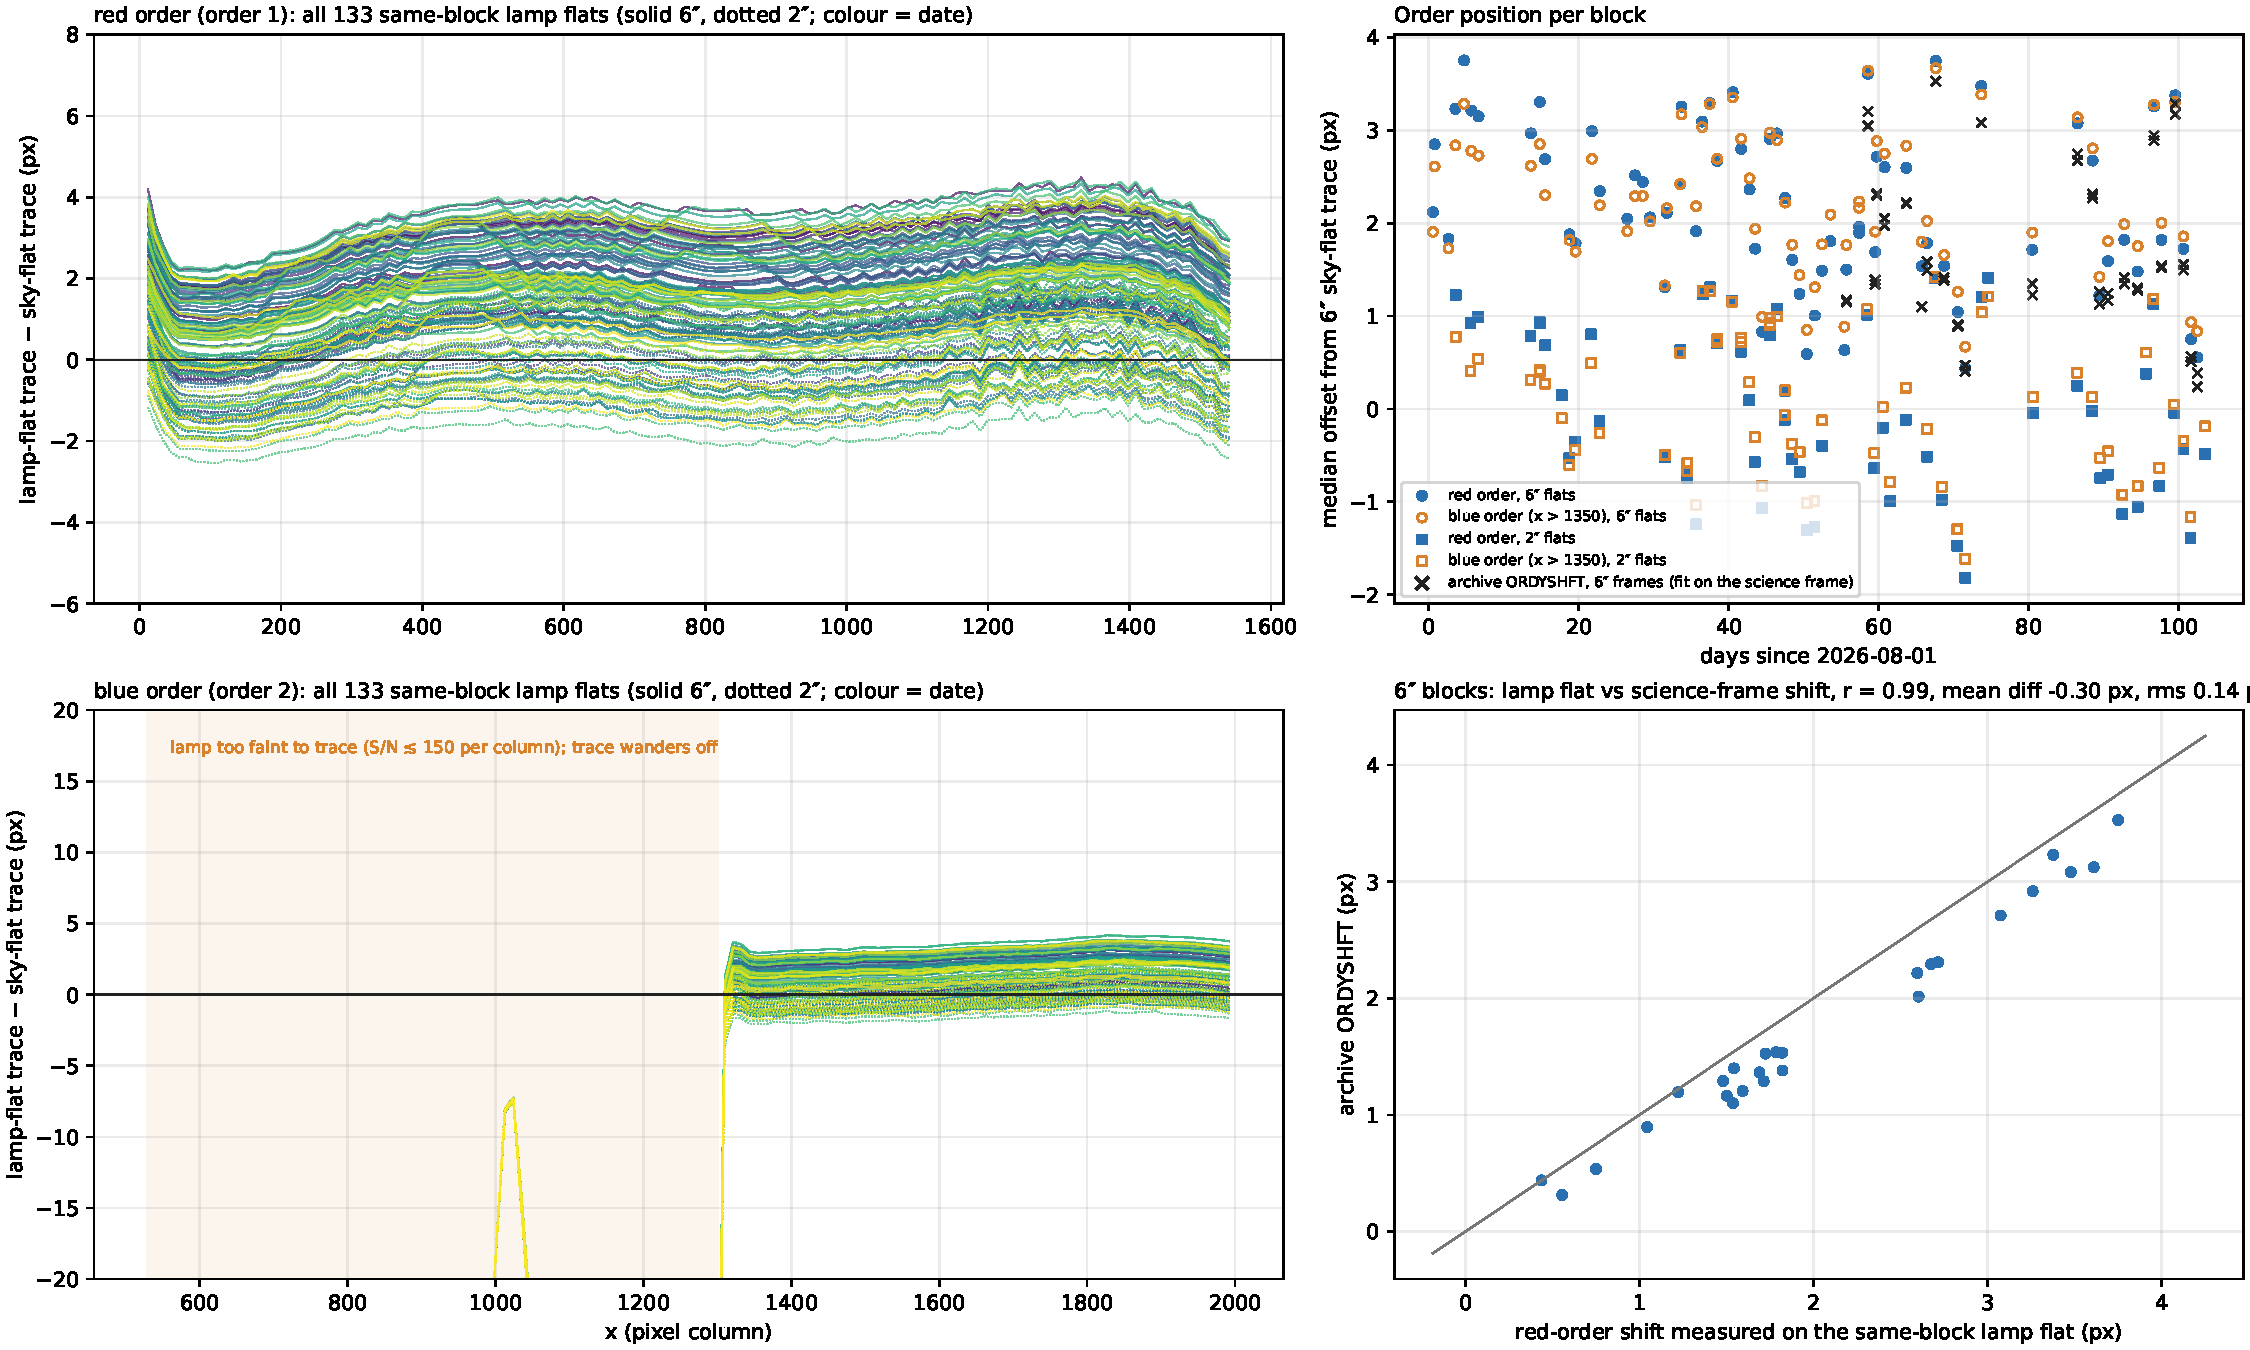
\includegraphics[width=\textwidth]{figures/fig_order_lampflat.pdf}
\caption{Position of the red order relative to the sky-flat trace. Left: shift measured on each of the 133 raw
lamp flats (filled: 6\,arcsec slit, open: 2\,arcsec) and the archive \texttt{ORDYSHFT} of the 6\,arcsec science
frames (crosses), against date. Right: for the 6\,arcsec blocks, the lamp-flat shift against \texttt{ORDYSHFT} of
the same block.}
\label{fig:order_lampflat}
\end{figure}

\section{How \banzai{} traces the object}
\label{sec:traces_object}
\banzai{} first finds the object in the spatial profile summed over all wavelengths. It then follows the object along
the dispersion in short wavelength intervals (\emph{chunks}): in each chunk the spatial profile is summed and the
centroid of its peak measured, and a polynomial in wavelength is fitted through the chunk centroids.
\banzai{}~1.0.1 used a single degree-7 polynomial over the whole order. \banzai{}~1.1.0 uses degree 5 with a penalty
on the second derivative, a minimum signal-to-noise ratio for each chunk and a limit on the jump between chunks.

\textit{Measurement.} We measured the object centroid independently on all 68 archive frames (50 of Fairall~9, 18
of EG\,21). In chunks of 100\,\AA{} (red order) and 50\,\AA{} (blue order), we collapsed the pixels of the
\texttt{BINNED2D} pixel table of the 2-d product (Section~\ref{sec:data}) onto $y_{\rm order}$ and fitted a Gaussian
plus a linear sky. Two problems of the archive data had to be handled. First, the \banzai{}~1.0.1 background is badly
wrong in the red order at 5200--5800\,\AA{} (it swings between $-360$ and $+950$\,counts), so we fitted our own sky.
Second, in some frames \banzai{}~1.0.1 divided the data by the invalid edge of a shifted lamp flat
(Chapter~\ref{sec:fringe}), which destroyed those pixels. They are not masked, but carry data $\approx0$ with an
uncertainty of $\approx10^{-4}$, so they dominate any inverse-variance weighting. We therefore dropped pixels whose
uncertainty is below 10 per cent of the median in the chunk. Neither the re-extraction of the archive products
(improved v1, Appendix~\ref{sec:app_v1}) nor the reduction from raw has such pixels.

Fig.~\ref{fig:trace_frame} shows a typical frame: the trace follows the object at both ends and in the middle of both
orders. The bright-moon frame of Fig.~\ref{fig:trace_frame_moon} shows the striped region destroyed by the flat
division at $x\approx210$--420 in the red order. On this pair of exposures our centroids appear offset from the trace
by 3\,px at 5350--5850\,\AA{}, which appears as the off-scale 6.7 per cent ``loss'' of the worst Fairall~9 frame in
Fig.~\ref{fig:trace_overview}. This offset is caused by the destroyed pixels, not by an error of the trace.

\begin{figure}[!htbp]
\centering
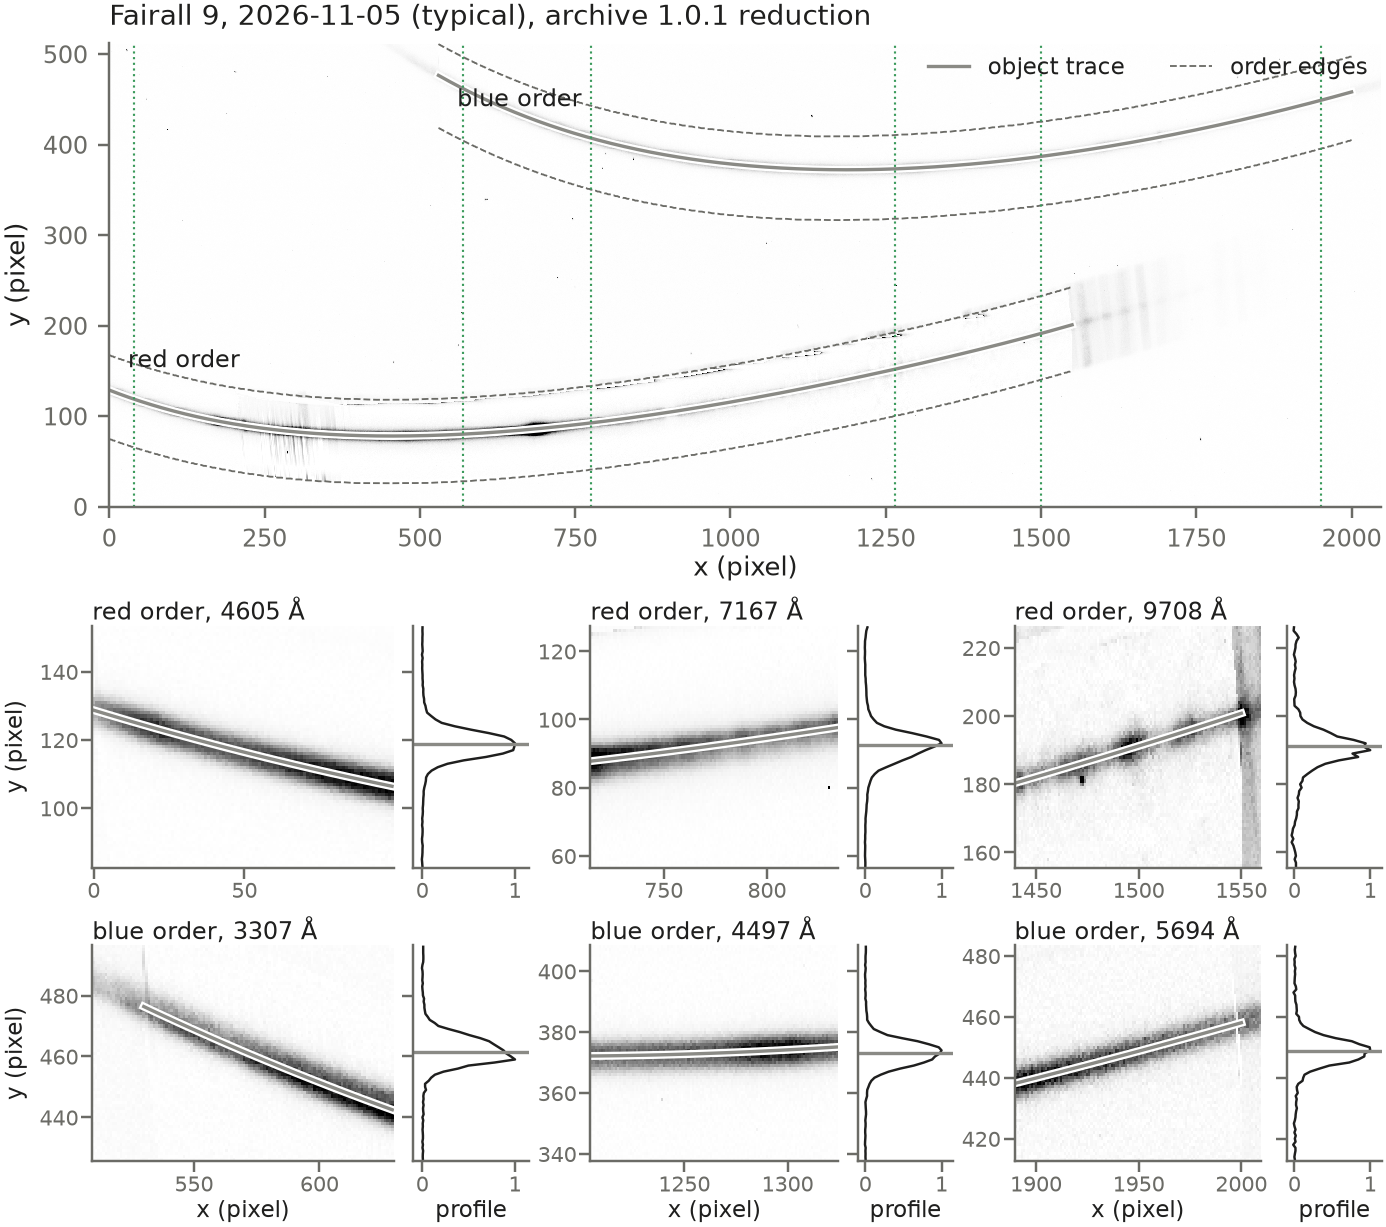
\includegraphics[width=\textwidth]{figures/fig_trace_frame_typical.png}
\caption{Fairall~9, 2026-11-05: background-subtracted archive frame with the order edges (dashed) and the
\banzai{}~1.0.1 object trace (grey with a white outline). The six zooms (green dotted lines) are at the two ends and
the middle of each order; next to each, the spatial profile (median over $\pm12$ columns) with the trace position.}
\label{fig:trace_frame}
\end{figure}

\begin{figure}[!htbp]
\centering
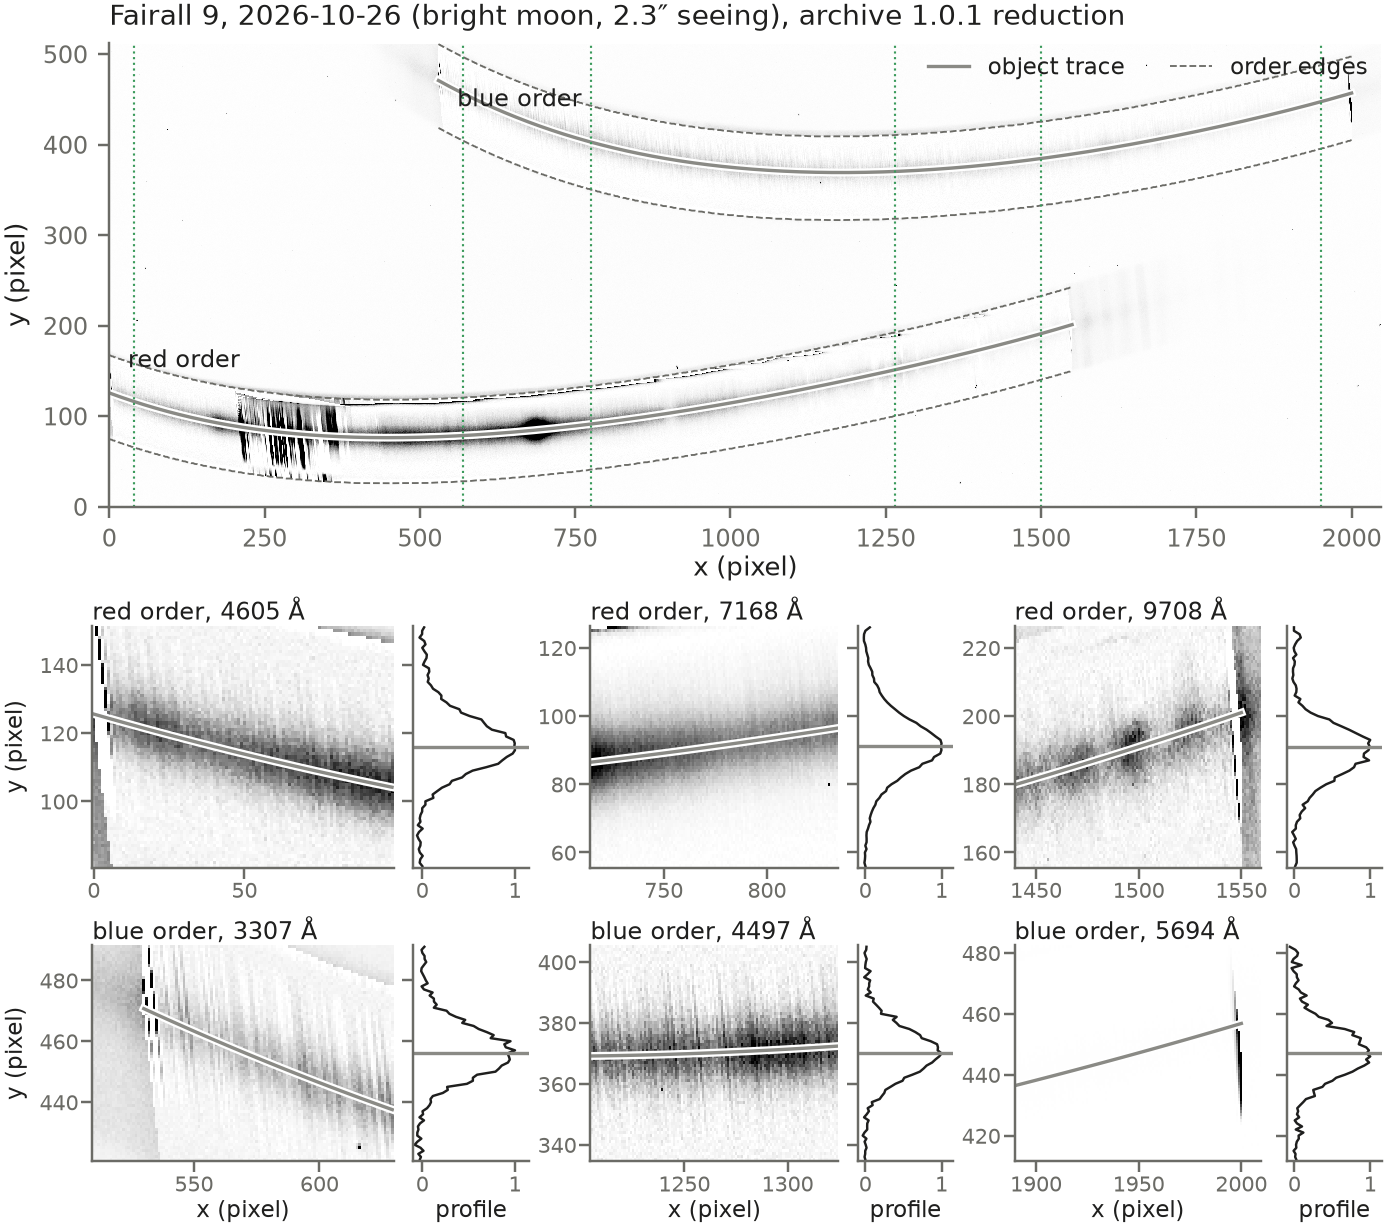
\includegraphics[width=\textwidth]{figures/fig_trace_frame_moon.png}
\caption{As Fig.~\ref{fig:trace_frame} for the bright-moon frame 2026-10-26 \#13 (2.3\,arcsec seeing). The striped
block at $x\approx210$--420 in the red order is where \banzai{}~1.0.1 divided by the invalid edge of the shifted
lamp flat.}
\label{fig:trace_frame_moon}
\end{figure}

\textit{Result.} The median offset between the measured centroid and the archive trace is 0.03\,px, and the flux loss
(eq.~\ref{eq:tracebias}) is below 0.1 per cent at nearly every wavelength (Fig.~\ref{fig:trace_overview}). The
exception is the faint red end, 9250--9750\,\AA. There the offsets reach 0.8--1.4\,px and the loss 1--2 per cent on
the worst frames, because the signal-to-noise ratio per chunk falls to 60--170 and the degree-7 polynomial is barely
constrained. These large offsets are much larger than the noise of the centroids (Fig.~\ref{fig:trace_snr}): they
come from the polynomial, which is poorly constrained at the ends of the fitted range.

\begin{figure}[!htbp]
\centering
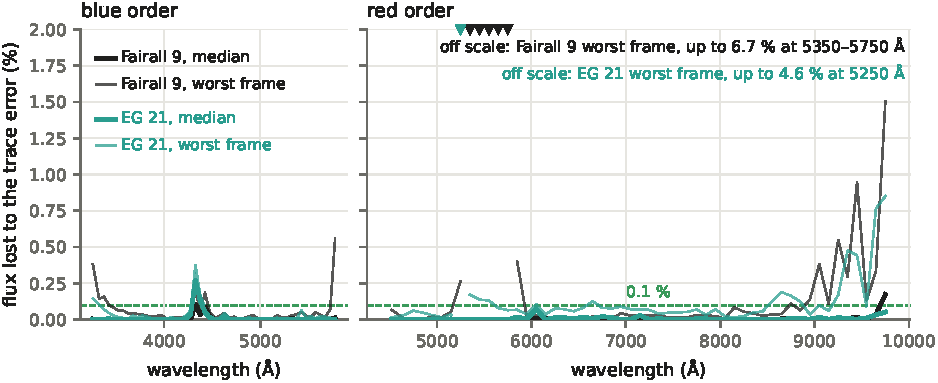
\includegraphics[width=\textwidth]{figures/fig_trace_overview.pdf}
\caption{Flux lost by the optimal extraction because of the error of the archive (1.0.1) object trace
(eq.~\ref{eq:tracebias}), per chunk: median (thick) and worst frame (thin) of the Fairall~9 and EG\,21 archive
frames. Dashed line: 0.1 per cent. Values above the axis are marked at the top edge with their peak value.}
\label{fig:trace_overview}
\end{figure}

\begin{figure}[!htbp]
\centering
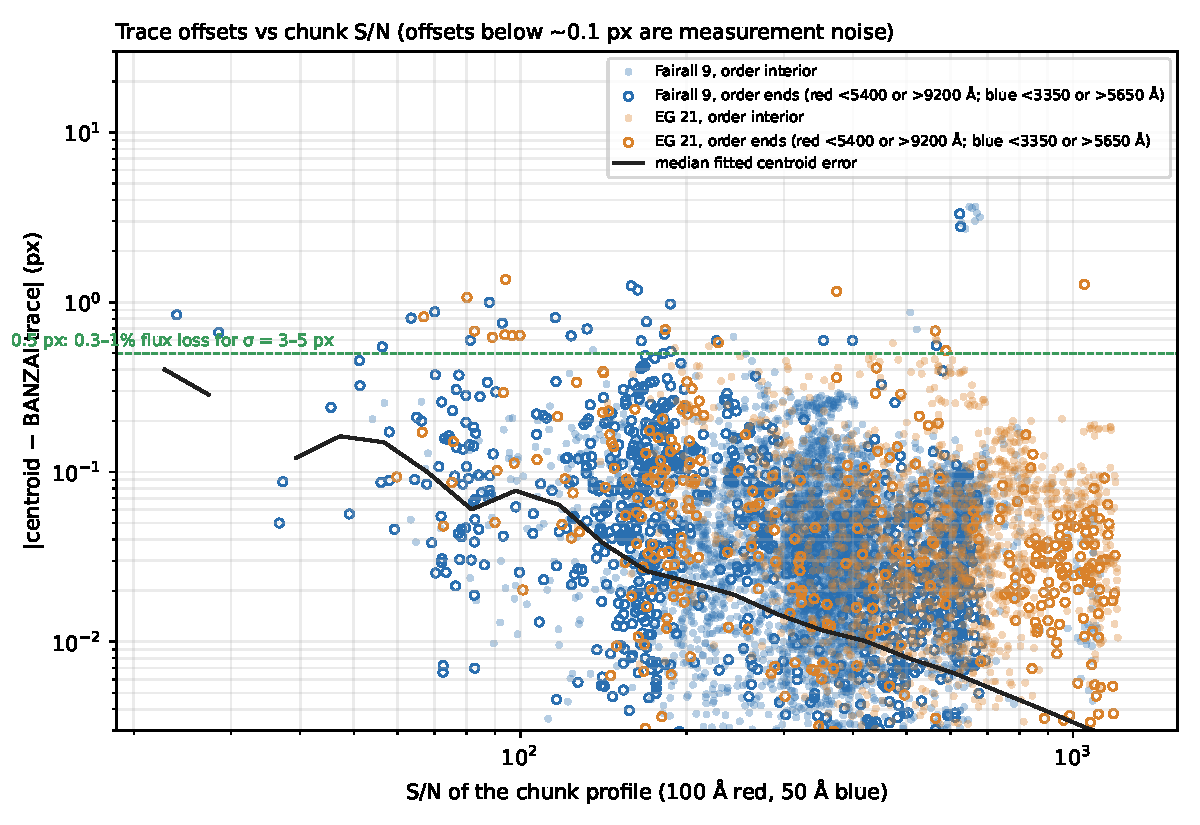
\includegraphics[width=0.75\textwidth]{figures/fig_trace_snr.pdf}
\caption{Absolute trace offset against the signal-to-noise ratio of the chunk; open symbols are chunks at the order
ends. Offsets below $\approx0.1$\,px are measurement noise (black line: median fitted centroid error).}
\label{fig:trace_snr}
\end{figure}

\section{A physical model of the object trace}
\label{sec:traces_model}
FLOYDS observes with the slit along the parallactic angle (rotator mode `vertical float', header keyword
\texttt{ROTMODE = VFLOAT}). Atmospheric differential refraction therefore moves the object \emph{along} the slit, by
\begin{equation}
\Delta y_{\rm ADR}(\lambda)=\frac{206\,265''}{0.337''}\,\left[n(\lambda)-n(\lambda_0)\right]\tan z ,
\label{eq:adr}
\end{equation}
with $n(\lambda)$ the refractive index of moist air at the measured pressure, temperature and humidity
\citep[the formulae collected by][]{Filippenko1982}, $\lambda_0$ a reference wavelength, $z$ the zenith distance, and
0.337\,arcsec the size of a pixel along the slit. For these frames the difference in position between 3300 and
9800\,\AA{} is 3.8--11.3\,px (median 5.9\,px). We model the object trace as
\begin{equation}
c(\lambda)=c_o+a\,\Delta y_{\rm ADR}(\lambda)+S_o(\lambda),
\label{eq:tracemodel}
\end{equation}
where $c_o$ is the position of the object in order $o$, $a$ scales the refraction, and $S_o(\lambda)$ is a fixed
instrumental shape per order (the part of the trace not described by refraction, e.g. the residual between the
order rectification and the true slit image), measured once on bright standards. Only three numbers are fitted per
frame ($c_1$, $c_2$ and $a$), with Gaussian priors on $c_1-c_2$ and $a$ (values below). We call this the
\emph{physical model}.

In our improved pipeline (improved v2 and v3) the physical model is combined with a correction $R_o(\lambda)$ fitted
to its residuals: a Legendre series of degree 5 with a penalty on its slope, so that it goes flat where nothing is
measured. The result, which we call the \emph{combined model}, is
\begin{equation}
c(\lambda)=c_o+a\,\Delta y_{\rm ADR}(\lambda)+S_o(\lambda)+R_o(\lambda).
\label{eq:tracehybrid}
\end{equation}
Where the chunk centroids are good, $R_o$ follows the structure specific to the frame. Where they are sparse or
noisy, the penalty suppresses $R_o$ and the physical model takes over. The template $S_o$ and the priors
($c_1-c_2=-0.87\pm0.29$\,px, $a=0.58\pm0.14$) were measured on 38 standard-star frames of COJ reduced from raw
(Chapter~\ref{sec:raw}). $S_o$ is tabulated every 50\,\AA{} (red order) and 25\,\AA{} (blue order), smoothed over 5
points, and agrees with the median of the stacked standard-star traces to 0.01--0.02\,px. Its peak-to-peak amplitude
is $\approx1$\,px in both orders. The fitted $a$ is 0.4--0.7 rather than 1. We attribute this to the slit not being
exactly at the parallactic angle and to the order rectification absorbing part of the refraction. Since $a$ is
fitted, only the shape of $\Delta y_{\rm ADR}(\lambda)$ matters. The template and priors are specific to each
instrument: OGG has its own, built in the same way from 100 standard-star frames (Section~\ref{sec:sites_trace}).

\textit{Fainter targets.} To test the regime that matters for faint AGN, we simulated fainter versions of Fairall~9.
We took the chunk centroids that \banzai{}~1.1.0 measured on the 100 Fairall~9 exposures reduced from raw, and made
the target 3--100 times fainter: the centroid error of each chunk was scaled up, noise of that size added, and chunks
below the pipeline's detection threshold dropped. We then refitted the trace with the pipeline's own fitting
functions and compared it with the trace fitted to the original centroids, which we take as the truth
(Table~\ref{tab:tracefaint}). The 1.1.0 polynomial is good up to $\approx10$ times fainter than Fairall~9. At 30 times
fainter its error at the order ends grows to 0.8\,px (90th percentile), and at 60 times to 3.5\,px. The physical
model keeps the error at the ends to 0.3--0.4\,px down to 60 times fainter. The combined model
(eq.~\ref{eq:tracehybrid}) is the best or equal best at every level up to 30 times fainter, including the original
brightness (median error 0.06\,px at the ends, like the polynomial, and 0.03\,px in the interior). At 100 times
fainter most chunks fall below the detection threshold, and a fifth of the frames cannot be traced by any method.

\begin{table}[!htbp]
\centering
\caption{Error of the object trace for simulated fainter versions of the 100 Fairall~9 exposures, with the
pipeline's own fitting functions: median / 90th percentile of $|c_{\rm fit}-c_{\rm true}|$ in pixels in the
interior and at the ends of the orders (red $>9200$\,\AA; blue $<3400$ or $>5650$\,\AA). Frames that could not be
traced at all are not included (in brackets: their number).}
\label{tab:tracefaint}
\begin{tabular}{lcccccc}
\toprule
 & \multicolumn{2}{c}{Polynomial (1.1.0)} & \multicolumn{2}{c}{Physical (eq.~\ref{eq:tracemodel})} &
 \multicolumn{2}{c}{Combined (eq.~\ref{eq:tracehybrid})} \\
Fainter by & interior & ends & interior & ends & interior & ends \\
(factor) & (px) & (px) & (px) & (px) & (px) & (px) \\
\midrule
1 & 0.05 / 0.11 & 0.06 / 0.16 & 0.06 / 0.16 & 0.11 / 0.28 & 0.03 / 0.08 & 0.06 / 0.16 \\
10 & 0.05 / 0.12 & 0.10 / 0.27 & 0.06 / 0.17 & 0.12 / 0.30 & 0.03 / 0.09 & 0.08 / 0.21 \\
30 & 0.06 / 0.19 & 0.18 / 0.79 (1) & 0.07 / 0.21 & 0.13 / 0.32 & 0.05 / 0.16 & 0.12 / 0.34 \\
60 & 0.11 / 0.43 & 0.75 / 3.51 (6) & 0.09 / 0.28 & 0.15 / 0.38 (5) & 0.08 / 0.31 & 0.17 / 0.55 (5) \\
100 & 0.20 / 0.71 & 0.66 / 1.84 (19) & 0.17 / 0.58 & 0.24 / 0.65 (16) & 0.17 / 0.62 & 0.26 / 0.87 (16) \\
\bottomrule
\end{tabular}
\end{table}

\textit{On the real data.} The combined model is the default of improved v3 (pipeline setting
\texttt{PROFILE\_TRACE\_MODEL = 'adr'}). On the 157 frames reduced from raw (100 Fairall~9, 18 EG\,21, 39 Feige\,110),
its traces are slightly better than those of \banzai{}~1.1.0 (stock) in every measure (Table~\ref{tab:tracereal}).
The flux loss at the order ends (90th percentile) drops from 0.15--0.19 to 0.11--0.13 per cent. For bright targets
the trace was never a problem; the change matters for faint ones.
Fig.~\ref{fig:trace_compare} compares the archive and the improved v3 traces with the measured centroids on three
frames. On the typical frame the archive trace follows the centroids more closely than the improved v3 trace (rms 0.09
against 0.21\,px); the improved v3 trace departs by up to 0.7\,px at the blue end of the blue order. On the frame with a
faint red end, and on EG\,21, it is the other way round. There the archive polynomial bends away beyond 9600\,\AA{}
(by up to 0.9 and 1.4\,px respectively), while the improved v3 trace stays within 0.8\,px everywhere. The rms of the
archive and improved v3 traces are 0.20 and 0.17\,px on the faint-red-end frame, and 0.36 and 0.24\,px on EG\,21.

\begin{table}[!htbp]
\centering
\caption{Trace offsets on the frames reduced from raw: measured centroid minus trace, median / 90th percentile
(pixels), and the 90th percentile of the flux loss at the order ends.}
\label{tab:tracereal}
\begin{tabular}{llccc}
\toprule
Frames & Trace & interior & ends & loss at ends \\
 & & (px) & (px) & (\%) \\
\midrule
Fairall~9 (100) & 1.1.0 polynomial & 0.075 / 0.22 & 0.10 / 0.37 & 0.15 \\
 & combined model & 0.064 / 0.21 & 0.09 / 0.30 & 0.11 \\
EG\,21 (18) & 1.1.0 polynomial & 0.074 / 0.23 & 0.10 / 0.43 & 0.19 \\
 & combined model & 0.060 / 0.22 & 0.08 / 0.33 & 0.11 \\
Feige\,110 (39) & 1.1.0 polynomial & 0.077 / 0.25 & 0.10 / 0.42 & 0.19 \\
 & combined model & 0.063 / 0.25 & 0.08 / 0.35 & 0.13 \\
\bottomrule
\end{tabular}
\end{table}

\begin{figure}[!htbp]
\centering
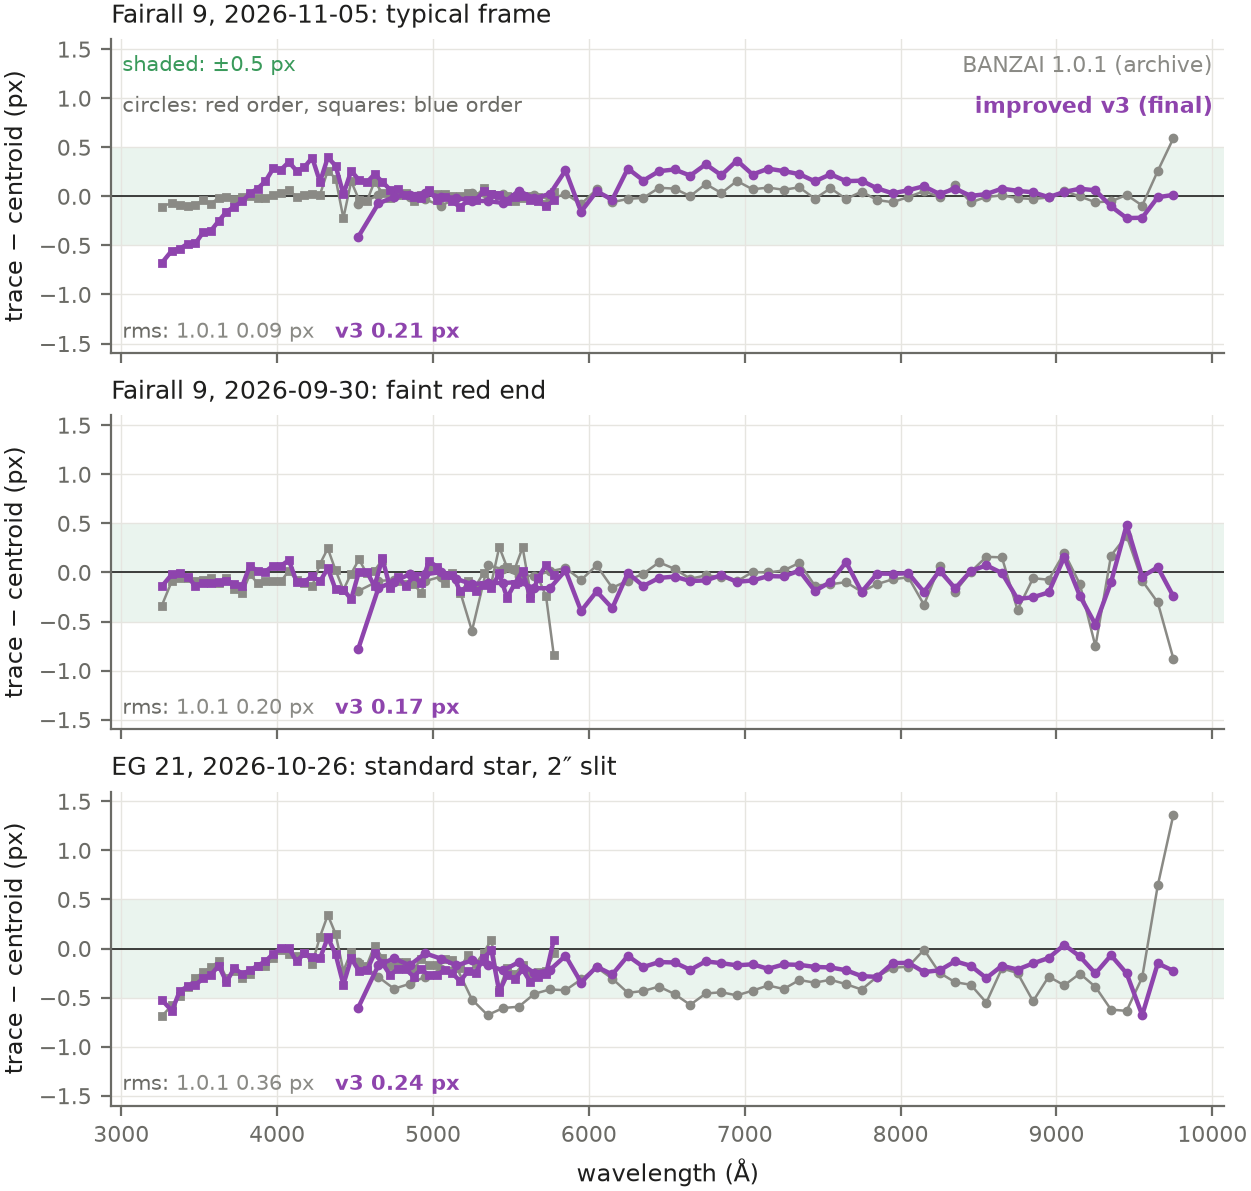
\includegraphics[width=\textwidth]{figures/fig_trace_compare_a.png}
\caption{Object trace minus measured centroid against wavelength for three frames: the archive \banzai{}~1.0.1
trace (grey) and the improved v3 trace (purple, combined model); circles red order, squares blue order; shaded
$\pm0.5$\,px. The archive trace is compared with centroids measured on the archive frame, the improved trace with
centroids measured on the same exposure reduced from raw. The rms over both orders is given in each panel. The
Gaussian centroids are offset by $\approx0.2$\,px from the matched-filter traces in parts of the red order because the
profile is not exactly Gaussian; only the variation with wavelength matters.}
\label{fig:trace_compare}
\end{figure}

\chapter{Wavelength calibration}
\label{sec:wavelength}

This chapter uses the orders, slits, arcs and reduction names defined in the Conventions, p.~\pageref{sec:conventions}. It shows
that the archive wavelength scale has two separate problems: the arc solution has no lines near H$\beta$ and
H$\alpha$, and the wavelength zero point of a compact object in the 6\,arcsec slit changes with its position in the
slit. We correct both.

\section{How \banzai{} calibrates wavelengths}
\label{sec:wl_banzai}
\banzai{} derives the wavelength solution from the arc of each block in five steps. (1) It collapses each order along
the slit, following an assumed line tilt, and finds and identifies the emission peaks. (2) It measures the centroid of each
bright, isolated line in every row with a Gauss--Hermite profile \citep{Cappellari2017}, and fits blended lines with a
fixed line-spread function. (3) For each line it fits a straight line $x=a+b\,y_{\rm o}$, where $x$ is the column,
$y_{\rm o}$ the row relative to the order centre, and the slope $b$ gives the tilt of the line. (4) It fits the column
$x(\lambda)$ of the lines as a Legendre series in wavelength, of degree 5 in the red order and 2 in the blue in
\banzai{}~1.1.0 (the 1.0.1 archive products use degrees 4 and 2). (5) It inverts this to obtain $\lambda(x)$. At COJ
the tilt is a constant ($\approx8.2^\circ$). The final fit has no outlier rejection. There is also no per-exposure
correction of the zero point for flexure or for the position of the object in the slit: every science frame inherits
the solution of its arc.

\section{The arc line list leaves the H$\beta$ and H$\alpha$ regions unconstrained}
\label{sec:wl_lines}
Of the 68 lines in the \banzai{} arc-line catalogue, 33 are used in the fit. In the blue order the solution rests on
Hg lines only: 3650/3663 (a blend), 4047, 4078 and 4358\,\AA, and then 5461, 5770 and 5791\,\AA{}. There is no line
between 4358 and 5461\,\AA{}, exactly where H$\beta$ and [O\,{\sc iii}] fall for $z\lesssim0.1$. The red order
starts at $\approx4550$\,\AA{}, but its first used line is at 5461\,\AA{}, so the solution at 4550--5461\,\AA{} is
an extrapolation. The red order also has no line between 5791 and 6965\,\AA{}, where H$\alpha$ falls for
$z\approx0.05$. The Zn lines that would fill the blue gap are disabled in the \banzai{} line list, with the comment
``removed until we start turning on the Zn lamp again''.

To see which other lines are present, we collapsed all 64 raw arcs (Table~\ref{tab:data}) along the slit using the
2-d wavelength map of a science frame, and aligned them by cross-correlation. The night-to-night shifts are
1.07\,\AA{} rms in the red order and 0.49\,\AA{} in the blue. Three facts follow (Fig.~\ref{fig:arcs}):
\begin{enumerate}
\item[(i)] Hg\,4916 is detected in every single 60\,s arc in both orders, and Ar\,6416, 6677 and 6753/6767 in the red
order, so no stacking is needed to use them.
\item[(ii)] Although the Zn lamp is ``on'' in 63 of the 64 headers, no Zn line is detected, even in the stack of all
64 arcs.
\item[(iii)] Through the 6\,arcsec slit every line is a top-hat (the image of the slit) $\approx51$\,\AA{} wide in the
red order and $\approx25$\,\AA{} in the blue, so many neighbouring lines blend.
\end{enumerate}

\begin{figure}[!htbp]
\centering
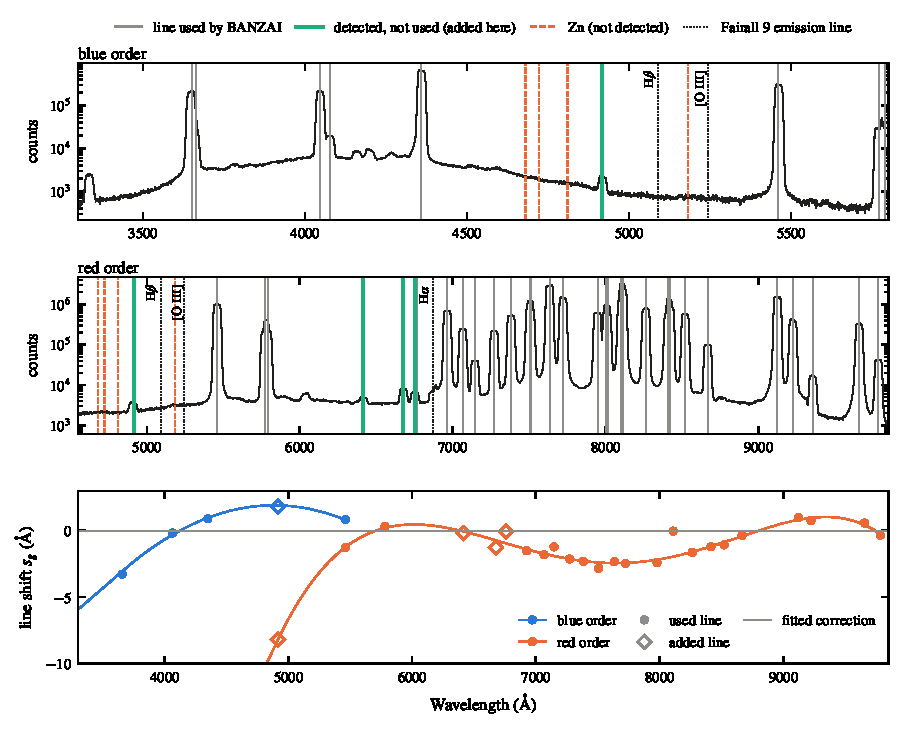
\includegraphics[width=\textwidth]{figures/fig_arcs.pdf}
\caption{Arc lines. Top and middle: one 60\,s arc (6\,arcsec slit) in the blue and red orders. Grey: lines used by
\banzai; aqua: lines detected but not used (Hg\,4916, Ar\,6416, 6677, 6753); dashed orange: Zn lines (lamp ``on''
in the headers, not detected); dotted: H$\beta$, [O\,{\sc iii}] and H$\alpha$ of Fairall~9. Bottom: shift $s_g$ of each
line group (eq.~\ref{eq:arcgroup}) on the \banzai{} solution of 2026-10-08 (circles: used lines; open diamonds: added
lines) and the fitted correction (eq.~\ref{eq:arccorr}). The red order's extrapolated end is off by $-8$\,\AA{} at
Hg\,4916.}
\label{fig:arcs}
\end{figure}


\section{Arc refit with the unused lines}
\label{sec:wl_refit}
For the archive products (improved v1) we measured the error of the archive solution at all detected lines and
corrected it afterwards. Each raw arc is overscan-subtracted and trimmed. It is then collapsed with the frame's own
2-d wavelength map, which already contains the line tilt: all pixels within 30 rows of the order centre are averaged
in wavelength bins of half a pixel. Lines that blend are measured together, in \emph{groups} $g$ with laboratory
wavelengths $\lambda_{g,j}$ (Table~\ref{tab:groups}), with the model
\begin{equation}
M_g(\lambda) = c_0 + c_1\frac{\lambda-\bar\lambda_g}{100} + \sum_j A_j\,B(\lambda;\lambda_{g,j}+s_g,W,\sigma),
\label{eq:arcgroup}
\end{equation}
\begin{equation}
B(\lambda;\mu,W,\sigma)=\frac{1}{2}\left[\mathrm{erf}\!\left(\frac{\lambda-\mu+W/2}{\sqrt2\,\sigma}\right)
 -\mathrm{erf}\!\left(\frac{\lambda-\mu-W/2}{\sqrt2\,\sigma}\right)\right].
\label{eq:boxcar}
\end{equation}
Here $c_0+c_1(\lambda-\bar\lambda_g)/100$ is a linear background, with $\bar\lambda_g$ the mean wavelength of the
group, and $B$ is a top-hat of the width $W$ of the slit image convolved with a Gaussian of width $\sigma$. There is
one such profile per line, at the laboratory separations, with free amplitudes $A_j\ge0$ and a common shift $s_g$:
the measured minus the laboratory wavelength on the solution being tested. The initial width is
$W=8.5$\,\AA\,arcsec$^{-1}$ (red) or 4.25\,\AA\,arcsec$^{-1}$ (blue) times the slit width. Two lines closer than
$0.3W$ cannot be separated, because their amplitude ratio is degenerate with $s_g$. If both catalogue strengths are
known, they are merged into one line at their strength-weighted mean wavelength; if a strength is unknown, both are
kept with free amplitudes. A group is accepted if the fit converged, $|s_g|<14.5$\,\AA{} and its peak exceeds 10
times the residual noise.

The correction is a weighted Legendre series fitted to the group shifts,
\begin{equation}
\Delta\lambda(\lambda)=\sum_{k=0}^{K}d_k\,L_k(\tilde\lambda),\qquad
w_g = \left(\sigma_{s_g}^2+0.3^2+\delta_g^2\right)^{-1},
\label{eq:arccorr}
\end{equation}
where $L_k$ are the Legendre polynomials with coefficients $d_k$, $K=5$ (red) and 2 (blue), $\tilde\lambda$ is the
wavelength mapped to $[-1,1]$, and $w_g$ is the weight of group $g$. In the weight, $\sigma_{s_g}$ is the statistical
error of $s_g$ from the fit, 0.3\,\AA{} is an error floor and $\delta_g$ is an extra systematic error for
unresolved blends (0.5--1\,\AA{}, Table~\ref{tab:groups}). Groups deviating by more than $4\sigma$ are rejected
iteratively. Outside the wavelength range of the accepted groups the correction is continued linearly from its end
values and slopes, so that a degree-5 fit never extrapolates wildly. The corrected wavelength is
$\lambda'=\lambda-\Delta\lambda(\lambda)$.

The fit to one night's arc leaves residuals of 0.48\,\AA{} rms in the red order (median over nights; 23 groups) and
0.10\,\AA{} in the blue (4 groups). The archive red-order solution is wrong by $\approx-8$\,\AA{} at Hg\,4916 and
$\approx-3$\,\AA{} at 5240\,\AA{} (Fig.~\ref{fig:arcs}, bottom). The shape of the arc solution is stable: after
removing each night's zero point, the solutions of the 50 frames agree to $<0.4$\,\AA{} over most of each order. We
therefore apply the \emph{median} of the nightly corrections to every frame; using each night's own fit only adds fit
noise (Section~\ref{sec:results_wl}).

This refit was designed for the archive products (improved v1). The arc fit of \banzai{}~1.1.0, run from the raw
frames, is already far better than the 1.0.1 solution: on the same arcs it is off at the unused lines by at most
0.6\,\AA{} instead of $-8$\,\AA. In the final pipeline (improved v3) the unused lines are added to the arc fit itself.
This brings the remaining error at Hg\,4916 to $\approx0.1$\,\AA{} in the red order (Section~\ref{sec:sites_arcs}),
and no refit afterwards is needed.

\section{The zero point of the object's light}
\label{sec:wl_zp}
The arc and the night sky fill the slit; a compact object does not. In a wide slit the wavelength zero point of the
object therefore depends on where it sits across the slit. A displacement $\Delta\theta$ across the slit moves its
spectrum by $\Delta x=\Delta\theta/0.337''$ pixels, i.e. by $\approx10$\,\AA{} per arcsec in the red order. Neither
the arc nor the sky lines can measure this, because both fill the slit. The telluric absorption bands can
(Section~\ref{sec:diag_tell}): they are imprinted on the object's own light, at wavelengths fixed by the atmosphere.
For each band $b$ we measure the shift $s_b$ of the band in the object spectrum relative to a transmission template
(eq.~\ref{eq:tell}). We subtract the band's offset $o_b$ relative to the O$_2$ A band (Table~\ref{tab:bands},
calibrated on the 18 EG\,21 spectra after the arc refit). We then combine the bands into one red-order shift,
\begin{equation}
s_{\rm red}=\frac{\sum_b \omega_b\,(s_b-o_b)/(\sigma_{s_b}^2+0.5^2)}{\sum_b \omega_b/(\sigma_{s_b}^2+0.5^2)},
\label{eq:tellcomb}
\end{equation}
where $\sigma_{s_b}$ is the error of $s_b$, 0.5\,\AA{} is an error floor, and $\omega_b$ is a weight per band (1 for
the A band, 0.5 for the B band and the H$_2$O band at 7200\,\AA, 0.25 for the H$_2$O band at 9300\,\AA). Bands
deviating by more than $3\sigma$ are rejected iteratively. Both orders image the same slit, so the blue-order shift in pixels is the red-order one times the ratio $\rho$ of
the anamorphic magnifications of the two orders:
\begin{equation}
s_{\rm blue} = \rho\,\frac{s_{\rm red}}{D_{\rm red}}\,D_{\rm blue},\qquad \rho=1.13,
\label{eq:transfer}
\end{equation}
with $D$ the dispersion of each order (\AA\,pixel$^{-1}$). We measured $\rho$ once, as the slope of the blue-order
[O\,{\sc iii}] pixel shift against the red-order A-band pixel shift in the Fairall~9 frames (slope 1.13--1.14,
$r=0.99$, residual 0.2\,pixel); it is an instrument constant. The corrected wavelengths are
$\lambda''=\lambda'-s_{\rm order}$, with $s_{\rm order}$ equal to $s_{\rm red}$ or $s_{\rm blue}$. If no band is usable,
the zero point from the sky lines (Section~\ref{sec:diag_sky}) is used instead; this corrects flexure but not the
position in the slit.

This method ties the wavelength scale to the telluric template, so its absolute zero point is that of the template.
It is uncertain by $\approx\pm4$\,\AA. On the standards the A band lies $-3.5\pm0.7$\,\AA{} from the sky lines (if
the standards are centred in the slit), whereas the [O\,{\sc iii}] lines of Fairall~9 imply $+3.9$\,\AA{} (if
[O\,{\sc iii}] is at the systemic redshift). This uncertainty is a single constant for all frames. It does not affect
the agreement between exposures or between the two orders.

\section{Results}
\label{sec:results_wl}
Fig.~\ref{fig:zeropoint} shows the wide-slit problem in the archive products. From exposure to exposure, the
blue-order [O\,{\sc iii}] wavelength of Fairall~9 scatters by 2.8\,\AA{} rms, whereas the 5577\,\AA{} sky line on the
same frames scatters by only 0.4\,\AA. The object's shift in pixels correlates with the shift of the telluric A band
measured in the red order ($r=0.99$), and not with that of the sky lines. The [O\,{\sc iii}] wavelengths measured in
the red and blue orders differ by $-5.9\pm3.0$\,\AA.

\begin{figure}[!htbp]
\centering
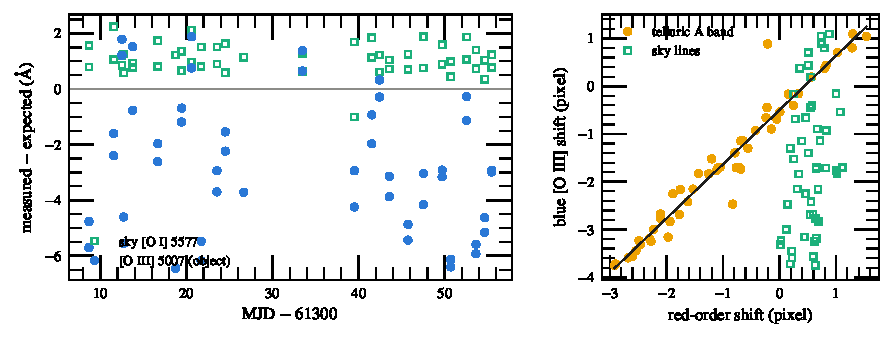
\includegraphics[width=\textwidth]{figures/fig_zeropoint.pdf}
\caption{Left: blue-order [O\,{\sc iii}] shift of Fairall~9 (filled) and 5577\,\AA{} sky-line shift (open) per exposure
in the archive products. Right: blue-order [O\,{\sc iii}] pixel shift against the red-order A-band (filled) and sky-line
(open) pixel shifts; the line has slope 1.13.}
\label{fig:zeropoint}
\end{figure}


After the arc refit and the telluric zero point (Fig.~\ref{fig:redshift}, Table~\ref{tab:summary}) the nuclear
narrow lines agree from exposure to exposure to 20--40\,\kms{} in both orders, and the two orders agree with each
other to $\approx10$\,\kms. Applying each night's own arc fit instead of the median correction increases the scatter
of the red--blue difference from 0.6 to 1.0\,\AA. This confirms that the shape of the arc solution is stable and that
the per-night fit only adds noise.

Two further tests support the method. (i) Before correction, the shifts of [O\,{\sc iii}] and [Ne\,{\sc iii}] follow
the applied zero point with slopes 0.94 and 0.96, whereas the Ca\,{\sc ii}\,K absorption of the host galaxy follows
it with slope 0.17. The host is extended and fills the slit, like the sky. The correction is therefore right for the
nuclear light that RM measures, but not for the host starlight, which matters for decompositions of the host
spectrum. (ii) In the corrected spectra, the cleaner red order yields [O\,{\sc i}]\,6300 in \OIN{} of the 50 spectra, at
\OIvel\,\kms, while [O\,{\sc iii}] sits at \OIIIvel\,\kms. [O\,{\sc iii}] is thus $\approx150$\,\kms{} bluer than
[O\,{\sc i}], a typical signature of an [O\,{\sc iii}] outflow; this bounds the absolute zero-point error at
$\approx2$\,\AA.

\begin{figure}[!htbp]
\centering
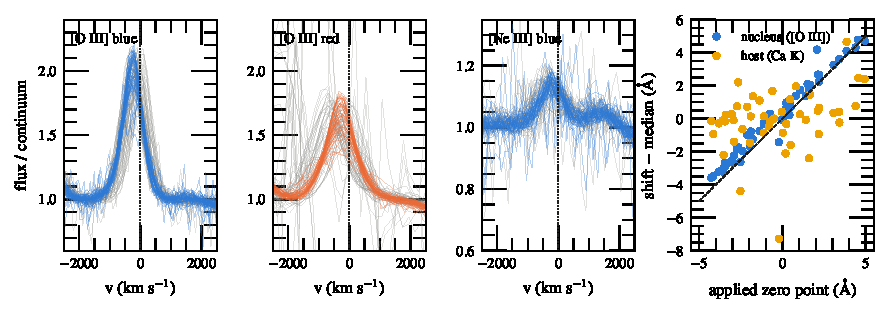
\includegraphics[width=\textwidth]{figures/fig_redshift.pdf}
\caption{Narrow lines of the 50 Fairall~9 spectra in velocity relative to $z=0.047016$: archive (grey) and this work
(colour). Right: shift in the archive products against the applied blue-order zero point for [O\,{\sc iii}] (nucleus)
and Ca\,{\sc ii}\,K (host); dashed: slope 1.}
\label{fig:redshift}
\end{figure}



\chapter{Fringing}
\label{sec:fringe}

\textit{The problem.} Beyond $\approx6500$\,\AA{} the FLOYDS red order shows fringes: an interference pattern of the
CCD that modulates the spectrum by up to 10--20 per cent with a period of $\approx38$\,\AA{}
(see the Conventions, p.~\pageref{sec:conventions}). Because reverberation mapping compares spectra taken on different nights, the
fringes must be removed from every single spectrum, not only on average.

\textit{What the archive does.} \banzai{}~1.0.1 divides each 2-d frame by a whole lamp flat taken months earlier,
shifted along the slit by a fitted offset. This removes the fringes poorly, imprints the lamp's own illumination
pattern on the science, and in some frames destroys pixels (Section~\ref{sec:fringe_banzai}).

\textit{What we changed.} The frame is no longer divided by a flat. Instead, the fringes are fitted in each extracted
1-d spectrum with a \emph{harmonic model}: a sum of sine waves whose phase is taken from the lamp flats and whose
amplitude and shape are fitted to the spectrum itself (Section~\ref{sec:fringe_harmonic}). Inside the pipeline the
model was then refined in the 6500--7500\,\AA{} region and fitted jointly with the telluric absorption
(Sections~\ref{sec:fringe_pipeline} and \ref{sec:fringe_joint}).

\textit{How much better.} The fringe metric of Table~\ref{tab:summary} (the rms of the ratio of 25 and 200\,\AA{}
running medians in the telluric-free windows 7750--8050 and 8450--8900\,\AA) of the Fairall~9 spectra drops from 13.7
per cent in the archive and 8.1 per cent in \banzai{}~1.1.0 to 1.9 per cent in improved v3
(Table~\ref{tab:versions}). In this chapter, names in typewriter font are the corresponding \banzai{} settings,
header keywords or scripts, given for readers who want to reproduce the results.

\section{What \banzai{}~1.0.1 does}
\label{sec:fringe_banzai}
Each archive \texttt{-2d} product stores, in its \texttt{FRINGE} extension, the map $\Phi(x,y)$ by which
\banzai{}~1.0.1 divided the frame. Inspecting these maps, we find four problems:
\begin{enumerate}
\item $\Phi$ is a whole normalised lamp flat (taken 2026 March 14/15, eight months before the science), not only its
fringe component. Besides the fringes it contains the lamp's illumination profile along the slit (bands of
$\pm5$ per cent at 5000--7000\,\AA) and flat-field structure. It is applied from $\approx5000$\,\AA{}
(Fig.~\ref{fig:master}).
\item The map is shifted \emph{along the slit} by an offset fitted to each frame (header keyword
\texttt{L1FRNGOF}). Cross-correlating the maps of two frames gives a shift equal to the difference of their offsets
(17 rows for offsets $+9.0$ and $-8.5$). The fitted offsets range from $-575$ to $+182$\,pixels and cluster near
$\pm9$ and $\pm14$\,pixels, where the periodic fringe pattern gives false matches; the real flexure is only
1--2\,pixels.
\item Where the shifted map has no data (rows shifted in from beyond the edge of the flat), it holds either
quantisation noise ($\sim10^{-6}$) or values up to $\pm3\times10^4$. In 13 of the 50 Fairall~9 frames (all with
offsets between $-8.5$ and $-11.1$) this invalid edge falls inside the illuminated order at 5200--5700\,\AA{}. The
pixels there are divided by values $\gg1$, the 2-d sky model oscillates into stripes, and the extraction turns these
into 25--127 spikes per spectrum (Fig.~\ref{fig:edge}).
\item Because the whole flat is used, every frame is divided by the lamp's illumination profile at the rows where the
object lies. This is a factor of up to $\pm10$ per cent that depends on the frame and on wavelength (a 15 per cent
excess at 5500--7000\,\AA{} in a bright-moon frame).
\end{enumerate}

\begin{figure}[!htbp]
\centering
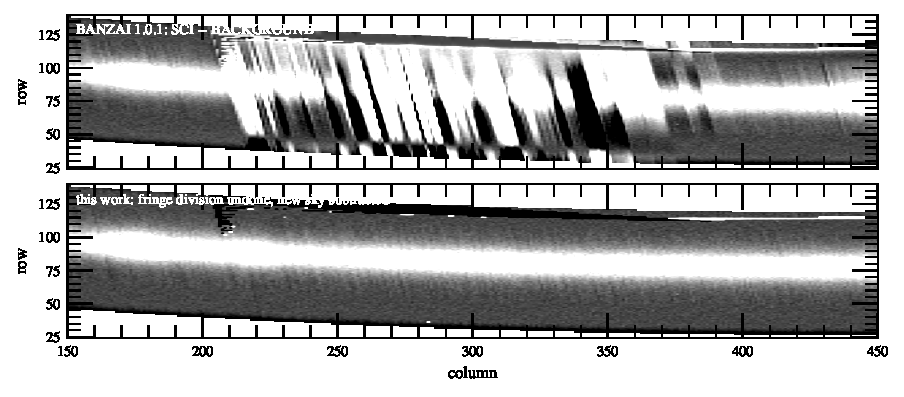
\includegraphics[width=\textwidth]{figures/fig_edge.pdf}
\caption{Red order at $\approx5000$--6000\,\AA{} of the bright-moon frame 2026-10-26 \#13. Top: archive SCI minus
BACKGROUND. Bottom: improved v1 (fringe division undone, invalid pixels masked, new sky subtracted; Appendix~\ref{sec:app_v1}).}
\label{fig:edge}
\end{figure}





\section{Harmonic fringe model}
\label{sec:fringe_harmonic}
\banzai{}~1.1.0, run from the raw frames, no longer divides the frame by the lamp flat. In our reductions from the
raw frames (improved v2 and v3) the fringes are removed from the extracted spectrum with the model of this section. The model was first developed on the archive
products (improved v1), where the 1.0.1 division had to be undone first (Appendix~\ref{sec:app_v1}). In both cases
the input is the fringe component $\delta$ of a lamp-flat pattern: the lamp flat divided by its running median along
the dispersion, which keeps only the fringes. In the pipeline the pattern is the median of the processed lamp flats
of one slit width over one to two months (the phase master, Section~\ref{sec:fringe_pipeline}); for the archive
products it is given by eq.~(\ref{eq:delta}).

\textit{Why a scaled lamp pattern cannot work.} The simplest correction, used in our first version (improved v1),
divides the spectrum by the lamp's fringe pattern multiplied by an amplitude $A(\lambda)$ calibrated per slit width
(the \emph{amplitude law}, Appendix~\ref{sec:app_v1}). Fig.~\ref{fig:harmonic} shows why this is not enough. It
shows the red order of a standard and of a Fairall~9 frame before fringe correction, divided by a smooth continuum.
The fringes have sharp maxima and broad, shallow minima, as expected from the Fabry--P\'erot transmission of the
thinned CCD. The scaled lamp pattern is almost sinusoidal. When its maxima match the data, its minima are too deep
(normalised minima of 0.55--0.6 instead of 0.75--0.8), which produces the asymmetric, spiky residuals of the
amplitude-law correction.

The reason is the range of wavelengths that reaches each pixel. A pixel at column $x$ receives the wavelength
$\lambda_0(x)-D\,s$ from every illuminated position $s$ across the slit, with $D$ the dispersion. The recorded fringe
is therefore the CCD transmission $\mathcal{T}(x,y,\lambda)$ smoothed by the image of the light across the slit, in
wavelength units. For the lamp, which fills the slit, this kernel is a top-hat of the slit width (51\,\AA{} in the red
order for the 6\,arcsec slit, larger than the $\approx38$\,\AA{} fringe period); for a point source it is the seeing
profile. If $\mathcal{T}$ is written locally as a Fourier series in its phase $\phi$, harmonic $k$ is multiplied by
the Fourier transform of the kernel at $k$ times the fringe frequency. A symmetric kernel preserves the phase. The
slit-filling lamp, however, suppresses the fundamental and, much more, the harmonics, by factors that depend on
wavelength (the period grows as $\lambda^2$) and differ from those of the object. The lamp flat therefore gives the
\emph{phase} of the fringes but neither their amplitude nor their shape. In addition, the object's phase is offset
from the lamp's by flexure and by its position across the wide slit, both of which change the wavelength falling on
each pixel: a 5\,\AA{} offset moves the phase by $\approx0.2$ cycles. The free fits below give a frame-to-frame phase scatter of 16--26$^\circ$ for Fairall~9 and
6--9$^\circ$ for EG\,21; a 20$^\circ$ error alone leaves a residual of $2\sin(10^\circ)A\approx0.35A$, about a third of the
fringe amplitude.

\begin{figure}[!htbp]
\centering
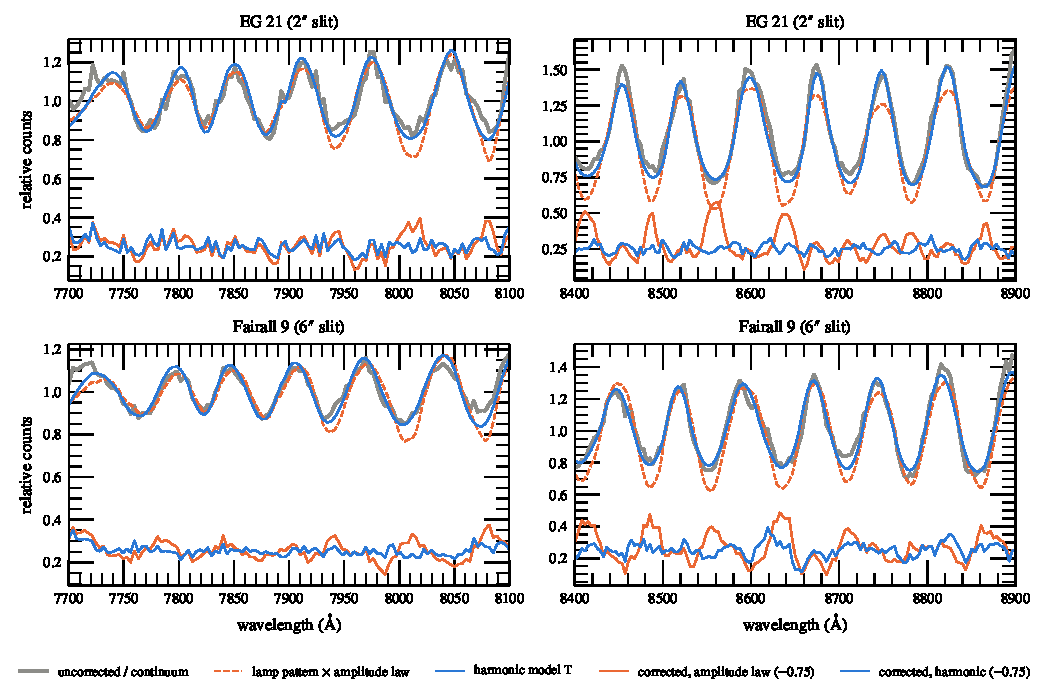
\includegraphics[width=\textwidth]{figures/fig_harmonic.pdf}
\caption{Fringe shape at 8400--8900\,\AA{} in the red order of an EG\,21 frame (left) and a Fairall~9 frame (right).
Top: the extraction before fringe correction over its 150\,\AA{} running median (grey), the lamp pattern times the
amplitude law (dashed; its minima are too deep) and the harmonic model $T$ (eq.~\ref{eq:harmonic}). Bottom: the
spectrum corrected with each model, over its running median; the rms in this window is given above each panel.}
\label{fig:harmonic}
\end{figure}


\textit{Phase map.} For every row of the red order, we take the fringe phase from the lamp-flat fringe component,
smoothed with a Gaussian of $\sigma=1$ pixel, as the argument of its analytic signal:
\begin{equation}
\phi(x,y)=\arg\left\{\tilde\delta(x,y)+i\,\mathcal{Q}_x[\tilde\delta](x,y)\right\},
\label{eq:phase}
\end{equation}
where $\mathcal{Q}_x$ is the Hilbert transform along the dispersion and $\tilde\delta$ the smoothed $\delta$ (eq.~\ref{eq:delta}).

\textit{Model and fit.} The fringe transmission $T(\lambda)$ of the extracted spectrum (the factor by which the
fringes multiply it) is modelled in logarithm as
\begin{equation}
\ln T(\lambda)=\sum_{k=1}^{K}\sum_{j=1}^{J}h_j(\lambda)\left[a_{jk}\,C_{k,\beta}+b_{jk}\,S_{k,\beta}\right],
\label{eq:harmonic}
\end{equation}
\begin{equation}
C_{k,\beta}=\frac{\sum_{i\in\beta}P_iw_i\cos k\phi_i}{\sum_{i\in\beta}P_i},
\label{eq:harmproj}
\end{equation}
Here $\beta$ is a 1-pixel wavelength bin of the extracted spectrum and $i$ runs over the 2-d pixels in that bin, with
phase $\phi_i$ and profile weight $P_i$ (the fraction of the object's light in pixel $i$). $C_{k,\beta}$ is thus the
profile-weighted mean of $\cos k\phi$ in the bin, and $S_{k,\beta}$ is defined likewise with $\sin k\phi_i$. $w_i$ is
the taper of eq.~(\ref{eq:delta}), which switches the model on gradually at the blue end. The $h_j$ are linear
interpolation functions on the nodes $\lambda_j=6800,7300,\dots,9800$\,\AA{} ($J=7$), so the coefficients
$a_{jk},b_{jk}$ are allowed to vary smoothly with wavelength. $k$ is the harmonic number; we use $K=2$
(28 coefficients), and $K=1$ is only slightly worse. The $b_{jk}$ absorb the phase offset of the frame, and the
$a_{jk}$ and $b_{jk}$ together give the amplitude and shape of the fringes. The coefficients are the linear
least-squares solution of
\begin{equation}
\mathcal{H}_{150}[\ln F_\beta]=\sum_{j,k}a_{jk}\,\mathcal{H}_{150}[h_jC_k]_\beta+b_{jk}\,\mathcal{H}_{150}[h_jS_k]_\beta,
\label{eq:harmfit}
\end{equation}
where $F$ is the extraction without fringe correction and $\mathcal{H}_{150}$ subtracts a 150\,\AA{} running median.
The fit uses three iterations of $5\sigma$ clipping. The telluric bands need care. If they are simply excluded,
the coefficients across 8900--9300\,\AA{} are constrained only by the neighbouring regions, and the residual there
is 8--9.5 per cent. The fit is therefore done in two passes. The first excludes
the bands (6860--6960, 7150--7350, 7560--7720, 8100--8380 and 8900--9300\,\AA) and is followed by the wavelength and
flux calibration, which yield the telluric transmission $t$ of each spectrum (Section~\ref{sec:flux_tell}); the second
refits eq.~(\ref{eq:harmfit}) on $F/t$, excluding only the A band and pixels with $t<0.3$. In a test on all frames this
lowers the residual at 8950--9300\,\AA{} from 8--9.5 to 5.3--5.6 per cent and at 9300--9700\,\AA{} from 8.2--8.5 to
6.8--8.5 per cent, with the residual in the clean windows unchanged. The extracted counts and their
uncertainties (both the optimal and the fixed-aperture extraction) are then divided by $T$. The fit uses only the
frame's own spectrum and the phase map, and no information on the target. Because the basis oscillates with the fringe phase, it is nearly orthogonal to
astrophysical structure on scales above $\approx50$\,\AA, and the clipping removes narrow features.

\textit{Variants tested} (Table~\ref{tab:fringevariants}). (i) The phase can be taken from the eight-month-old
master pattern recovered from the archive maps (Appendix~\ref{sec:app_v1}), or from the lamp flat taken in the same
block as each science frame (69 such flats exist for the Fairall~9 campaign, matched by block identifier; command-line
option \texttt{--flat-dir}). Their fringe components correlate with the master at $r=0.95$--0.98, and the harmonic
correction with same-block phases is indistinguishable from the one with the master. The detector pattern is stable
over the eight months, so the age of the flat was not the limiting factor. (ii) The classical approach measures the
fringes on a standard star and transfers them to the science frame. Here we used the high-passed $\ln F$ of the
nearest EG\,21 spectrum, with a free shift and a free scale at each node. It does better than the amplitude law but
worse than the harmonic model, because the phase offset differs between exposures. (iii) For the AGN, fixing the
harmonic coefficients to their median over all frames, or fixing only the amplitude and fitting the phase, is worse
than fitting all coefficients freely in each frame.

\begin{table}
\centering
\caption{Fringe residuals of the red order: rms of $\ln F$ after subtracting a 150\,\AA{} running median, in
7750--8050 and 8450--8900\,\AA, per cent, median over frames. No short smoothing is applied, so photon noise sets a
floor (last row). $^{a}$16 frames with a lamp flat within one day.}
\label{tab:fringevariants}
\begin{tabular}{lcc}
\toprule
Correction & Fairall~9 & EG\,21 \\
 & (\%) & (\%) \\
\midrule
None & \FVnoneF & \FVnoneE \\
Amplitude law (master pattern) & \FVampF & \FVampE \\
Standard-star transfer & \FVstdF & -- \\
Harmonic, ensemble coefficients & \FVensF & \FVensE \\
Harmonic, master phase & \FVharmF & \FVharmE \\
Harmonic, same-block flat phase & \FVflatF & \FVflatE$^{a}$ \\
Photon-noise floor & \FVnoiseF & \FVnoiseE \\
\bottomrule
\end{tabular}
\end{table}

\section{The harmonic model inside the pipeline, and the 6500--7500\,\AA{} region}
\label{sec:fringe_pipeline}
In the reduction from the raw frames (Chapter~\ref{sec:raw}) the frame is never divided by a lamp flat (setting
\texttt{FRINGE\_METHOD = 'harmonic'}). Instead, a new pipeline stage, \texttt{HarmonicFringeCorrector}, fits
eq.~\ref{eq:harmonic} to each extracted spectrum, after the telluric transmission of the standard has been loaded.
The initial configuration used the settings developed on the archive products: phase from the lamp flat of the same
block, model tapered in from 6500\,\AA{} and fully on at 6800\,\AA, amplitude nodes every 500\,\AA{} from
6800\,\AA, and fit on the telluric-corrected spectrum. It matched the archive-based recalibration (improved v1)
redward of 7700\,\AA, but residual fringes were visible at 6500--7500\,\AA{} in the individual Fairall~9 spectra.

We tested twelve variants offline on all 157 frames reduced from the raw data. For each variant, the uncorrected
extraction of each frame was refitted and scored. The stars were scored by the rms of the 12/150\,\AA{} high-pass
(see the Conventions, p.~\pageref{sec:conventions}) in windows free of lines and telluric bands. Fairall~9 has no line-free windows at
these wavelengths, so it was scored by the scatter between its 100 spectra; this measures only the frame-specific
part of the residual, since fringes common to all frames cancel. Table~\ref{tab:fringebench} summarises the result:
\begin{enumerate}
\item Below 6450\,\AA{} the fringes are $\lesssim0.3$ per cent. Starting the model at 5800\,\AA{} only adds noise
(Fairall~9 at 6000--6450\,\AA: 0.93$\rightarrow$1.16 per cent), so the onset stays at 6500\,\AA.
\item The phase of a single 6\,arcsec lamp flat is noisy at 6500--7500\,\AA, where the lamp fringes have little
contrast. The per-frame fit then injects bumps that differ from frame to frame (Fairall~9 at 6450--6850\,\AA:
1.34 per cent, against 0.94 uncorrected). A phase master, the median of the fringe patterns of all lamp flats of one
slit width over one to two months, removes most of this.
\item Fitting on the telluric-corrected spectrum transfers the residuals of the standard's telluric transmission
(Chapter~\ref{sec:flux}) into the fringe model. Masking all telluric bands is better everywhere except redward of
the 8900\,\AA{} water band, where there is no telluric-free stretch left.
\item The phase was taken from the Hilbert transform of the lamp pattern smoothed by one pixel (eq.~\ref{eq:phase}).
But the pattern also contains slow structure: the slit illumination and the shape of the lamp spectrum, 4--5 per cent
rms even at 6000--6500\,\AA{} where there are no fringes. Where the fringe contrast is low, at 6500--7500\,\AA{}
through a wide slit, this slow structure sets the phase, and the fit removes almost nothing: in the individual
Fairall~9 spectra the fringes at 7100--7550\,\AA{} were nearly unchanged by the correction. Removing structure longer
than 31\,px with a running median before the Hilbert transform fixes this. The fringe period grows from
$\approx8$\,px at 7000\,\AA{} to 15--20\,px beyond 8500\,\AA, where a 31\,px filter would affect the fringes
themselves. We therefore use this high-passed phase blueward of 7600\,\AA{} and the plain phase redward of
7900\,\AA, interpolating between the two angles in between (setting \texttt{FRINGE\_PHASE\_HIGHPASS}). On Fairall~9
the rms of the high-passed spectra at 6960--7150\,\AA{} drops from 1.13 to 0.90 per cent (uncorrected 1.37). At
7350--7550\,\AA{} it drops from 3.75 to 3.44 per cent (uncorrected 4.53; He\,{\sc i}\,7065 and
[Ar\,{\sc iii}]\,7136 fall in this window). The stars are unchanged.
\item More harmonics, more phase smoothing or a fixed high-pass at all wavelengths do not help.
\end{enumerate}
The configuration at this stage (improved v2, last row of Table~\ref{tab:fringebench}) used the phase master
(setting \texttt{FRINGE\_PHASE\_SOURCE = 'stacked'}) with the blended high-pass phase, nodes every 400\,\AA{} from
6600\,\AA, and all telluric bands masked. Redward of the 8900\,\AA{} water band, where no band-free stretch is left,
it switches to a fit on the telluric-corrected spectrum, blending the two fits between 8850 and 8950\,\AA{} (setting
\texttt{FRINGE\_TELLURIC\_BLEND}). Both fits are small linear least-squares problems.

\begin{table}[!htbp]
\centering
\small
\caption{Fringe-model variants on the 157 frames reduced from raw. Stars (EG\,21, Feige\,110): median rms (per cent)
of a 12/150\,\AA{} high-pass in line- and telluric-free windows. Fairall~9: small-scale scatter between the
spectra (per cent; frame-specific part only).}
\label{tab:fringebench}
\footnotesize
\setlength{\tabcolsep}{3.2pt}
\begin{tabular}{@{}>{\raggedright\arraybackslash}p{3.7cm}ccccc|ccccc@{}}
\toprule
 & \multicolumn{5}{c|}{Stars: window (\AA)} & \multicolumn{5}{c}{Fairall~9: window (\AA)} \\
 & 6650-- & 6960-- & 7350-- & 7750-- & 8450-- & 6000-- & 6450-- & 6950-- & 7700-- & 8500-- \\
Variant & 6850 & 7150 & 7550 & 8050 & 8900 & 6450 & 6850 & 7550 & 8500 & 9200 \\
 & (\%) & (\%) & (\%) & (\%) & (\%) & (\%) & (\%) & (\%) & (\%) & (\%) \\
\midrule
uncorrected & 1.73 & 3.64 & 5.43 & 11.39 & 26.49 & 0.92 & 0.94 & 1.80 & 3.24 & 4.42 \\
initial configuration & 0.73 & 1.18 & 1.12 & 2.04 & 4.76 & 0.93 & 1.34 & 1.91 & 2.52 & 3.37 \\
onset 5800\,\AA, nodes 400\,\AA & 0.69 & 1.23 & 1.24 & 2.10 & 4.83 & 1.16 & 1.31 & 1.81 & 2.45 & 3.34 \\
\quad + phase master & 0.70 & 1.19 & 1.24 & 2.13 & 4.82 & 1.01 & 1.21 & 1.68 & 2.35 & 3.34 \\
\quad + all bands masked & 0.56 & 1.08 & 1.27 & 1.52 & 3.12 & 1.18 & 1.18 & 1.85 & 2.25 & 4.21 \\
phase master, all bands masked, nodes 400\,\AA{} from 6600 & 0.60 & 1.11 & 0.92 & 1.55 & 2.89 & 0.92 & 1.02 & 1.79 & 2.29 & 3.60 \\
\quad + telluric-corrected fit beyond 8850\,\AA & 0.59 & 1.11 & 0.92 & 1.49 & 2.99 & 0.92 & 1.05 & 1.77 & 2.29 & 3.27 \\
\quad + phase high-pass 31\,px blueward of 7600\,\AA{} (improved v2) & 0.66 & 1.08 & 0.99 & 1.57 & 2.99 & 0.90 & 0.98 & 1.56 & 2.24 & 3.27 \\
\bottomrule
\end{tabular}
\end{table}

\subsection{Joint telluric fit, earlier onset, denser nodes and a residual template}
\label{sec:fringe_joint}
Two problems remained with that configuration.
(i) Inside the water bands (7170--7330 and 8130--8360\,\AA) the Fairall~9 spectra kept 4 per cent rms of structure on
fringe scales (12/150\,\AA{} high-pass), against 1.7--3.2 per cent in the archive-based recalibration (improved v1).
Most of it (3.1 per cent) was common to all spectra. With the bands masked, the fringes inside them are only
interpolated from the band edges. The residual therefore stays in the transmission measured on the standards and,
through the telluric correction with the median of nine standards (Section~\ref{sec:flux_tell}), in every science
spectrum.
(ii) The flux-calibrated standards show wiggles of $\approx1$ per cent redward of 6500\,\AA. Part of this is only a
matter of where the residual becomes visible. The sensitivity function has knots every 20\,\AA{} blueward of
6500\,\AA{} and every 600\,\AA{} redward (Chapter~\ref{sec:flux}), so a residual of the same size is absorbed by the
sensitivity in the blue and remains visible in the red. But the raw counts do have fringes of 1--2 per cent already
at 6300--6500\,\AA{} and $\approx3$ per cent at 6500--6800\,\AA, where the model was only being tapered in.

We tested four changes on all 157 frames. For each, the standards' telluric transmissions, the nine-standard
ensembles and the science spectra were rebuilt offline (Table~\ref{tab:fringejoint}):
\begin{enumerate}
\item \textit{Joint fit.} The fringes are fitted together with the logarithm of a smooth telluric template
(\citealt{Matheson2000}, convolved to 9\,\AA), one free depth per band (6255--6335, 6850--7090, 7135--7400,
7870--8050 and 8085--8400\,\AA, the bands of Section~\ref{sec:flux_tell}). Only the saturated O$_2$ A band and the
8900--9300\,\AA{} water band stay masked (setting \texttt{FRINGE\_JOINT\_TELLURIC}). The fringes inside the bands
are then fitted against the shape of the absorption instead of being interpolated. This helps only when applied to
every frame; applied to the standards alone, it leaves the science spectra unchanged. The fringe metric and the
residual in the clean windows are not affected.
\item \textit{Onset.} The model is switched on gradually from 6200\,\AA, reaching full strength 200\,\AA{} later
(settings \texttt{FRINGE\_HARMONIC\_ONSET} and \texttt{FRINGE\_HARMONIC\_TAPER}). The 6400--7550\,\AA{} residual of
the standards drops from 0.90 to 0.81 per cent; Fairall~9 is unchanged. Starting at 6000\,\AA{} is worse.
\item \textit{Nodes every 200\,\AA.} The amplitude and phase offset of the fringes change along the order faster
than nodes every 400\,\AA{} can follow, and the 6\,arcsec spectra are the most affected. With nodes every 200\,\AA,
the Fairall~9 water-band residuals drop to 1.8 and 3.3 per cent, as good as the archive-based recalibration, and the
fringe metric drops to 2.0 per cent. The 2\,arcsec stars become slightly noisier (EG\,21 at 6400--7550\,\AA:
0.97$\rightarrow$1.06 per cent). However, the fringes of the standards inside the telluric bands are fitted better,
and these enter the telluric transmission applied to every science frame. Nodes every 200\,\AA{} for all frames are
therefore best for the science. A third harmonic does not help.
\item \textit{Residual template.} After all this, the 2\,arcsec stars still share a static pattern of
$\approx0.7$ per cent rms: the residuals of Feige\,110 (relative to its reference spectrum) and of EG\,21 correlate at
$r=0.56$ in the clean windows at 6400--7550\,\AA. The pattern is not an error of the reference spectrum. It is not
removed by a finer sensitivity function either: with red knots every 100 or 50\,\AA, EG\,21 gets worse. It does,
however, transfer from star to star when expressed in detector columns rather than in wavelength. Dividing EG\,21 by
the median Feige\,110 residual as a function of column $x$ lowers its rms from 0.88 to 0.74 per cent at
6750--7550\,\AA{} and from 2.14 to 1.84 per cent at 7750--8900\,\AA. It is therefore a residual of the harmonic model
that is fixed on the detector, for a given slit width. The \emph{residual template} is built from the standards of
one slit width: the median of the 12/150\,\AA{} high-pass of their fringe-corrected counts divided by the reference,
as a function of detector column, set to zero in the telluric bands and at the stars' own lines. It is stored with the
phase master (script \texttt{make\_residual\_template.py}) and divided out by \texttt{HarmonicFringeCorrector}
(setting \texttt{FRINGE\_RESIDUAL\_TEMPLATE}). The 2\,arcsec template has no effect on the 6\,arcsec Fairall~9
spectra (fringe metric 2.20 against 2.22), so a template is used only for the slit it was measured with; there are no
6\,arcsec standards in the campaign. The standards are processed twice (before and after the template is measured),
which adds $\approx10$ per cent to the processing time (Section~\ref{sec:visit_timing}).
\end{enumerate}

\begin{table}[!htbp]
\centering
\small
\caption{Joint fit, onset, nodes and residual template, rebuilt offline on the 157 frames (telluric transmissions
and nine-standard ensembles recomputed; with the first, narrower telluric band limits, Section~\ref{sec:flux_tell};
the pipeline run with the final limits is in Table~\ref{tab:versions}). Fairall~9: per-spectrum rms of the 12/150\,\AA{} high-pass inside the water
bands, fringe metric, and frame-specific rms in the clean windows 6380--7550\,\AA. Standards: rms of the
fringe-corrected counts over the reference in the clean windows 6380--7550\,\AA. EG\,21: rms in the clean windows of
Table~\ref{tab:fringebench} and fringe metric. Per cent.}
\label{tab:fringejoint}
\setlength{\tabcolsep}{4pt}
\begin{tabular}{@{}>{\raggedright\arraybackslash}p{5.0cm}cccc|c|cc@{}}
\toprule
 & \multicolumn{4}{c|}{Fairall~9} & Feige\,110 & \multicolumn{2}{c}{EG\,21} \\
 & water & water & fringe & clean & clean & clean & fringe \\
Variant & 7170--7330 & 8130--8360 & metric & 6400--7550 & 6400--7550 & windows & metric \\
 & (\%) & (\%) & (\%) & (\%) & (\%) & (\%) & (\%) \\
\midrule
improved v2: bands masked, onset 6500, nodes 400 & 3.56 & 4.36 & 2.33 & 1.06 & 0.90 & 1.47 & 1.64 \\
joint fit & 2.36 & 3.46 & 2.26 & 1.00 & 0.88 & 1.41 & 1.63 \\
joint fit, standards only & 3.67 & 4.38 & 2.32 & 1.06 & 0.88 & 1.47 & 1.64 \\
joint, onset 6200 & 2.36 & 3.46 & 2.27 & 1.02 & 0.81 & 1.42 & 1.62 \\
joint, onset 6200, 3 harmonics & 2.28 & 3.47 & 2.22 & 1.02 & 0.81 & 1.43 & 1.68 \\
joint, onset 6200, nodes 250 & 2.51 & 3.38 & 2.17 & 0.98 & 0.83 & 1.39 & 1.65 \\
joint, onset 6200, nodes 200 & 1.82 & 3.27 & 2.02 & 0.99 & 0.90 & 1.44 & 1.60 \\
\quad + residual template (2\,arcsec) = improved v3 & 1.82 & 3.27 & 2.02 & 0.99 & 0.72 & 1.34 & 1.56 \\
\midrule
improved v1 (archive-based recalibration) & 1.71 & 3.17 & 2.65 & & & & \\
\bottomrule
\end{tabular}
\end{table}

Figures~\ref{fig:fringe_example_std} and \ref{fig:fringe_example_f9} show the correction on a Feige\,110
and a Fairall~9 exposure. The fit is done on the 1-d extraction; only the fringe phase comes from the 2-d data (the
phase master, projected onto each extraction bin with the object's profile as weight, eq.~\ref{eq:harmproj}). At the
redshift of Fairall~9 the broad H$\alpha$ line falls in the O$_2$ B band. The fitted band depths are therefore
constrained to be non-negative: a band that comes out as emission is dropped from the fit. In such frames this
changes the fringe model by 0.5--0.6 per cent at 6300--7100\,\AA.

\begin{figure}[!htbp]
\centering
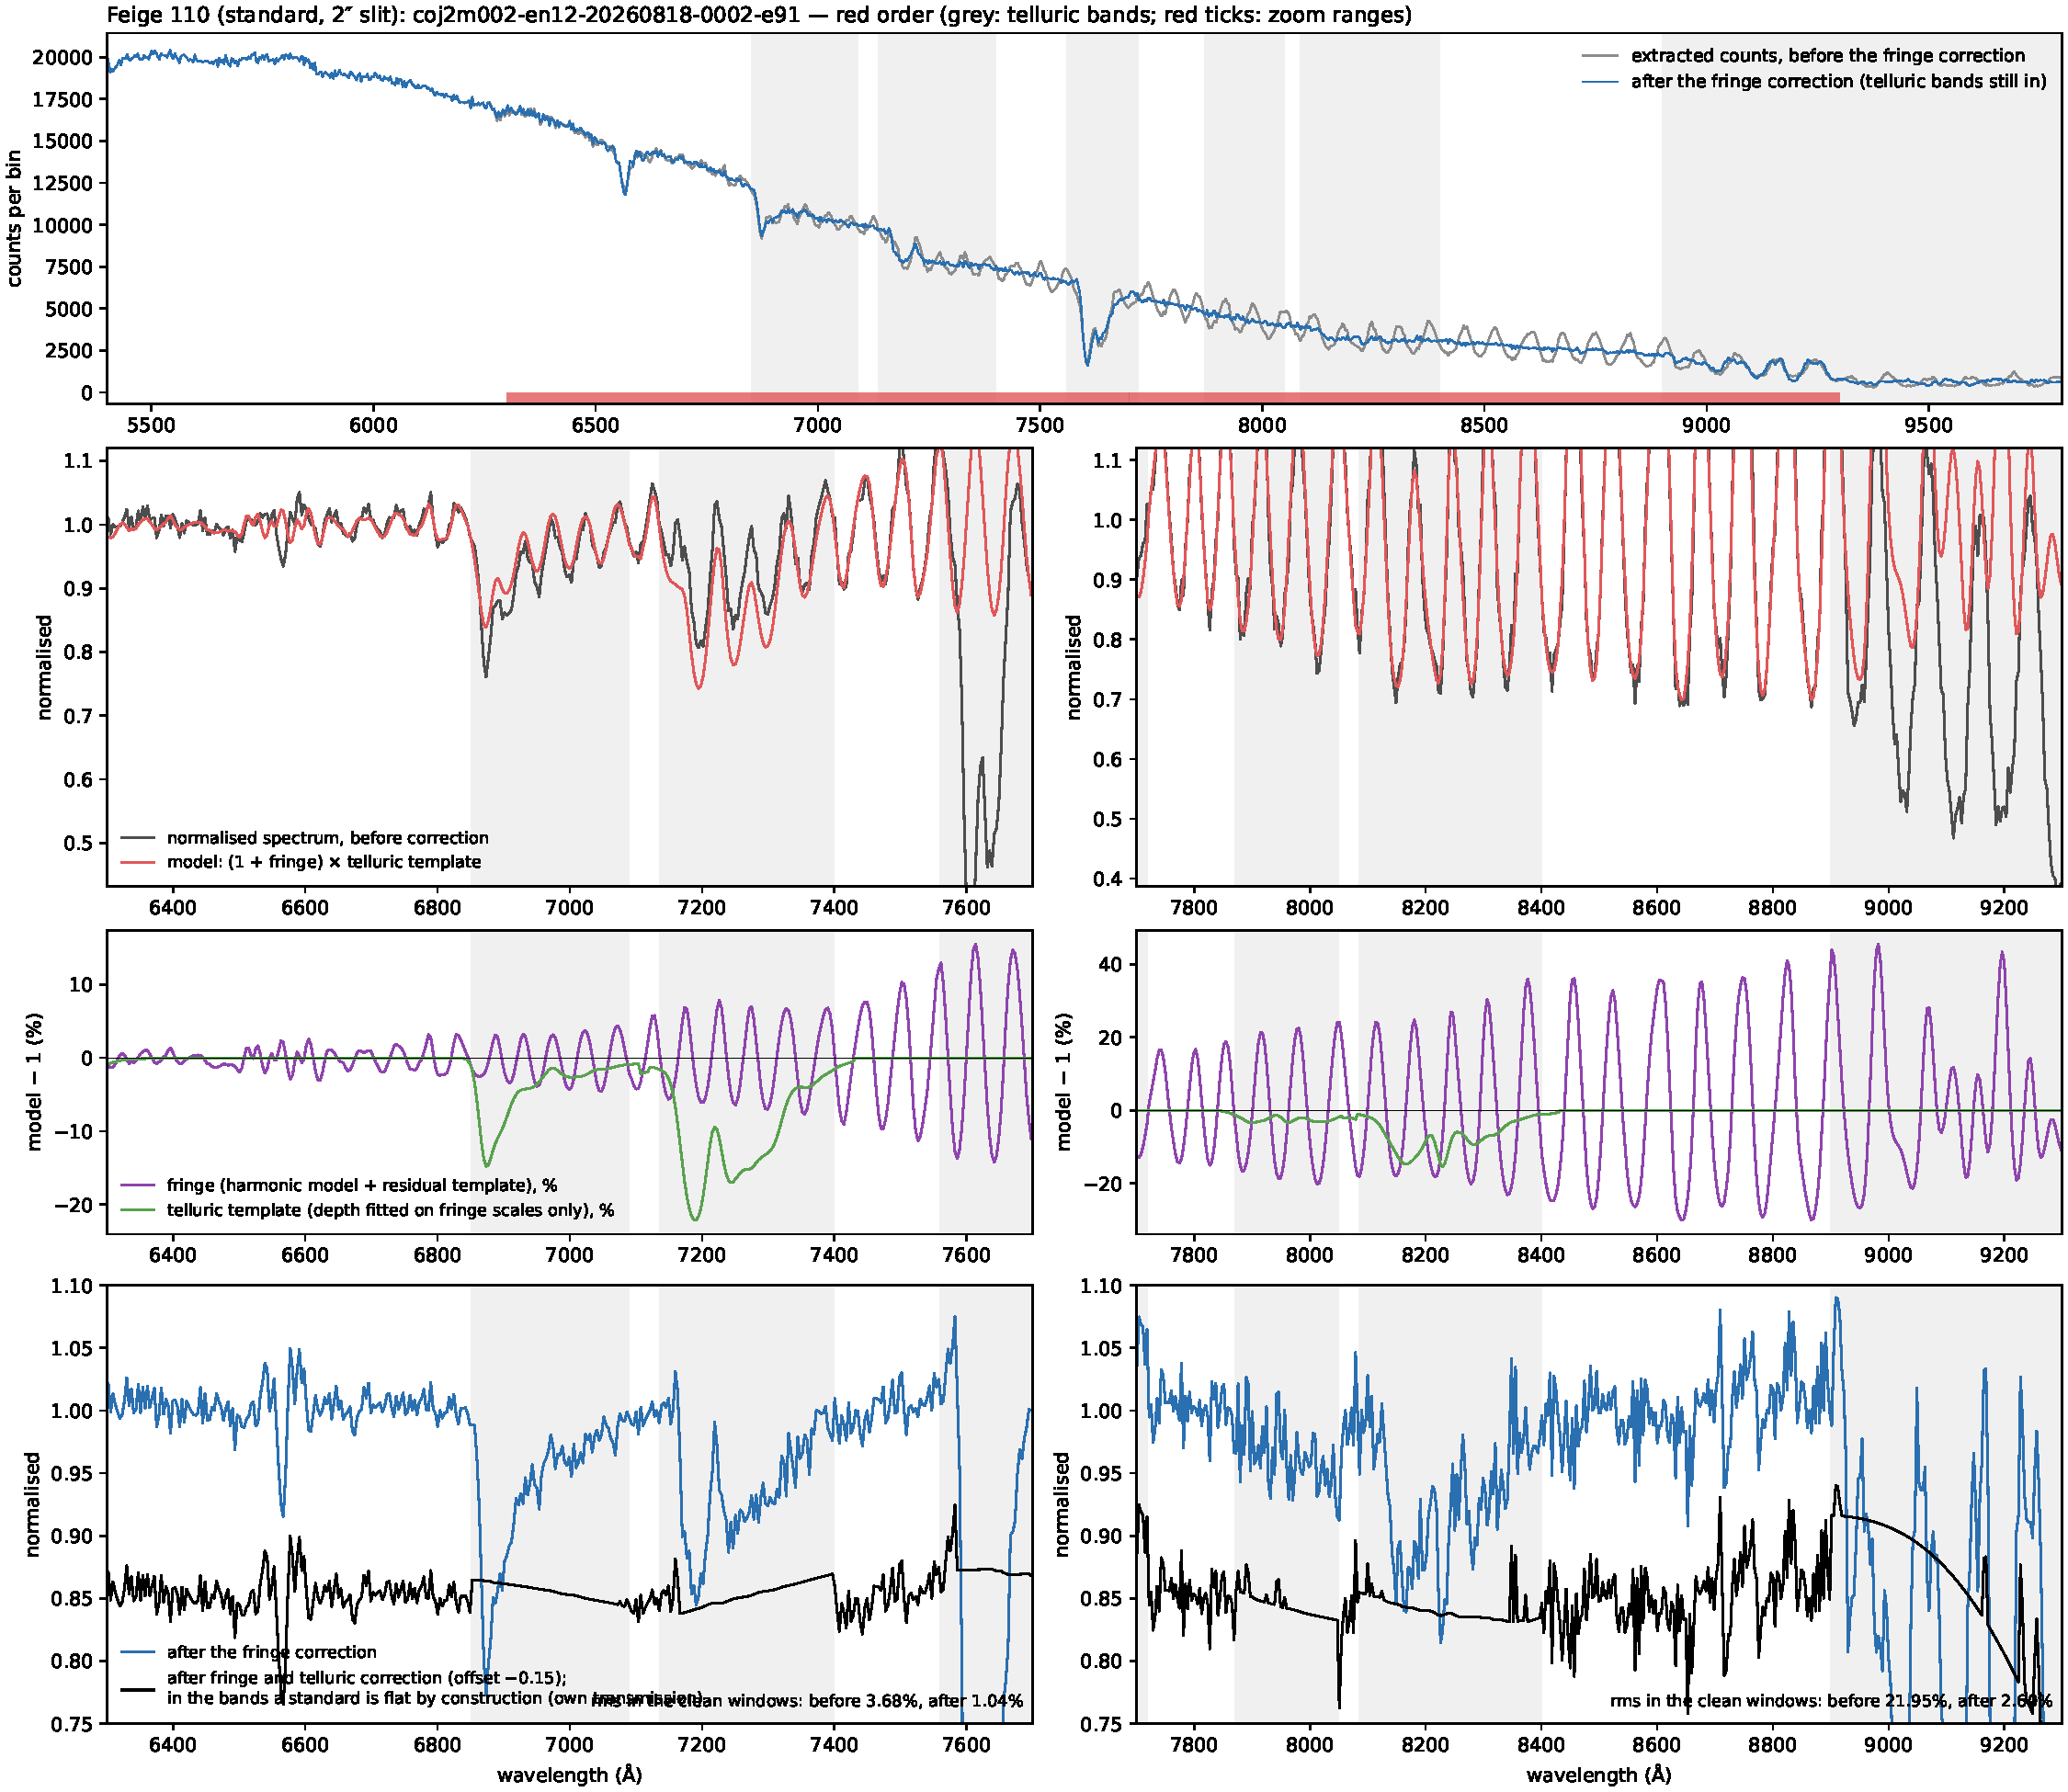
\includegraphics[width=\textwidth]{figures/fig_fringe_example_standard.pdf}
\caption{Fringe + telluric correction of the Feige\,110 exposure 2026-08-04 \#21 (fringe-fit residual 0.21; median of
the 39 exposures 0.26), at 6300--7700\,\AA{} (left) and 7700--9300\,\AA{} (right); grey shading: telluric bands. Top:
the normalised spectrum before correction (grey; counts over the reference at the FLOYDS resolution, over a smooth
continuum) and the fitted model. Middle: the same spectrum after the fringe and telluric correction (v3), with the
rms in the clean windows before $\to$ after. Bottom: the two model components, the fringe (including the residual
template of the slit) and the telluric template, whose depth is constrained only on fringe scales. Inside the bands
the corrected standard is smooth by construction, since its own transmission is measured there. The exposure with
the median residual can no longer be refitted (its 2-d pixel table was removed when the products were made lean,
Section~\ref{sec:sites_disk}); this is the nearest of the frames that keep it.}
\label{fig:fringe_example_std}
\end{figure}

\begin{figure}[!htbp]
\centering
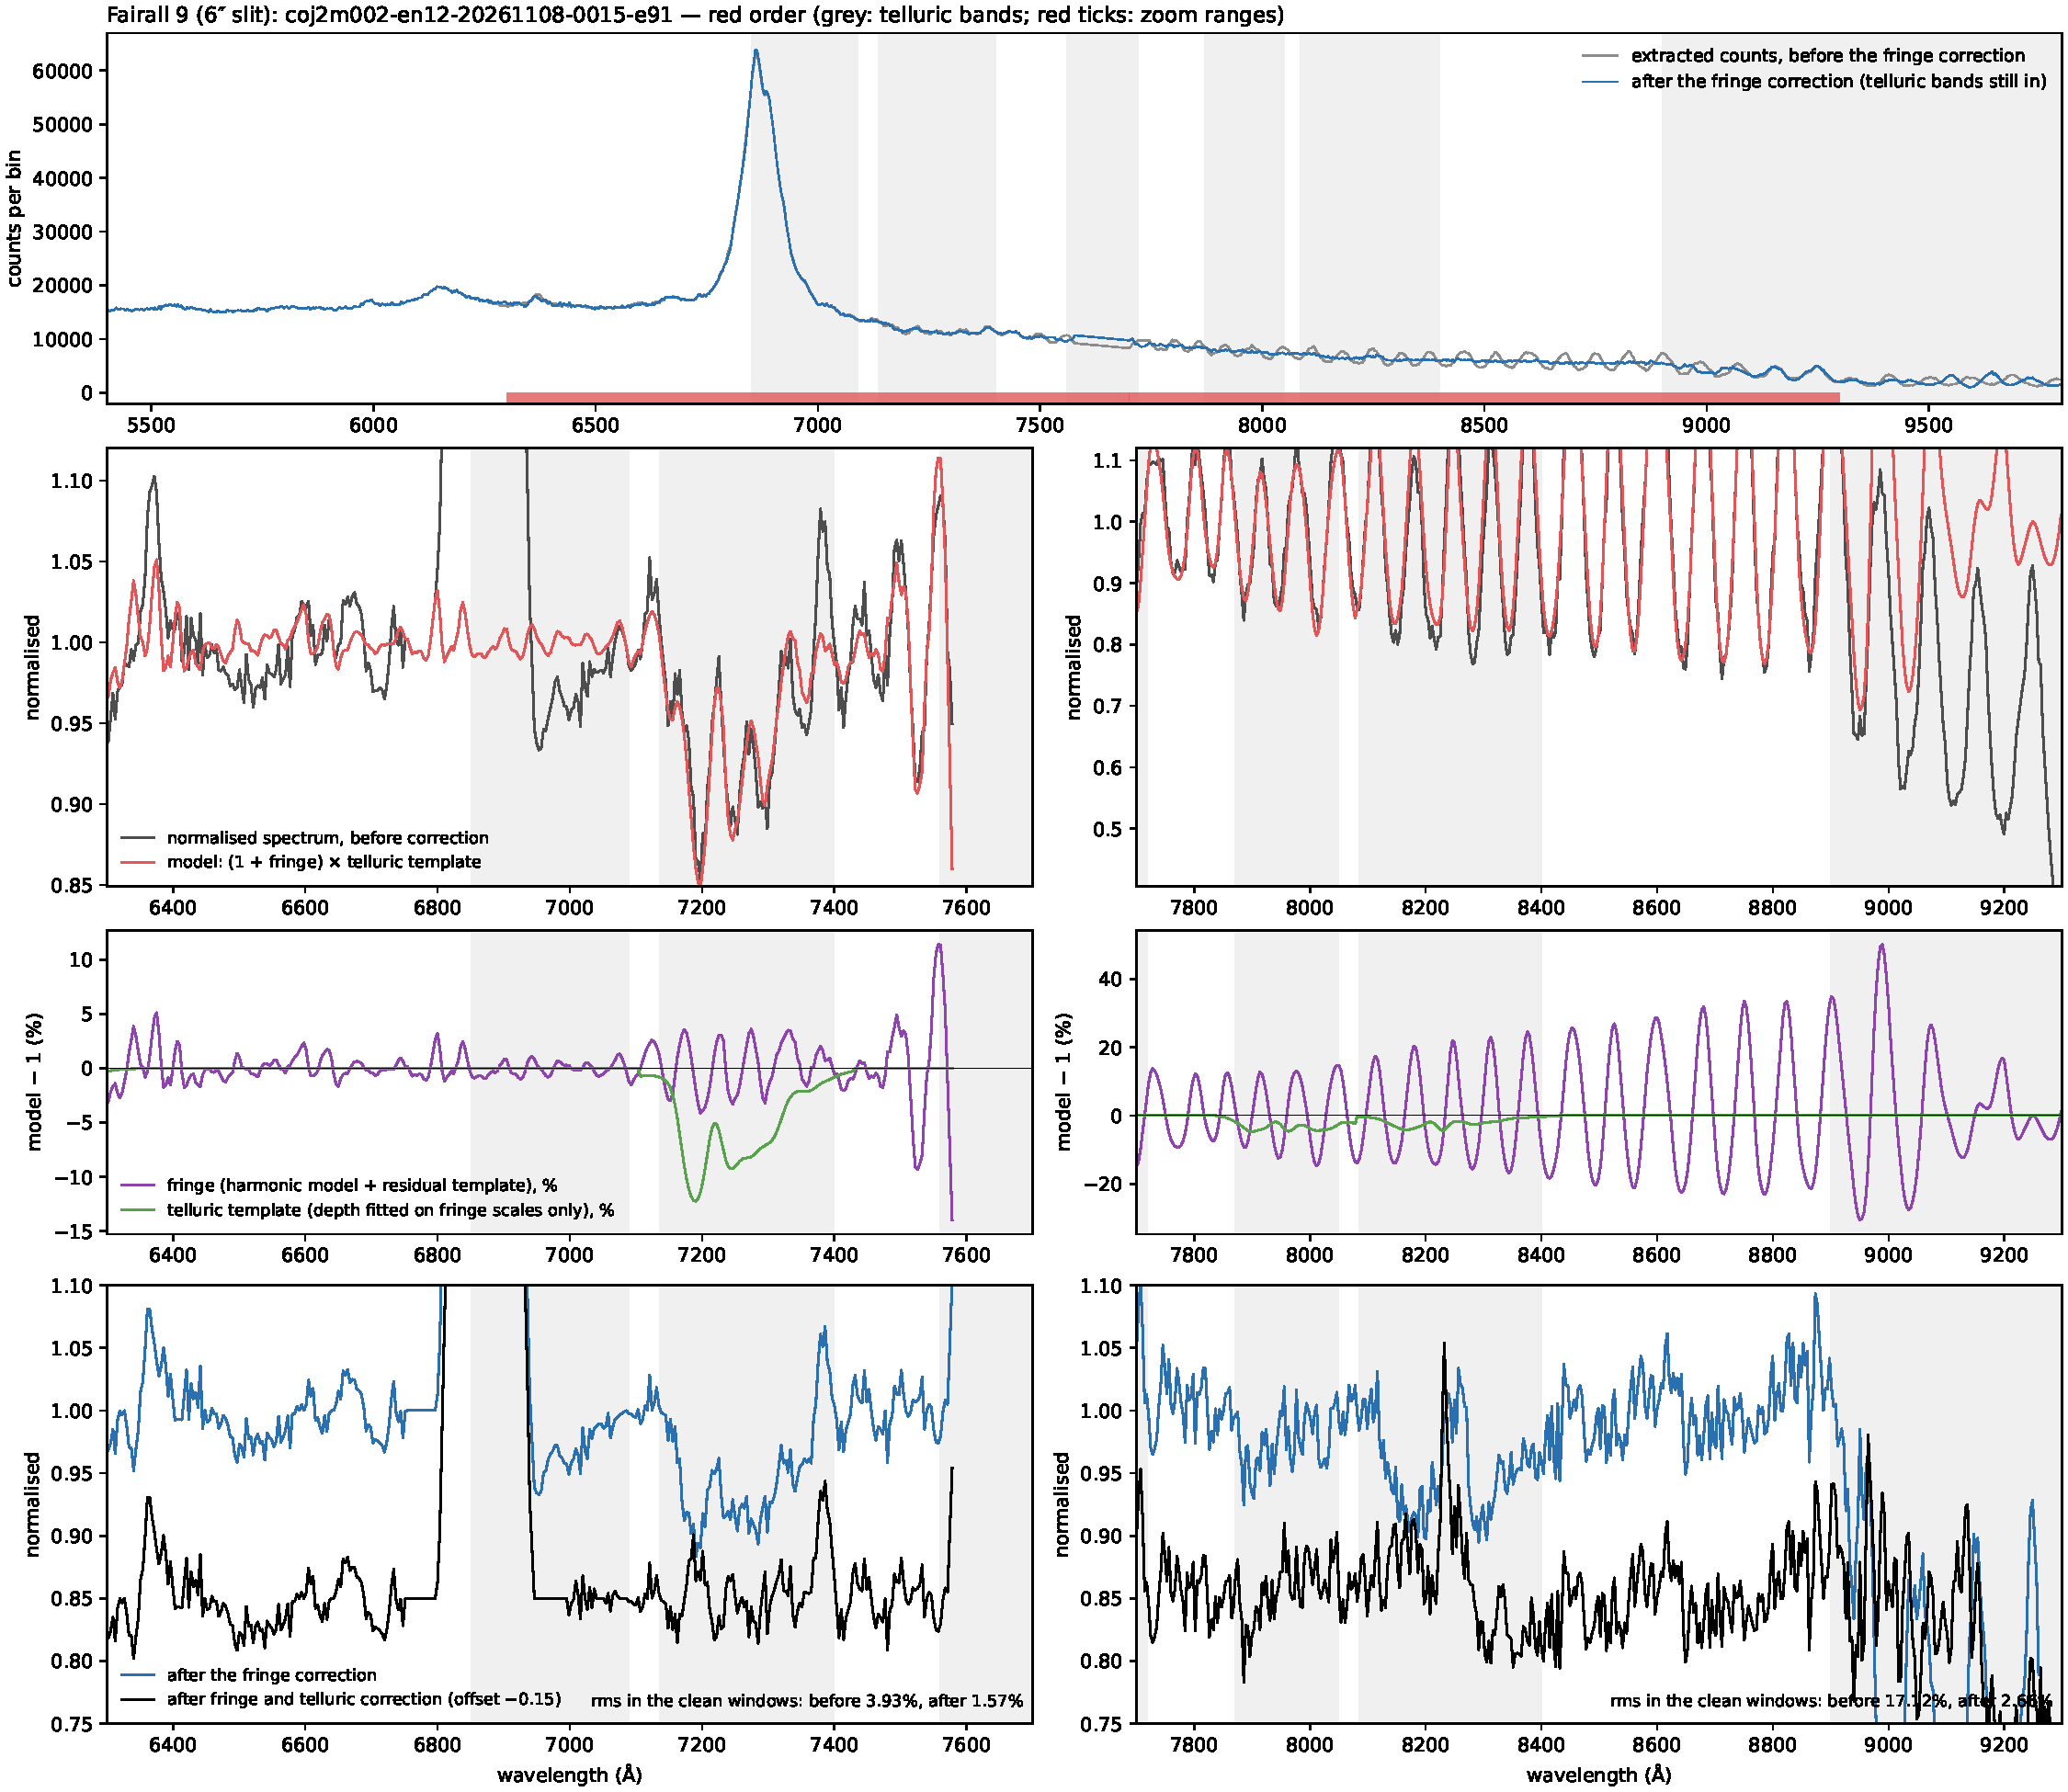
\includegraphics[width=\textwidth]{figures/fig_fringe_example_f9.pdf}
\caption{As Fig.~\ref{fig:fringe_example_std} for the Fairall~9 exposure 2026-08-28 \#9 (6\,arcsec slit), normalised
by a smooth continuum of the corrected spectrum (no reference: the AGN lines remain). The telluric correction of a
science frame is the median transmission of the nine nearest standards scaled to its airmass. Only two Fairall~9
frames keep the 2-d pixel table the refit needs; both are among the worst 5 per cent in the level of the
8110--8380\,\AA{} water band (this one ranks 96 of 100), which shows in the right-hand panels.}
\label{fig:fringe_example_f9}
\end{figure}

The 6300--7700\,\AA{} region is now inspected star by star in every assessment of the fringe correction
(Fig.~\ref{fig:zoom}, Section~\ref{sec:raw_compare}).

\chapter{Flux calibration}
\label{sec:flux}

\section{How \banzai{} selects and uses standards}
\label{sec:flux_banzai}
\banzai{} selects the flux standard in this order: the same observing block; otherwise the closest in time from the
same proposal; otherwise any public standard. Standards are \emph{not} matched by slit width. The Fairall~9 frames
therefore used the eight 6\,arcsec standards taken by the RM proposal between 2026 September 22 and October 8, and
every frame after October 8 used the October 8 standard, although a 2\,arcsec EG\,21 spectrum from LCO's standards
programme exists on most nights. EG\,21 is, moreover, absent from \banzai's flux-standard catalogue (which lists
GD\,108, EG\,274, Feige\,110, Feige\,34 and BD$+28^\circ4211$), so the 18 EG\,21 observations never produced a
sensitivity function and were themselves calibrated with the October 8 standard. The red-order sensitivity of the
October 3 standard has a spike ($+20/-5$ in $\ln S$) at 5200\,\AA. In 1.0.1 the sensitivity is a B-spline in $\ln S$
with fine knots, which also follows the fringes of the standard (Fig.~\ref{fig:sens}).

\textit{Absolute level of the archive spectra.} The archive Fairall~9 spectra are $2.2\pm0.3$ times brighter than
the same exposures reduced with \banzai{}~1.1.0 (stock) or with improved v3, at all wavelengths and for all epochs (also for the
33 epochs calibrated with the same October 8 standard), while the extracted counts agree to 1--4 per cent and EG\,21
agrees with its reference in all reductions. The cause is the exposure time: in 1.0.1 the sensitivity is the
expected flux of the standard over its \emph{counts}, and \texttt{flux\_calibrate} multiplies the science counts by
it without dividing by any exposure time, so a science frame is scaled by $t_{\rm sci}/t_{\rm std}$ = 600\,s/300\,s
= 2 for Fairall~9 (the remaining $\approx10$ per cent is the 1.0.1 sensitivity itself, a Savitzky--Golay filter of
expected over observed counts). EG\,21 (300\,s, like the standards) is unaffected. 1.1.0 uses count rates, and the
improved v3 agrees with \banzai{}~1.1.0 (stock) to 4 per cent. In the raw headers the October 8 standard
(\texttt{coj2m002-en12-20261008-0001}) is Feige\,110 through the 2\,arcsec slit. Since all the
standards of the campaign are 2\,arcsec while Fairall~9 is observed through 6\,arcsec, the absolute level of the
final spectra is still biased high by the slit losses of the standards (seeing-dependent; the grey normalisation to
the clearest standards, which have the lowest $S$, keeps the bias at its minimum); RM light curves, which are
scaled to [O\,{\sc iii}], are not affected.

\begin{figure}[!htbp]
\centering
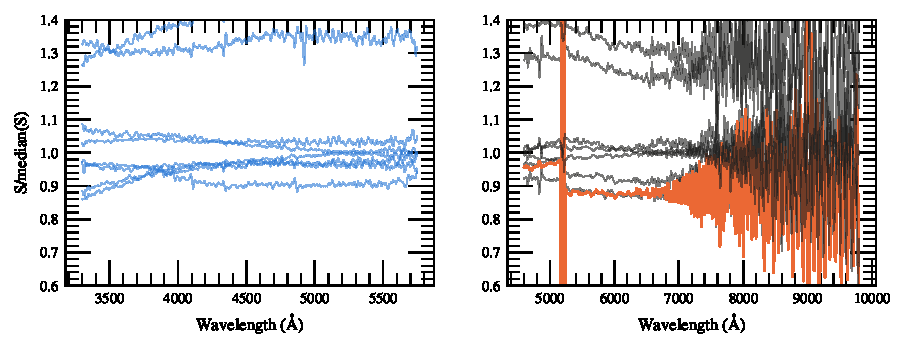
\includegraphics[width=\textwidth]{figures/fig_sens.pdf}
\caption{The eight sensitivity functions used by the archive Fairall~9 spectra, each divided by their median. Orange:
the 2026-10-03 standard (spike at 5200\,\AA). Redward of 7000\,\AA{} the fine-knot fit has learned the fringes of
each standard.}
\label{fig:sens}
\end{figure}


\section{Template $\times$ nightly correction}
\label{sec:flux_model}
Many standards, including EG\,21, have only low-resolution reference fluxes (here the CTIO spectrum in 50\,\AA{} bins;
\citealt{Hamuy1992,Hamuy1994}), which cannot resolve the instrumental notches of the blue order (50--150\,\AA{} wide).
We therefore write the sensitivity of night $n$ and order $o$ as
\begin{equation}
S_{n,o}(\lambda)=T_o(\lambda)\,\exp\left[\sum_{k=0}^{4}p_{n,o,k}\,L_k(\tilde\lambda)\right],
\label{eq:sens}
\end{equation}
where the template $T_o$ carries the fine structure and the Legendre series the smooth, night-dependent part. $T_{\rm
blue}$ is the median of the eight 6\,arcsec sensitivities of \banzai{} (each grey-normalised); $T_{\rm red}$ is the
median of the six good ones smoothed with a 401\,\AA{} running median (no fine structure is needed in the red once
the fringes are removed in the extraction). With $C(\lambda)$ the count rate of the standard corrected for
extinction,
\begin{equation}
C(\lambda)=\frac{N(\lambda)}{t_{\rm exp}\,\tau(\lambda,X)},
\label{eq:rate}
\end{equation}
\begin{equation}
\tau(\lambda,X)=\left[10^{-0.4\,k(\lambda)}\right]^{X\exp[-(h-2788\,{\rm m})/10\,400\,{\rm m}]},
\label{eq:ext}
\end{equation}
($k$ the APO extinction curve shipped with \banzai, $h=1149$\,m for COJ), the coefficients $p_{n,o,k}$ are fitted
to
\begin{equation}
y_j=\ln\frac{F^{\rm ref}_j}{\langle C\,T_o\rangle_j}
\label{eq:sensfit}
\end{equation}
in the reference bins $j$ ($\langle\cdot\rangle_j$ the mean over the bin, required to be $\ge80$ per cent populated),
excluding bins overlapping telluric bands or the cores ($\pm40$\,\AA) of the Balmer lines, with iterative $3\sigma$
clipping.

\textit{Quality control and grey level.} For each order the fitted $P_n(\lambda)$, after removing its median, is compared
with the median over all standards on a grid; a standard deviating by more than $4\times\max(\mathrm{MAD}\times1.4826,
0.02)$ anywhere is rejected. Clouds during the standard exposure raise $S=F^{\rm ref}/C$ grey-ly; to keep the nightly
shape without transferring the standard's clouds, each standard's sensitivity (both orders) is multiplied by
$\exp(\bar g-g_n)$, with $g_n$ the median of $\ln S_{n,{\rm red}}$ at 5500--6500\,\AA{} and $\bar g$ the median of $g_n$
over the clearest (lowest-$g$) half of the standards.

\section{Ensemble flux calibration in the pipeline}
\label{sec:flux_ensemble}
In the reduction from raw the grey normalisation and the ensemble are part of \texttt{FluxCalibrator}
(\texttt{FLUX\_ENSEMBLE\_DAYS}, \texttt{FLUX\_ENSEMBLE\_N}). Each standard still gets its own sensitivity from the
1.1.0 stage \texttt{FluxSensitivity} (a B-spline in $\ln S$ with knots every 20\,\AA{} blueward of 6500\,\AA{} and
every 600\,\AA{} redward, fitted after the harmonic fringe correction). A science frame then uses, instead of the
sensitivity of the single nearest standard, the median of the sensitivities of the nine standards nearest in time
(within $\pm90$\,d), each first multiplied by $\exp(\bar g-g_n)$ as above, with $\bar g$ the median level of the
clearest half of those nine (\texttt{FLUX\_GREY\_WINDOW}, \texttt{FLUX\_GREY\_CLEAR\_FRACTION}). The same nine
standards provide the telluric transmission (Section~\ref{sec:flux_tell}). The grey levels of nine consecutive
Feige\,110 exposures typically span a factor of two, i.e.\ clouds during the 300\,s standard were otherwise
transferred to the science. The template of eq.~\ref{eq:sens} is not needed with Feige\,110, whose reference is
sampled every 2\,\AA; it remains the method for standards with coarse references such as EG\,21. The frame header
records the number of standards and the spread of their grey factors (\texttt{L1FLXNST}, \texttt{L1FLXGRY}).

\section{Telluric correction and application}
\label{sec:flux_tell}
The telluric transmission is measured on the same standard: the calibrated standard $C\,S$ is fitted outside the
bands with a smoothing spline $\mathcal{C}(\lambda)$ in $\ln$, and $t(\lambda)=C\,S/\mathcal{C}$ inside the bands
(clipped to $[0.02,1]$; $t=1$ outside). A science frame at airmass $X_{\rm s}$ calibrated with a standard at $X_\star$
is then
\begin{equation}
F_\lambda=\frac{N(\lambda)\,S(\lambda)}{t_{\rm exp}\,\tau(\lambda,X_{\rm s})\,t(\lambda)^{X_{\rm s}/X_\star}},
\label{eq:apply}
\end{equation}
By default $S$ and $t$ are the medians over all good standards of $S_n$ (grey-normalised) and of $t_n^{1/X_{\star,n}}$
(then raised to $X_{\rm s}$); the standard closest in time can be used instead. The median transfers better between
nights (Section~\ref{sec:results_flux}): the smooth part of a single 2\,arcsec standard partly reflects that night's
slit losses, which do not apply to another night or to a 6\,arcsec spectrum. Because RM inter-calibration removes
grey factors, all comparisons below are made on spectral \emph{shapes} unless stated otherwise.


\textit{The telluric model in the pipeline.} \banzai{}~1.1.0 measures the transmission on the standard in broad
regions that together cover almost the whole red order (6400--7500, 7800--8690 and 8730--9960\,\AA) and divides
every science spectrum by it. Outside the real absorption bands this ratio is the standard's noise and residual
structure: its 12/150\,\AA{} high-pass has an rms of 0.9--1.1 per cent at 6960--8050\,\AA{} and 3 per cent at
8450--8900\,\AA, and it reappears unchanged in every science spectrum, where it was the main remaining source of
fringe-like bumps at 6500--7500\,\AA{} after the harmonic fringe correction. Applying the transmission only in the
absorption bands (\texttt{TELLURIC\_MODEL\_BANDS}) lowers the high-pass rms of the Fairall~9 spectra from 3.4 to 3.0 per cent at
6400--6850\,\AA{} and from 4.3 to 3.4 per cent at 8450--8900\,\AA. For a science frame taken through the same slit as
the standard (EG\,21 with the 2\,arcsec Feige\,110 standards) the broad division is slightly better (0.9 against
1.0 per cent at 6960--7150\,\AA), because part of the residual structure belongs to the slit configuration and
cancels; for 6\,arcsec RM spectra calibrated with 2\,arcsec standards it does not.
The bands are where the Matheson et al.\ (2000) transmission at 9\,\AA{} resolution is more than 1 per cent below
unity: 6850--7090 (O$_2$ B band), 7135--7400 (H$_2$O), 7560--7720 (O$_2$ A band), 7870--8050 and 8085--8400
(H$_2$O) and 8900--9900\,\AA. A first choice that stopped at the band cores (6860--6960, 7150--7350 and
8100--8380\,\AA) left the wings uncorrected: a 1--2 per cent deficit at 6960--7090 and 7350--7400\,\AA, conspicuous
in the flux-calibrated standards (Fig.~\ref{fig:zoom}).

\textit{The O$_2$ A band.} In the 6\,arcsec Fairall~9 spectra the saturated A band (7590--7700\,\AA) leaves a residual
common to all spectra, +25 per cent at the band head and $-17$ per cent at 7620\,\AA{} (10 per cent rms of the median
over spectra), while in EG\,21, taken through the same 2\,arcsec slit as the standards, it is 1.7 per cent
(Fig.~\ref{fig:aband}). The transmission measured through the 2\,arcsec slit resolves the band head differently
from a 6\,arcsec spectrum, and the fringes (10--12 per cent there) are interpolated across the band in both. Sky lines
cannot provide the line-spread function of the object: they fill the slit ($\sigma=35$\,\AA{} through 6\,arcsec
against 6.7\,\AA{} through 2\,arcsec). Broadening the transmission by a fixed $\sigma=5$\,\AA, or by a width fitted to
each frame's own A band or to its water band, lowers the per-spectrum residual of Fairall~9 only from 8.4 to 7.8, 6.4
(fitted on the A band itself, an optimistic bound) and 8.0 per cent. The band is therefore flagged in the science
spectra: 7580--7700\,\AA{} carries bit 2 in the \texttt{mask} column (\texttt{TELLURIC\_FLAG\_BANDS}; header
\texttt{L1TELFLG}); the flux values are kept.

\begin{figure}[!htbp]
\centering
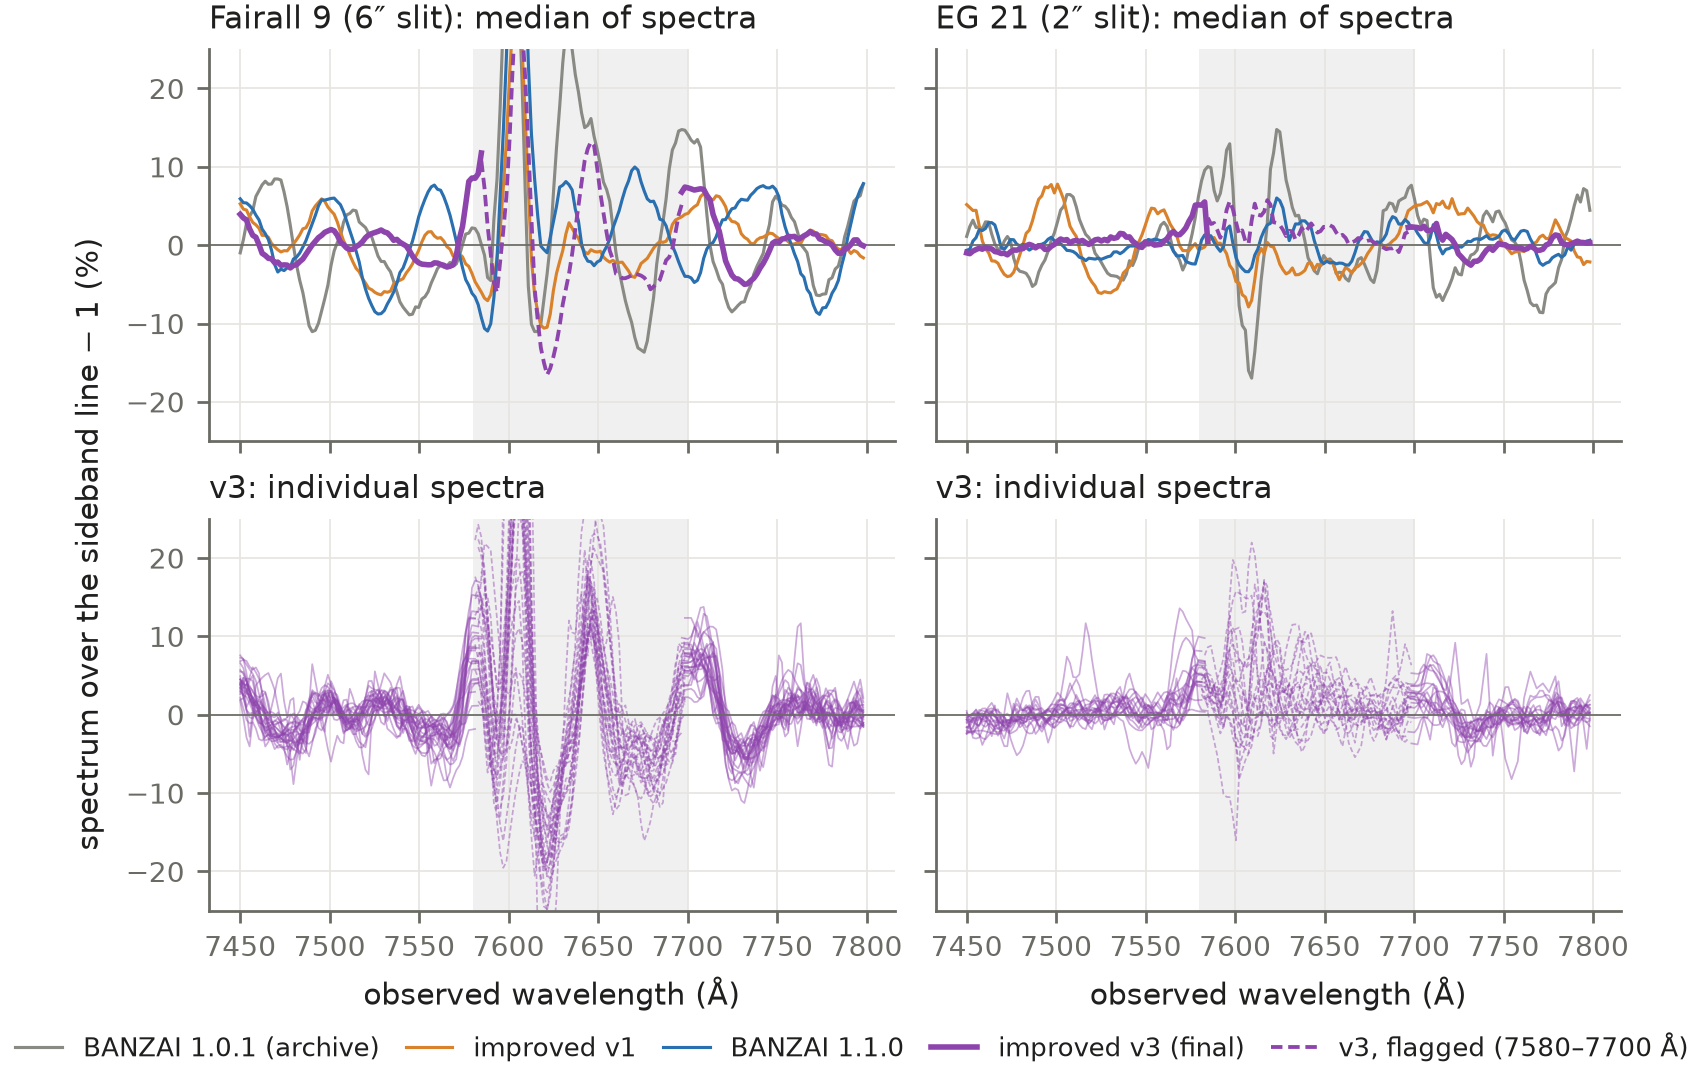
\includegraphics[width=\textwidth]{figures/fig_aband.png}
\caption{The O$_2$ A band: each spectrum over a straight line through the sidebands (7450--7545 and
7735--7800\,\AA). Top: median over spectra for the reductions; bottom: individual spectra of improved v3. Left:
Fairall~9 (6\,arcsec); right: EG\,21 (2\,arcsec, as the standards).}
\label{fig:aband}
\end{figure}
Inside the bands, the transmission of a single standard carries that standard's noise; the pipeline therefore
uses, for science frames, the median over the nine standards nearest in time (within 90\,d) of the transmission
reduced to unit airmass, $t_n^{1/X_n}$, raised to the airmass of the frame (\texttt{TELLURIC\_ENSEMBLE\_N},
\texttt{TELLURIC\_ENSEMBLE\_DAYS}), as in the archive-based recalibration (Section~\ref{sec:flux_tell}). This
lowers the scatter between the Fairall~9 spectra at 7000--7500\,\AA{} from 1.73 to 1.63 per cent. Inside the
water bands a residual of 4 per cent remains (7170--7330 and 8130--8360\,\AA, against 1.8 and 3.2 per cent in the
archive-based recalibration): it is common to the standards, so the median does not remove it. We attribute it to
the fringes of the standards themselves inside the bands, which the pipeline's harmonic fit of a standard
interpolated across the masked bands instead of fitting; the archive-based recalibration refitted them on the
telluric-corrected spectra. The joint fringe and telluric fit (Section~\ref{sec:fringe_joint}) solves this: in
improved v3 the water-band residuals of Fairall~9 are 1.7 and 3.2 per cent, as in the archive-based recalibration
(Table~\ref{tab:versions}).

\section{Results}
\label{sec:results_flux}
The small-scale scatter between the spectra (Fig.~\ref{fig:series}, Table~\ref{tab:summary}) improves in every red
region (by factors of 1.3--2.2) and slightly in the blue. The [O\,{\sc iii}] flux, which should be constant, scatters
less in both orders, and the red/blue [O\,{\sc iii}] flux ratio -- a direct test of the relative calibration of the two
orders -- improves from \FRBOld{} to \FRBOpt{} (optimal) and \FRBBox{} (boxcar) per cent. Normalising the grey level of
the nightly standards to the clearest nights is essential: without it the clouds at the time of the (300\,s) standard
exposure are transferred to the science and the blue [O\,{\sc iii}] scatter rises to 20 per cent. A standard taken in
7\,arcsec seeing through the 2\,arcsec slit initially gave a broken extraction (the object mask left 13 sky pixels);
the adaptive sky mask and the bounded cosmic-ray rejection (Section~\ref{sec:extraction}) fix it, and the
shape-deviation test (Section~\ref{sec:flux_model}) would reject such a standard otherwise.

The closure test on EG\,21 (Fig.~\ref{fig:standard}) measures how well a sensitivity transfers between nights: each
EG\,21 spectrum is calibrated with the median of the other 17. The shape scatter against the CTIO reference is
\CLbNew{} (blue) and \CLrNew{} per cent (red), compared with \CLbOld{} and \CLrOld{} for the archive spectra calibrated
with a single 6\,arcsec standard. Calibrating each night with the nearest other night's standard instead is worse
(1.8 and 2.7 per cent): the smooth part of a single 2\,arcsec standard carries that night's slit losses. On the
archive extractions, a same-night standard gives 0.7 and 1.5 per cent and matters most below 3800\,\AA{} (0.5 against
3--5.5 per cent from another night), so a same-night standard of the science's own slit width remains the best option
when it exists. The EG\,21 nights themselves have a stable 2\,arcsec response: the smooth part varies by
0.5--1.2 per cent (2--2.5 per cent at the ends) and the tilt by 1.3--1.4 per cent per 1000\,\AA{} (weakly seeing
dependent); a 2\,arcsec standard can therefore calibrate 6\,arcsec science to $\approx1$--2 per cent in shape.

\begin{figure}[!htbp]
\centering
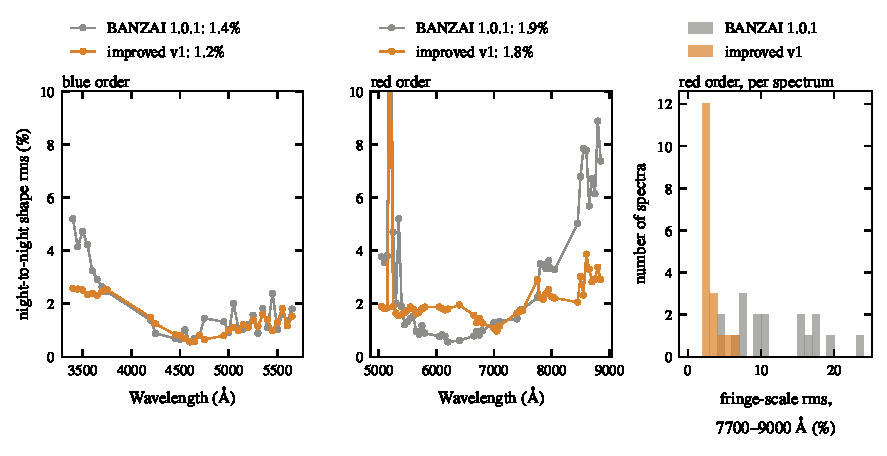
\includegraphics[width=\textwidth]{figures/fig_standard.pdf}
\caption{EG\,21 closure test. Left and middle: night-to-night rms of the shape of the 18 calibrated EG\,21 spectra
relative to the CTIO reference in its 50\,\AA{} bins (telluric and Balmer bins masked): archive (grey) and this work
(each night calibrated with the median sensitivity of the other 17 nights). Right: fringe-scale rms of the red order.}
\label{fig:standard}
\end{figure}



\chapter{Running \banzai{} from the raw frames}
\label{sec:raw}

The corrections of Chapters~\ref{sec:traces}--\ref{sec:flux} were first developed on the archive products, undoing
parts of the archive processing where necessary (Appendix~\ref{sec:app_v1}). Running the pipeline from the raw frames
removes the need to undo anything:
the destroyed pixels are not created, the 2-d frame is resampled once on the corrected wavelength grid, the
uncertainties are propagated from read noise and photon counts, and standards and science are treated identically. It
also gives the collaboration a reproducible pipeline for new data. This chapter describes the offline set-up, the
\banzai{}~1.1.0 (stock) run that serves as the baseline, and the comparison of the five reductions
(Table~\ref{tab:versions_names}).

\section{Data and calibration database}
\label{sec:raw_data}
The raw data set (Table~\ref{tab:rawdata}) contains 100 Fairall~9 exposures in 50 blocks of two consecutive
exposures on 47 nights (2026 August 28 -- November 11); every block has its own arc and lamp flat. The 57 standard-star
exposures are all through the 2\,arcsec slit: Feige\,110 (39, in the \banzai{} standards catalogue, with a finely
sampled reference spectrum) and EG\,21 (18). Forty of the 47 Fairall~9 nights have a standard (Feige\,110 on 25, EG\,21
on 15); the nearest standard is a median of 1.5\,h from the science block, within 3\,h for 33 of the 50 blocks.

\begin{table}[!htbp]
\centering
\caption{Raw frames used for the reduction from raw. All from \texttt{coj2m002-en12}.}
\label{tab:rawdata}
\begin{tabular}{lccc}
\toprule
Frames & Slit & $N$ & With an arc and a lamp \\
 & (arcsec) & (frames) & flat in the same block \\
\midrule
Fairall~9 & 6 & 100 (50 blocks, 47 nights) & 100 \\
Feige\,110 & 2 & 39 & 38 \\
EG\,21 & 2 & 18 & 18 \\
Arcs & 6 / 2 & 64 / 58 & -- \\
Lamp flats & 6 / 2 & 69 / 64 & -- \\
Sky flats (2025 December 8) & 1.2, 1.6, 2, 6 & 4 & -- \\
\bottomrule
\end{tabular}
\end{table}

\banzai{} (version 1.1.0 of this checkout, i.e. newer than the 1.0.1 that produced the archive) runs offline with a
local SQLite calibration database. The set-up (scripts in \texttt{work/banzai\_run}) creates the sites and
instruments, loads the order heights and locations, the line-spread-function parameters and the flux standards
shipped with the package, and processes the four sky flats (relabelled as \texttt{SKYFLAT}, as the package's own
calibration notebook does). Their order traces reproduce the archive \texttt{ORDER\_COEFFS} to $\leq0.7$\,px; the
difference reflects the changes to the order fitting between 1.0.1 and 1.1.0. The frames are then reduced in the
order arcs, lamp flats, standards and science, each with \texttt{run\_pipeline\_stages}, so that every frame can find
its calibrations in the database. EG\,21 is not in the catalogue and is reduced as a science frame.

\section{Processing time}
\label{sec:raw_time}
All 412 raw frames were reduced without failures on a laptop (8 cores, 8\,GB of memory), four frames in parallel.
Table~\ref{tab:timing} gives the wall-clock time per frame. Arcs dominate: the 2-d wavelength solution of an arc takes
$\approx48$\,s ($\approx34$\,s since the faster line fits of Section~\ref{sec:visit_timing}), against 4\,s for a lamp flat and 11--16\,s for a science or standard exposure. With improved v3 a
science exposure takes 10\,s, because it no longer searches for the shift of the fringe pattern along the slit in the
2-d frame. Section~\ref{sec:visit_timing} gives the time per visit and per pipeline stage for improved v3, and the
projection to a decade of data.
Disk space matters as much as processor time. A processed 2-d frame is 47\,MB, of which 43\,MB is the uncompressed
table of individual pixels (\texttt{BINNED2D}). A decade of data therefore needs either fewer products written per
frame or compressed tables.

\begin{table}[!htbp]
\centering
\caption{Processing time per frame (wall-clock, four frames in parallel on an 8-core laptop).}
\label{tab:timing}
\begin{tabular}{lccc}
\toprule
Frame type & $N$ & median time & total, 4 workers \\
 & (frames) & (s) & (min) \\
\midrule
Arc & 122 & 48 & 26 \\
Lamp flat & 133 & 4 & 3 \\
Standard (Feige\,110) & 39 & 16 & 3 \\
Science (Fairall~9, EG\,21) & 118 & 11 & 6 \\
Science, improved v3 & 118 & 10 & 6 \\
Standard, improved v3 (two passes) & 39 & $2\times12$ & 4 \\
\bottomrule
\end{tabular}
\end{table}


\section{Processing time per visit}
\label{sec:visit_timing}
A visit is one block of the campaign: an arc, a lamp flat and the exposures of the target (2 for Fairall~9).
Table~\ref{tab:visit_timing} breaks the processing time of each frame type into the pipeline stages, measured
from the time stamps of the \banzai{} log for the final configuration (one worker; four ran in parallel on an
8-core laptop with 8\,GB of memory). Figure~\ref{fig:visit_timing} adds them up per visit.

\begin{table}[!htbp]
\centering
\caption{Median processing time per frame (s, one worker) by pipeline stage, final configuration. ``Arc'' is
the 2-d wavelength solution; ``orders'' the order loading and tweak; ``fringe'' the lamp-pattern loading and the
harmonic fit (joint with the telluric template); ``flux + telluric'' the sensitivity, the ensemble flux
calibration and the telluric correction; ``other'' reading, writing and database access.}
\label{tab:visit_timing}
\small
\begin{tabular}{lcccccccccc}
\toprule
Frame & $N$ & arc & orders & fringe & trace & bkg+CR & extract & flux+tell & other & total \\
 & (frames) & (s) & (s) & (s) & (s) & (s) & (s) & (s) & (s) & (s) \\
\midrule
Arc & 122 & 46.3 & 0.2 & -- & -- & -- & 1.2 & -- & -- & 48 \\
Lamp flat & 133 & 0.7 & 0.4 & -- & -- & -- & 0.5 & -- & 2.4 & 4 \\
Standard & 39 & 0.5 & 0.3 & 0.9 & 5.4 & 1.9 & 1.5 & 0.8 & -- & 12 \\
Science & 118 & 0.5 & 0.3 & 0.9 & 3.5 & 1.8 & 2.0 & 0.3 & 0.1 & 10 \\
\bottomrule
\end{tabular}
\end{table}

\begin{figure}[!htbp]
\centering
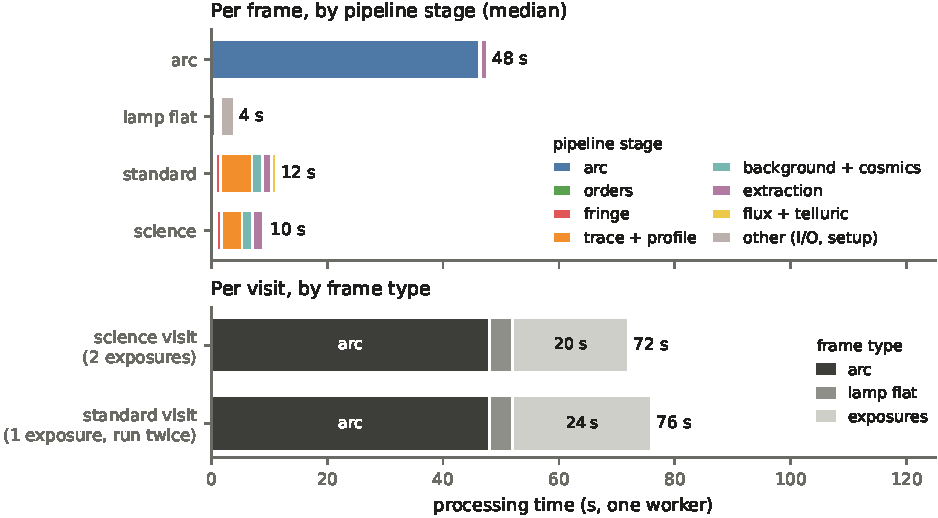
\includegraphics[width=\textwidth]{figures/fig_visit_timing.pdf}
\caption{Left: median processing time per frame by stage. Right: per visit, for a science visit (arc, lamp flat
and 2 exposures) and a standard visit (arc, lamp flat and one exposure, processed twice: before and after the
residual fringe template is measured).}
\label{fig:visit_timing}
\end{figure}

A science visit costs $\approx72$\,s of processing (48\,s arc, 4\,s lamp flat,
2$\times$10\,s for the exposures) and a standard visit $\approx76$\,s. With four workers
the throughput is $\approx18$\,s of wall-clock time per science visit, so the
$\approx5000$ visits of a decade take $\approx25$\,h on this laptop, most of it in the arcs.
Fitting the arc once per instrument epoch and checking each block only for a zero-point shift
(Chapter~\ref{sec:wavelength}) would bring this to $\approx8$\,h. The steps that are not
per frame are small: the fringe phase master of a slit and two-month window takes 3\,s,
the residual fringe template 3\,s, and the ensemble flux and telluric calibrations
read the nearest nine standards from the database for each frame (included in ``flux + telluric'').


\section{Comparison of the reductions: \banzai{}~1.0.1, 1.1.0 and improved v1--v3}
\label{sec:raw_compare}
The five reductions of Table~\ref{tab:versions_names} are compared on the same exposures in
Table~\ref{tab:versions}. Improved v2 and v3 run in \banzai{} from the raw frames; improved v1 is the set of
corrections applied to the archive products. Improved v3 is the final version (Chapter~\ref{sec:sites}). Instead of
refitting the arcs after the reduction, as v1 does, it uses the 1.1.0 arc fit with the added arc lines
(Section~\ref{sec:sites_arcs}), followed by the telluric zero point. Our \banzai{}~1.1.0 run already applies that zero
point, because the stage was already in our copy of the code when the run was made
(Table~\ref{tab:versions_names}). The two runs therefore do not differ in this respect, and the zero point does not
affect any other row of the table.

\begin{table}[!htbp]
\centering
\caption{The same exposures in the five reductions (Fairall~9: the 50 exposures with archive products; EG\,21: 18;
Feige\,110: 39, from raw only). Fringe metric as in Table~\ref{tab:summary}; per-spectrum residual: rms of each red-order spectrum about a fitted
power law (Fig.~\ref{fig:versions_individual}); small-scale scatter between spectra in per cent; [O\,{\sc iii}]
scatters are robust rms in per cent. 6500--7500\,\AA{} and water-band rows: per-spectrum rms of the 12/150\,\AA{}
high-pass (see Conventions) in the clean windows 6620--6850, 6960--7150 and 7350--7550\,\AA, or inside the band
(Fig.~\ref{fig:zoom}). For Fairall~9 the 6500--7500\,\AA{} row gives only the frame-specific part: the median over all
spectra is removed first, which removes the galaxy's narrow lines and anything common to all frames. In Feige\,110, 1.1.0 is low by
construction (each standard is divided by its own observed/expected ratio over most of the red order).}
\label{tab:versions}
\small
\begin{tabular}{lccccc}
\toprule
 & \banzai{}~1.0.1 & \banzai{}~1.1.0 & \multicolumn{3}{c}{improved} \\
Metric & (archive) & (stock) & v1 & v2 & v3 \\
 & (\%) & (\%) & (\%) & (\%) & (\%) \\
\midrule
\multicolumn{6}{l}{\textit{Fairall~9}}\\
Red fringe metric & 13.7 & 8.1 & 2.6 & 2.1 & 1.9 \\
Per-spectrum residual from a power law & 16.9 & 11.2 & 4.9 & 3.7 & 3.4 \\
Blue small-scale scatter 3500--4000\,\AA & 1.61 & 1.32 & 1.44 & 1.37 & 1.33 \\
Blue small-scale scatter 4000--4600\,\AA & 1.84 & 1.49 & 1.64 & 1.49 & 1.47 \\
Blue small-scale scatter 4600--5200\,\AA & 2.00 & 1.64 & 1.82 & 1.64 & 1.64 \\
Blue small-scale scatter 5200--5700\,\AA & 2.78 & 2.37 & 2.60 & 2.35 & 2.31 \\
Red small-scale scatter 5000--6000\,\AA & 2.08 & 0.99 & 1.09 & 0.96 & 0.95 \\
Red small-scale scatter 6000--6800\,\AA & 1.37 & 0.97 & 1.01 & 0.89 & 0.88 \\
Red small-scale scatter 7000--7500\,\AA & 3.18 & 1.94 & 1.65 & 1.63 & 1.35 \\
Red small-scale scatter 7700--8500\,\AA & 7.68 & 3.74 & 2.17 & 2.12 & 1.96 \\
Red small-scale scatter 8500--9500\,\AA & 12.74 & 6.11 & 3.68 & 3.55 & 3.85 \\
{[O\,{\sc iii}]} flux, blue order & 12.7 & 11.2 & 8.8 & 11.1 & 9.8 \\
{[O\,{\sc iii}]} flux, red order & 27.6 & 8.5 & 10.5 & 8.6 & 11.2 \\
Red/blue {[O\,{\sc iii}]} ratio & 29.2 & 8.9 & 9.7 & 8.5 & 6.9 \\
6500--7500\,\AA{} high-pass, frame-specific part & 2.52 & 1.23 & 1.17 & 0.98 & 0.93 \\
Water band 7170--7330\,\AA & 5.84 & 3.22 & 1.71 & 3.85 & 1.71 \\
Water band 8130--8360\,\AA & 16.10 & 7.95 & 3.17 & 4.03 & 3.21 \\
\midrule
\multicolumn{6}{l}{\textit{EG\,21}}\\
Red fringe metric & 9.3 & 2.7 & 2.1 & 1.6 & 1.5 \\
Per-spectrum residual from a power law & 11.7 & 4.0 & 4.2 & 3.0 & 2.5 \\
Red small-scale scatter 7000--7500\,\AA & 3.35 & 1.34 & 1.78 & 1.03 & 1.06 \\
Red small-scale scatter 7700--8500\,\AA & 9.02 & 2.43 & 2.46 & 1.85 & 1.71 \\
Red small-scale scatter 8500--9500\,\AA & 13.13 & 3.56 & 3.40 & 3.07 & 3.01 \\
6500--7500\,\AA{} high-pass & 3.01 & 1.14 & 2.90 & 1.10 & 0.88 \\
Water band 8130--8360\,\AA & 9.96 & 3.31 & 2.93 & 2.78 & 2.23 \\
\midrule
\multicolumn{6}{l}{\textit{Feige\,110 (flux / reference)}}\\
6500--7500\,\AA{} high-pass & -- & 0.68 & -- & 1.22 & 0.97 \\
7750--8900\,\AA & -- & 1.67 & -- & 3.01 & 2.00 \\
\bottomrule
\end{tabular}
\end{table}

Improved v3, run in one pass from the raw frames, has the best fringe correction of all reductions, without having
to undo any earlier processing. The red fringe metric of Fairall~9 is 1.9 per cent (\banzai{}~1.0.1
13.7, 1.1.0 8.1, improved v1 2.6, v2
2.1) and the residual of the individual spectra from a power law
3.4 per cent (Fig.~\ref{fig:versions_individual}). On EG\,21 it is the best in every red
metric but one (small-scale scatter at 7000--7500\,\AA: 1.06 against 1.03 per cent for v2). In the blue order and at 5000--6800\,\AA{} the runs from raw are better than both reductions based on the archive
products, because they have no destroyed pixels and the data are resampled only once. The red/blue [O\,{\sc iii}] ratio, the most
direct test of the relative calibration of the orders, scatters by 6.9 per cent (1.1.0
8.9, v1 9.7, v2 8.5). With the ensemble flux
calibration (Section~\ref{sec:flux_ensemble}) the blue [O\,{\sc iii}] flux scatters by 9.8 per
cent, against 11.2 for 1.1.0 and 11.1 for v2, which both use the single nearest
standard. Improved v1 reaches 8.8 per cent, with an ensemble of the whole campaign rather than of the nine nearest
standards. Inside the water bands v3 matches v1 at 7170--7330\,\AA{} (1.71 against
1.71 per cent) and at 8130--8360\,\AA{} (3.21 against
3.17). The water absorption still changes from night to night ($\approx3.5$ per
cent rms in the level of the 8110--8380\,\AA{} band), and a median of nine standards cannot follow this. The O$_2$ A band
(7580--7700\,\AA) is flagged in the science spectra of v3 (mask bit 2, Section~\ref{sec:flux_tell}).

Figure~\ref{fig:fringe_band} shows the effect of the fringe settings of v3 at 6000--7700\,\AA. In the 18 EG\,21
spectra, the rms of the high-passed spectra in the line- and telluric-free windows drops from 3.91 per cent
(uncorrected) and 0.99 per cent (initial configuration of the pipeline's fringe model) to 0.94 per cent. In all 100
Fairall~9 spectra of the v3 run, the frame-specific part drops from 1.36 per cent (initial configuration) to
0.94 per cent; without any fringe correction it is 1.12 per cent.

Figure~\ref{fig:final_spectra} shows what this means for the spectra themselves: a typical epoch in
\banzai{}~1.0.1 and in improved v3, and the red order of all epochs side by side.

\begin{figure}[!htbp]
\centering
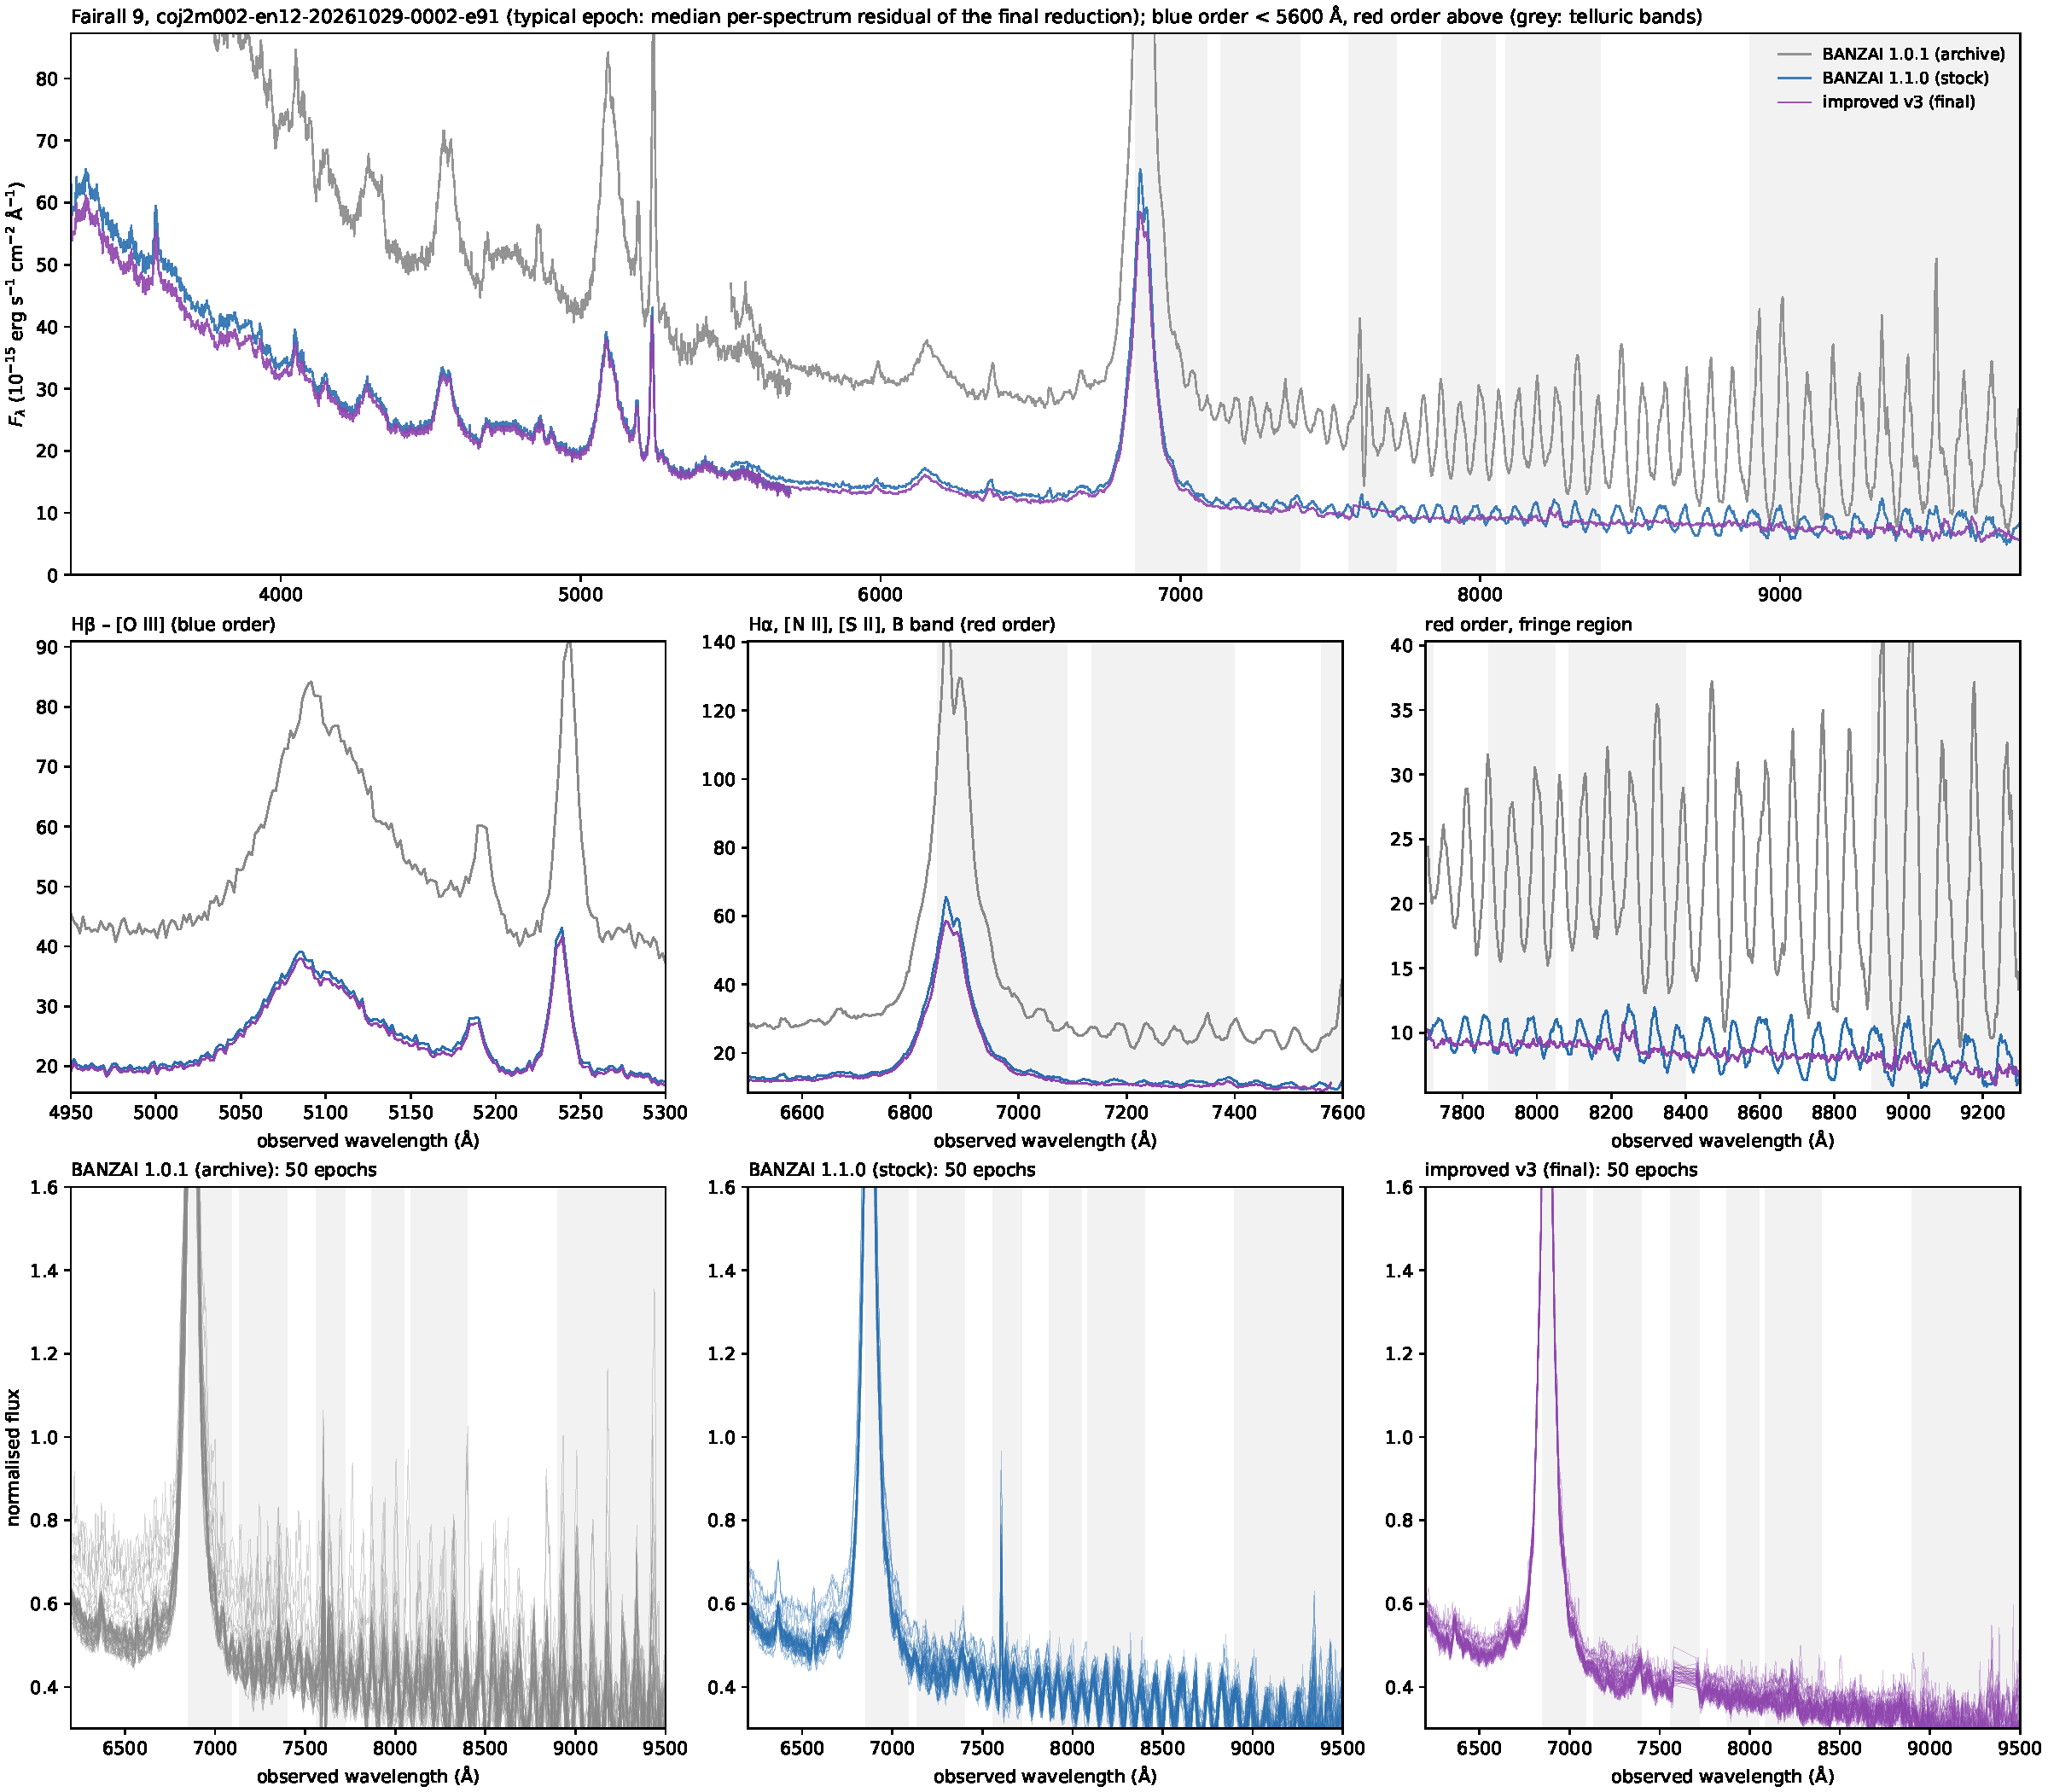
\includegraphics[width=\textwidth]{figures/fig_final_spectra.pdf}
\caption{Fairall~9 in the archive (\banzai{}~1.0.1, grey) and in the final reduction (improved v3, purple). Top: a
typical epoch (median per-spectrum residual of v3), both orders; the archive is multiplied by 0.44, the median ratio of
the two, because 1.0.1 does not divide by the exposure time (Section~\ref{sec:flux_banzai}). Middle: the red end of the
same epoch, where the archive carries the fringes. Bottom: the red order of all 50 epochs with archive products, each
divided by its flux at 5100--5200\,\AA{} (blue order); the spread is the AGN variability plus the calibration errors.
Grey bands: telluric absorption.}
\label{fig:final_spectra}
\end{figure}

\begin{figure}[!htbp]
\centering
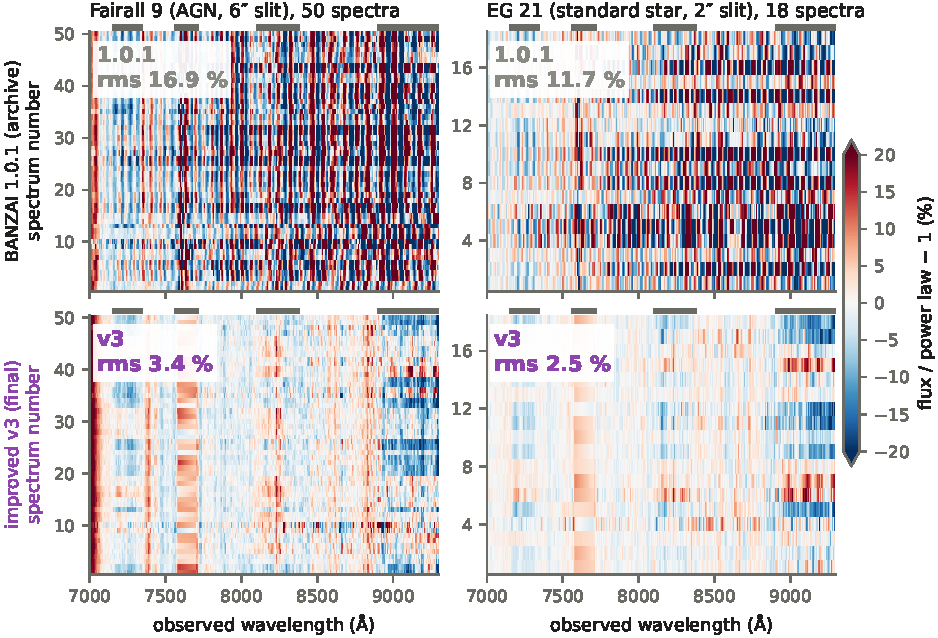
\includegraphics[width=\textwidth]{figures/fig_versions_individual.pdf}
\caption{Every red-order spectrum (one row each, in time order) divided by a power law fitted at 7000--9800\,\AA,
in the archive (\banzai{}~1.0.1, top) and in improved v3 (bottom); Fairall~9 left, EG\,21 right. The vertical stripes
in the archive are the fringes. The rms is the median over spectra in the clean windows 7750--8050 and
8450--8900\,\AA. Grey bars above each panel: telluric bands, left out of the fit. Cut at 9300\,\AA, beyond which the
night-to-night change of the water-vapour absorption dominates; 1.1.0 and v1 are in Table~\ref{tab:versions}.}
\label{fig:versions_individual}
\end{figure}

\begin{figure}[!htbp]
\centering
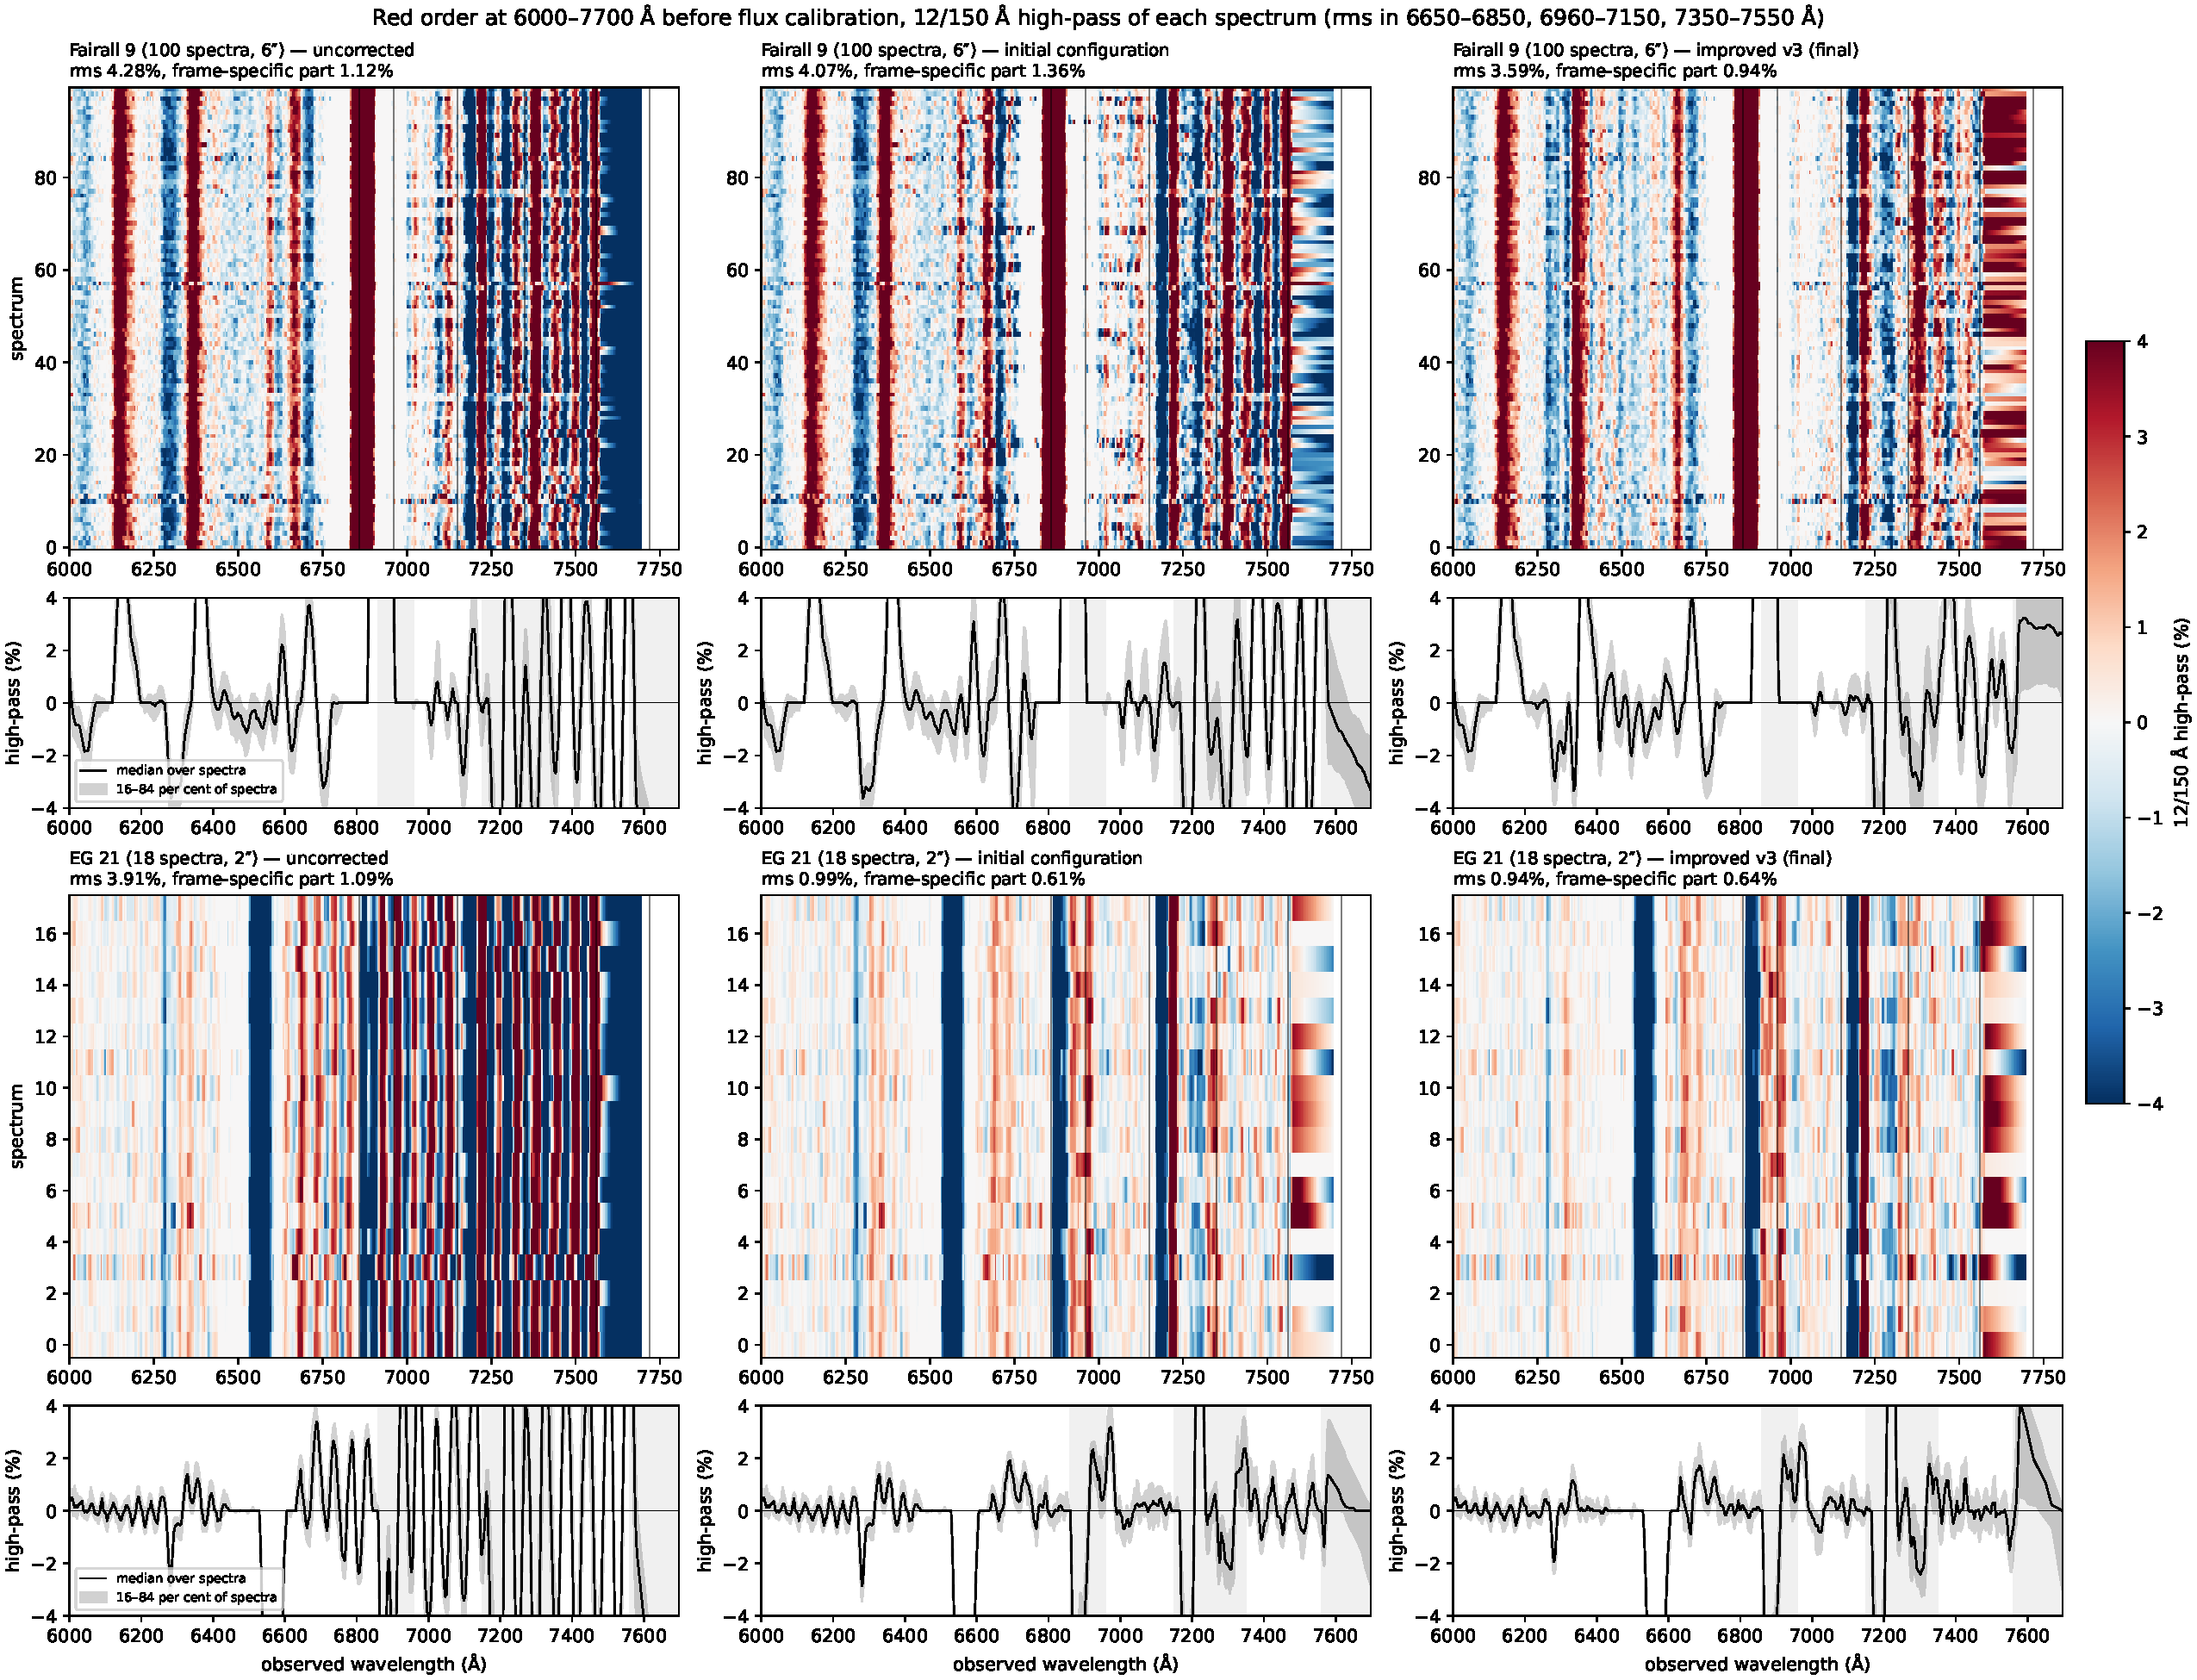
\includegraphics[width=\textwidth]{figures/fig_fringe_band.pdf}
\caption{Small-scale structure of the red order at 6000--7700\,\AA{} before flux calibration: rms of the
12/150\,\AA{} high-pass in the clean windows 6650--6850, 6960--7150 and 7350--7550\,\AA, median over spectra (18 of
EG\,21; all 100 of Fairall~9 in the v3 run, not only the 50 with archive products), for the uncorrected spectra, the
initial configuration of the harmonic fringe model in the pipeline, and improved v3
(Sections~\ref{sec:fringe_pipeline}--\ref{sec:fringe_joint}). For Fairall~9 the frame-specific part (the median over
all spectra removed) separates the fringes from the galaxy's narrow lines ([N\,{\sc ii}], [S\,{\sc ii}]), which the whole high-pass
includes.}
\label{fig:fringe_band}
\end{figure}

\begin{figure}[!htbp]
\centering
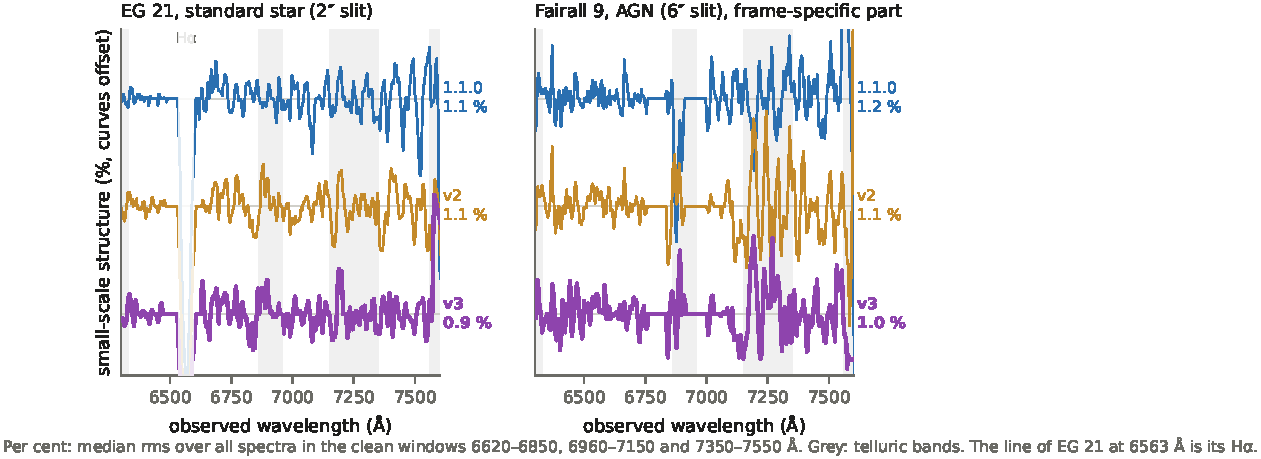
\includegraphics[width=\textwidth]{figures/fig_zoom_6300_7700.pdf}
\caption{Small-scale structure at 6300--7700\,\AA{} (12/150\,\AA{} high-pass of the flux-calibrated red order) in a
typical spectrum (the median rms of improved v3) of EG\,21 (left) and of Fairall~9 (right; the median over spectra
removed, since its narrow lines fall in these windows), for \banzai{}~1.1.0, improved v2 and improved v3, offset for
clarity. Beside each curve: the median rms over all spectra in the clean windows. In this band the three reductions
differ little (1.1 to 0.9 per cent); the fringing that the improved pipeline removes is mostly redward of 7700\,\AA{}
(Fig.~\ref{fig:versions_metrics}). Feige\,110, shown in earlier versions of this figure, is left out: as a flux
standard of these reductions it is flat by construction.}
\label{fig:zoom}
\end{figure}

\begin{figure}[!htbp]
\centering
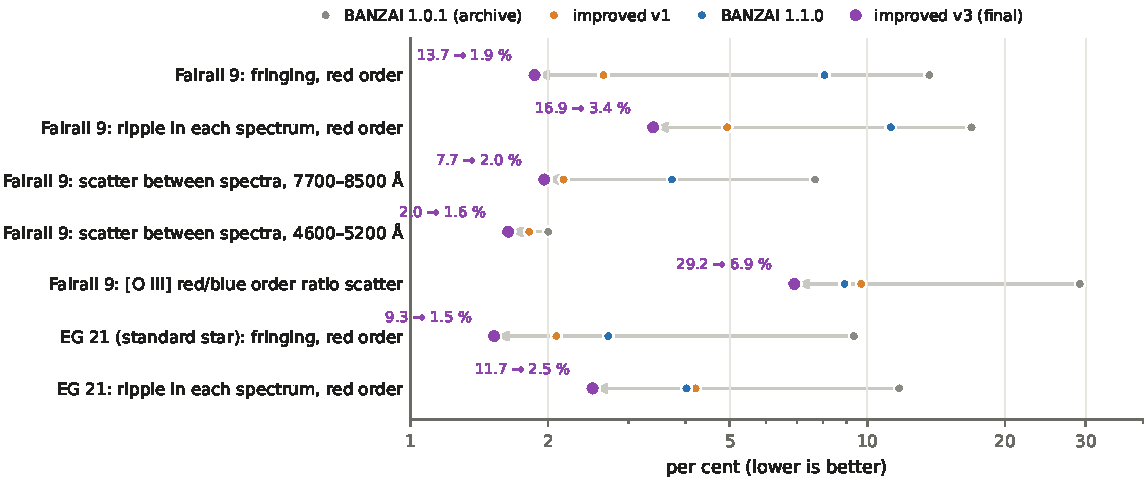
\includegraphics[width=\textwidth]{figures/fig_versions_metrics.pdf}
\caption{Summary of Table~\ref{tab:versions}: each row is one measure of quality (lower is better), each dot a
reduction, and the arrow runs from the archive (\banzai{}~1.0.1) to the final reduction (improved v3), whose values are
written above it. Fringing: the red-order fringe amplitude; ripple: the rms of each spectrum about a power law in the
clean windows of the red order; scatter: the small-scale scatter between the 50 Fairall~9 spectra.}
\label{fig:versions_metrics}
\end{figure}



\section{Uncertainties}
\label{sec:raw_errors}
The uncertainties were tested on the 25 pairs of Fairall~9 exposures taken in the same block (no variability, same
arc, so the bins of the two extractions match one to one). After scaling the second spectrum to the first with a
300\,\AA{} running ratio, the pull $(f_1-f_2)/\sqrt{\sigma_1^2+\sigma_2^2}$ should have unit rms (Fig.~\ref{fig:errors}).
In the 2-d frames the uncertainty is $\sqrt{N+R^2}$ in electrons and the same pixels of the two exposures differ by
1.05\,$\sigma$ on the sky; the extracted error of improved v3 equals the optimal-extraction (Horne) formula
recomputed from the pixels to 1--2 per cent. The extracted pulls are 0.89--0.93 in the blue order and 0.92--1.05 in
the red for improved v3 (1.1.0: up to 1.6 in the red; \banzai{}~1.0.1: 1.7--2.2 beyond 7700\,\AA, where its errors
do not contain the fringe residuals). Measured along the spectrum, which includes exposure-to-exposure differences on
scales of a few pixels, they are 1.09--1.12, rising to 1.2--1.4 in the fringe and telluric regions, and summing 4--30
pixels raises them to $\approx1.2$--1.3: fringe and telluric residuals and small wavelength shifts, which no error
array contains. For integrated line fluxes a systematic term of this size, or the scatter between exposures, should
be added.

\begin{figure}[!htbp]
\centering
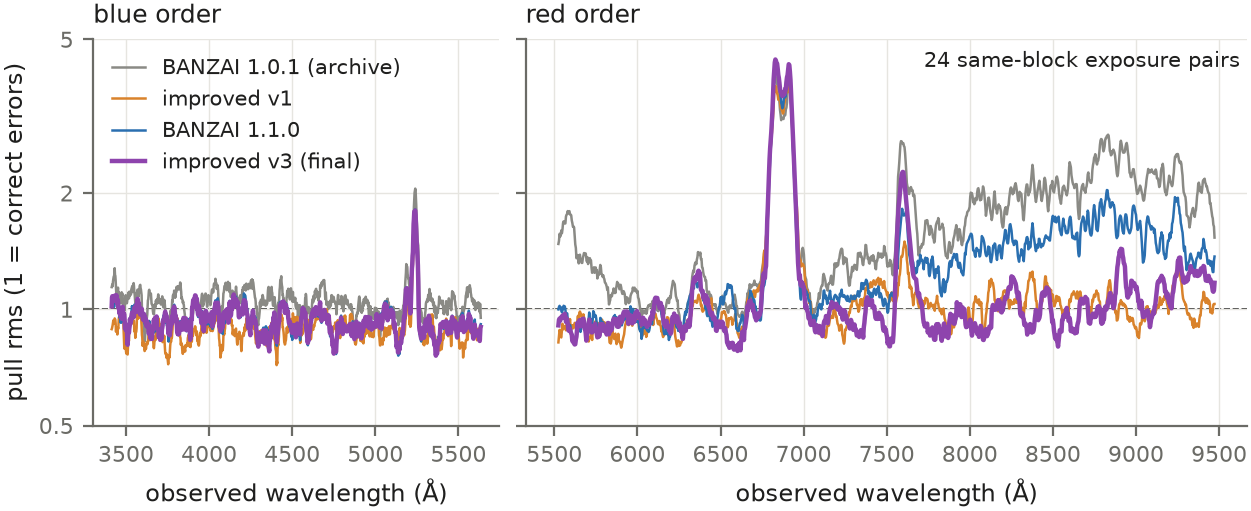
\includegraphics[width=\textwidth]{figures/fig_error_check.png}
\caption{Robust rms of the pull of 25 same-block Fairall~9 exposure pairs, per wavelength (smoothed); 1 means
correct uncertainties. Blue order left, red order right.}
\label{fig:errors}
\end{figure}


\chapter{The final pipeline (improved v3) at both FLOYDS sites}
\label{sec:sites}

Improved v3 is our final version of the pipeline for now. This chapter lists what it contains, describes the three
additions made after the first v3 run (arc lines in the arc fit, a trace template per site, two more flux
standards), applies it to a second data set from the other FLOYDS (Faulkes Telescope North, Haleakal\=a; site code
OGG), and verifies every step at both sites with the same measurements. Both data sets were reduced from raw with the
final code in one pass each (\texttt{banzai\_floyds\_offline}; COJ: 412 frames, OGG: 421 frames, no failures).

\section{What the final version contains}
\label{sec:sites_final}
\begin{itemize}
\item \textit{Order trace}: order shape from the sky flats of \texttt{data/orders/skyflats.dat}; the per-frame shift as
in \banzai{}~1.1.0. Sky flats already processed by the LCO archive (\texttt{-f91} files) are accepted as they are.
\item \textit{Arcs}: the \banzai{}~1.1.0 2-d arc fit with five more lines (Hg\,4916 in both orders, Ar\,6416, 6677,
6753 and 6767 in the red; Section~\ref{sec:sites_arcs}).
\item \textit{Object trace}: the physical model of eq.~(\ref{eq:tracehybrid}) with a template and priors for each site
(Section~\ref{sec:sites_trace}).
\item \textit{Object wavelength zero point}: from the telluric bands in the object's own light, transferred to the
blue order (Section~\ref{sec:wl_zp}).
\item \textit{Fringes}: no 2-d division; the harmonic model with the phase from a lamp-flat phase master, fitted jointly
with a telluric template, plus a residual template per slit (Sections~\ref{sec:fringe_pipeline}--\ref{sec:fringe_joint}).
\item \textit{Telluric}: transmission applied only inside the absorption bands, median of the nine nearest standards;
the O$_2$ A band flagged in science spectra (Section~\ref{sec:flux_tell}).
\item \textit{Flux}: ensemble of the nine nearest standards with the grey level from the clearest half
(Section~\ref{sec:flux_ensemble}); Feige\,67 and GD\,153 added to the standards (Section~\ref{sec:sites_flux}).
\end{itemize}
Every frame records what was applied in its header (\texttt{L1TRCMOD}, \texttt{L1TRCADR}, \texttt{L1WZP1/2},
\texttt{L1FRGMET}, \texttt{L1FRGJNT}, \texttt{L1FRGTPL}, \texttt{L1TELNST}, \texttt{L1TELFLG}, \texttt{L1FLXNST},
\texttt{L1FLXGRY}). All 176 unit tests of the package pass.

\section{The OGG data set}
\label{sec:sites_data}
The OGG set (Table~\ref{tab:oggdata}) is an RM campaign on NGC\,4151 through the 6\,arcsec slit, with BD$+28^\circ4211$,
GD\,153 and Feige\,67 through the 2\,arcsec slit, from 2024 November 20 to 2025 August 30. Every science and standard
exposure has its arc and lamp flat. The only sky flats in \texttt{skyflats.dat} for OGG are from 2019 March 29; they
were used as processed by the archive. NGC\,4151 ($z=0.003326$) is bright and has very strong narrow lines, so it
tests the wavelength scale and the flux calibration well; its broad H$\alpha$ and [S\,{\sc ii}] vary and fall in two of
the three 6500--7500\,\AA{} windows used for Fairall~9, so for NGC\,4151 only the line-free window 6960--7150\,\AA{} and
the differences between the two exposures of a visit measure the fringe residual.

\begin{table}[!htbp]
\centering
\caption{The OGG data set (\texttt{ogg2m001-en06}, FLOYDS on the Faulkes Telescope North).}
\label{tab:oggdata}
\begin{tabular}{lccc}
\toprule
Frames & Slit & $N$ & Dates \\
\midrule
NGC\,4151, 300\,s & 6\,arcsec & 60 (30 visits) & 2024 Nov 20 -- 2025 Jul 21 \\
BD$+28^\circ4211$ & 2\,arcsec & 68 & 2025 Jun 7 -- Aug 30 \\
GD\,153 & 2\,arcsec & 20 & 2025 May 2 -- Jun 1 \\
Feige\,67 & 2\,arcsec & 12 & 2025 Mar 24 -- Apr 7 \\
Arcs / lamp flats & 6 and 2\,arcsec & 130 / 131 & \\
Sky flats (2019 Mar 29, archive-processed) & 1.2, 1.6, 2, 6\,arcsec & 4 & \\
\bottomrule
\end{tabular}
\end{table}

\section{Arc lines added to the arc fit}
\label{sec:sites_arcs}
Chapter~\ref{sec:wavelength} found that Hg\,4916 and Ar\,6416, 6677 and 6753/6767 are detected in the arcs but not used,
leaving H$\beta$--[O\,{\sc iii}] and H$\alpha$ to interpolation; in improved v1 they were used to correct the archive
products afterwards (Section~\ref{sec:wl_refit}). In the final version they are part of the arc fit itself: they are
in the list of used lines of \texttt{arc\_lines.py}, with strengths relative to Hg\,5461 measured on 158 arcs through
the 2\,arcsec and narrower slits of both sites (Hg\,4916: 0.0029; Ar\,6416: 0.0038; 6677: 0.0054; 6753: 0.0037; 6767:
0.0002). They are faint (0.2--0.5 per cent of Hg\,5461), so the arc fit treats them with a fixed line profile like
the other faint and blended lines.

The \banzai{}~1.1.0 arc fit is already much better than the 1.0.1 solution of the archive: measured with the group
model of eq.~(\ref{eq:arcgroup}) on each arc's own wavelength map, the 1.1.0 solution is off at the unused lines by
at most 0.6\,\AA{} (COJ; $-8$\,\AA{} in 1.0.1) and 0.2\,\AA{} (OGG). Adding the lines removes most of what is left
where it matters for RM (Fig.~\ref{fig:arc_lines}): at COJ the red-order error at Hg\,4916 goes from $+0.59$ to
$-0.06$\,\AA{} and the difference between the two orders there from 1.07 to 0.32\,\AA; the lines already used do not
move ($<0.1$\,\AA). The added lines enter the fit in 41 (Hg\,4916) to 99 per cent (Ar\,6677) of the COJ arcs. At OGG
they are fainter, enter the fit in at most 41 per cent of the arcs (Hg\,4916 in none), and change nothing, since the solution was already
right there. On the science, the red--blue [O\,{\sc iii}] difference of Fairall~9 goes from $+0.61\pm0.79$ to
$+0.30\pm0.79$\,\AA.

\begin{figure}[!htbp]
\centering
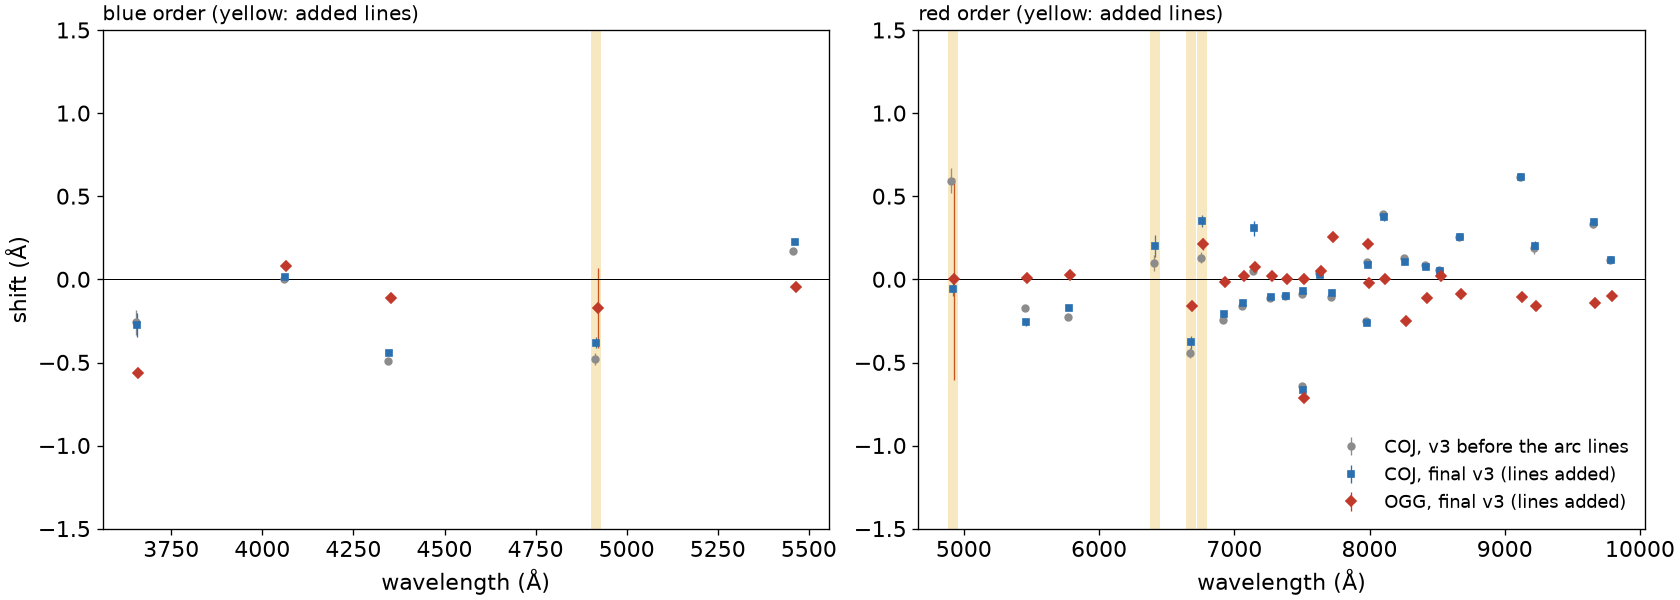
\includegraphics[width=\textwidth]{figures/fig_arc_lines.png}
\caption{Median shift of every arc line group on the arcs' own wavelength solutions (eq.~\ref{eq:arcgroup}), blue
order left and red right: COJ before (grey) and after (blue) adding the lines to the arc fit, and OGG with the lines
(red). Yellow: the added lines. Error bars: scatter over the arcs divided by $\sqrt{N}$.}
\label{fig:arc_lines}
\end{figure}

\section{A trace template for each site}
\label{sec:sites_trace}
The instrumental shape $S_o(\lambda)$ of the object-trace model (eq.~\ref{eq:tracemodel}) belongs to the instrument,
so OGG needs its own. It was built, as for COJ, from the chunk centroids of all OGG standards (100 frames; script
\texttt{build\_trace\_template.py}); it spans $-0.28$ to $+0.45$\,px (red) and $-0.17$ to $+0.21$\,px (blue), and the
smoothed template follows the stacked median to 0.014 and 0.012\,px. The priors are $c_1-c_2=-0.18\pm0.18$\,px and
$a=0.24\pm0.51$ (COJ: $-0.87\pm0.29$ and $0.58\pm0.14$). The fitted refraction scale varies much more from frame to
frame at OGG (the standards range from $\approx-0.1$ to 0.3, NGC\,4151 has $0.89\pm0.21$), so its prior is broad and
each frame's own centroids decide. Without a template the pipeline falls back to the 1.1.0 polynomial; with it, every
OGG frame uses the physical model (\texttt{L1TRCMOD = 'adr'}).

\section{Flux standards and a throughput step at OGG}
\label{sec:sites_flux}
In a first OGG reduction only BD$+28^\circ4211$ was a flux standard: GD\,153 and Feige\,67 are not in the \banzai{}
catalogue. NGC\,4151's [O\,{\sc iii}] flux, which should be constant, then scattered by 26 per cent, because of a
step: $6.8\times10^{-12}$ until 2025 March 28 and $1.2\times10^{-11}$\,erg\,s$^{-1}$\,cm$^{-2}$ from May 10, a factor of
1.8 in both orders. The step is real light: the raw counts and the sum over the whole order in 2-d show the same
factor, the extraction window holds 92--96 per cent of the light throughout, and the lamp flats and arcs (which do
not use the telescope) stay constant to 10 per cent. It is therefore a change of the telescope throughput between
2025 April 7 and May 2 (the last Feige\,67 and the first GD\,153 exposure): Feige\,67 in March--April comes out at
about half its catalogue flux, GD\,153 in May at its catalogue flux. All BD$+28^\circ4211$ standards are from after the
step (June--August), so every frame before it was calibrated $\approx1.8$ times too faint.

The fix is a standard before the step. Feige\,67 (Oke 1990, 3200--9200\,\AA; ESO \texttt{okestan}) and GD\,153 (ESO
X-shooter library) were added to \texttt{data/standards} in the format of the other references, at the positions LCO
observes them (GD\,153 is $5''$ from its J2000 position because of its proper motion). The Feige\,67 reference ends at
9200\,\AA, and the flux code holds a reference constant beyond its end, which would corrupt the red end of the
sensitivity; it is extended to 11\,000\,\AA{} with a power law fitted to its own 7500--9200\,\AA{} continuum (index
$-3.99$, the Rayleigh--Jeans slope of this hot subdwarf; header keywords \texttt{EXTRAP}, \texttt{EXTRAPSL}). With
the two standards, the NGC\,4151 [O\,{\sc iii}] flux scatters by 9.4 per cent (COJ Fairall~9: 12.5 per cent over all
100 spectra) and the levels before and after the step agree to 7 per cent (Fig.~\ref{fig:sites}); the remaining 7 per
cent is plausibly the older Feige\,67 reference against the HST-based ones. The scatter that remains at both sites
is mostly clouds and slit losses during the science exposures themselves (single exposures at 0.7 and 1.3 times the
median have low counts or high airmass), which no calibration can remove and which the RM scaling to
[O\,{\sc iii}] is designed for; the red/blue ratio, which they do not affect, scatters by 6--6.5 per cent. The 8 NGC\,4151 spectra of 2024 November and
December have no standard within 90\,d; they use the nearest one (Feige\,67, before the step) instead of an ensemble.

Two lessons follow. The ensemble of the nearest standards is only valid if the throughput does not change within it;
the nine nearest standards of a frame close to a step would mix both sides (here no NGC\,4151 frame falls between
April 7 and May 2, so this did not happen). And a campaign needs standards throughout, of a star in the catalogue
(Chapter~\ref{sec:recommendations}).

\section{The object zero point on NGC\,4151}
\label{sec:sites_zp}
NGC\,4151 is a strong test of the telluric zero point (Section~\ref{sec:wl_zp}): its zero points range from $-10$ to
$+17$\,\AA{} in the red order (median $+10.7$\,\AA), i.e.\ the nucleus sits up to $\approx\pm2''$ from the slit centre
from visit to visit. Before the correction the [O\,{\sc iii}] position scatters by 6.2\,\AA{} (red) and 3.1\,\AA{}
(blue); after it by 0.94 and 0.53\,\AA. Fairall~9 at COJ behaves the same way: without the correction its
[O\,{\sc iii}] position scatters by 6.5\,\AA{} (red) and 3.2\,\AA{} (blue) in the final reduction, with it by 0.69
and 0.45\,\AA{} (Fig.~\ref{fig:sites}). For both targets the correction is what aligns the epochs. Without this step the NGC\,4151
spectra would be misaligned by up to 27\,\AA{} between epochs.

\section{Verification of every step at both sites}
\label{sec:sites_verify}
Table~\ref{tab:sites} and Fig.~\ref{fig:sites} collect the measurements of every step, made with the same script on
both sites (\texttt{v3\_verify.py}). COJ is shown before and after the arc lines were added; the other COJ numbers
do not change. All 317 spectra use the physical trace model, the joint fringe and telluric fit, and (science frames)
the nine-standard telluric and flux ensembles.

\begin{table}[!htbp]
\centering
\caption{Verification of the final pipeline. Science: Fairall~9 at COJ (100 spectra), NGC\,4151 at OGG (60). Wavelengths
in \AA; residuals and scatters in per cent; pulls are the robust rms of $(f_1-f_2)/\sigma$ for the two exposures of
each visit (1 = correct uncertainties). Standards: rms of flux over reference in the clean windows (6500--7500\,\AA)
and at 7750--8900\,\AA.}
\label{tab:sites}
\small
\begin{tabular}{llccc}
\toprule
Step & Measurement & COJ, v3 before & COJ, final & OGG, final \\
 & & arc lines & v3 & v3 \\
\midrule
Arcs & median error of the used lines, rms (\AA) & 0.49 & 0.49 & 0.15 \\
 & largest median error at the added lines (\AA) & 0.59 & 0.38 & 1.3$^{a}$ \\
Trace & frames with the physical model (\%) & 100 & 100 & 100 \\
Zero point & science: [O\,{\sc iii}] scatter, red / blue (\AA) & 0.62 / 0.48 & 0.69 / 0.45 & 0.94 / 0.53 \\
 & science: [O\,{\sc iii}] red $-$ blue (\AA) & $+0.61\pm0.79$ & $+0.30\pm0.79$ & $+1.39\pm0.88$ \\
Fringes & science: red fringe metric (\%) & 2.01 & 1.95 & 2.51 \\
 & science: clean window 6960--7150\,\AA{} (\%) & 0.58 & 0.58 & 0.86 \\
 & science: same-visit difference, 6500--7500\,\AA{} (\%) & 0.65 & 0.66 & 0.69 \\
Telluric & science: water band 7170--7330\,\AA{} (\%) & 1.91 & 1.92 & 2.19 \\
 & science: water band 8130--8360\,\AA{} (\%) & 3.35 & 3.21 & 2.70 \\
Flux & science: [O\,{\sc iii}] flux scatter, blue / red (\%) & 12.6 / 13.3 & 12.5 / 14.0 & 9.4 / 12.5 \\
 & science: red/blue [O\,{\sc iii}] ratio scatter (\%) & 6.1 & 6.5 & 6.2 \\
 & standard over reference, 6500--7500 / 7750--8900\,\AA{} (\%) & 0.93 / 1.92 & 0.97 / 2.00 & 0.71 / 1.12$^{b}$ \\
 & independent star: EG\,21 shape, 6500--7500\,\AA{} (\%) & 1.13 & 1.09 & -- \\
Errors & science: pull, blue order (no unit) & 0.95--1.05 & 0.95--1.06 & 0.90--1.01 \\
 & science: pull, red order (no unit) & 0.93--1.07 & 0.94--1.06 & 0.98--1.27 \\
\bottomrule
\end{tabular}
\par\smallskip\raggedright\footnotesize
$^{a}$Ar\,6416, detected in only 3 OGG arcs. $^{b}$BD$+28^\circ4211$ (GD\,153: 1.16 / 2.23; Feige\,67: 0.90 / 1.47);
COJ: Feige\,110.
\end{table}

\begin{figure}[!htbp]
\centering
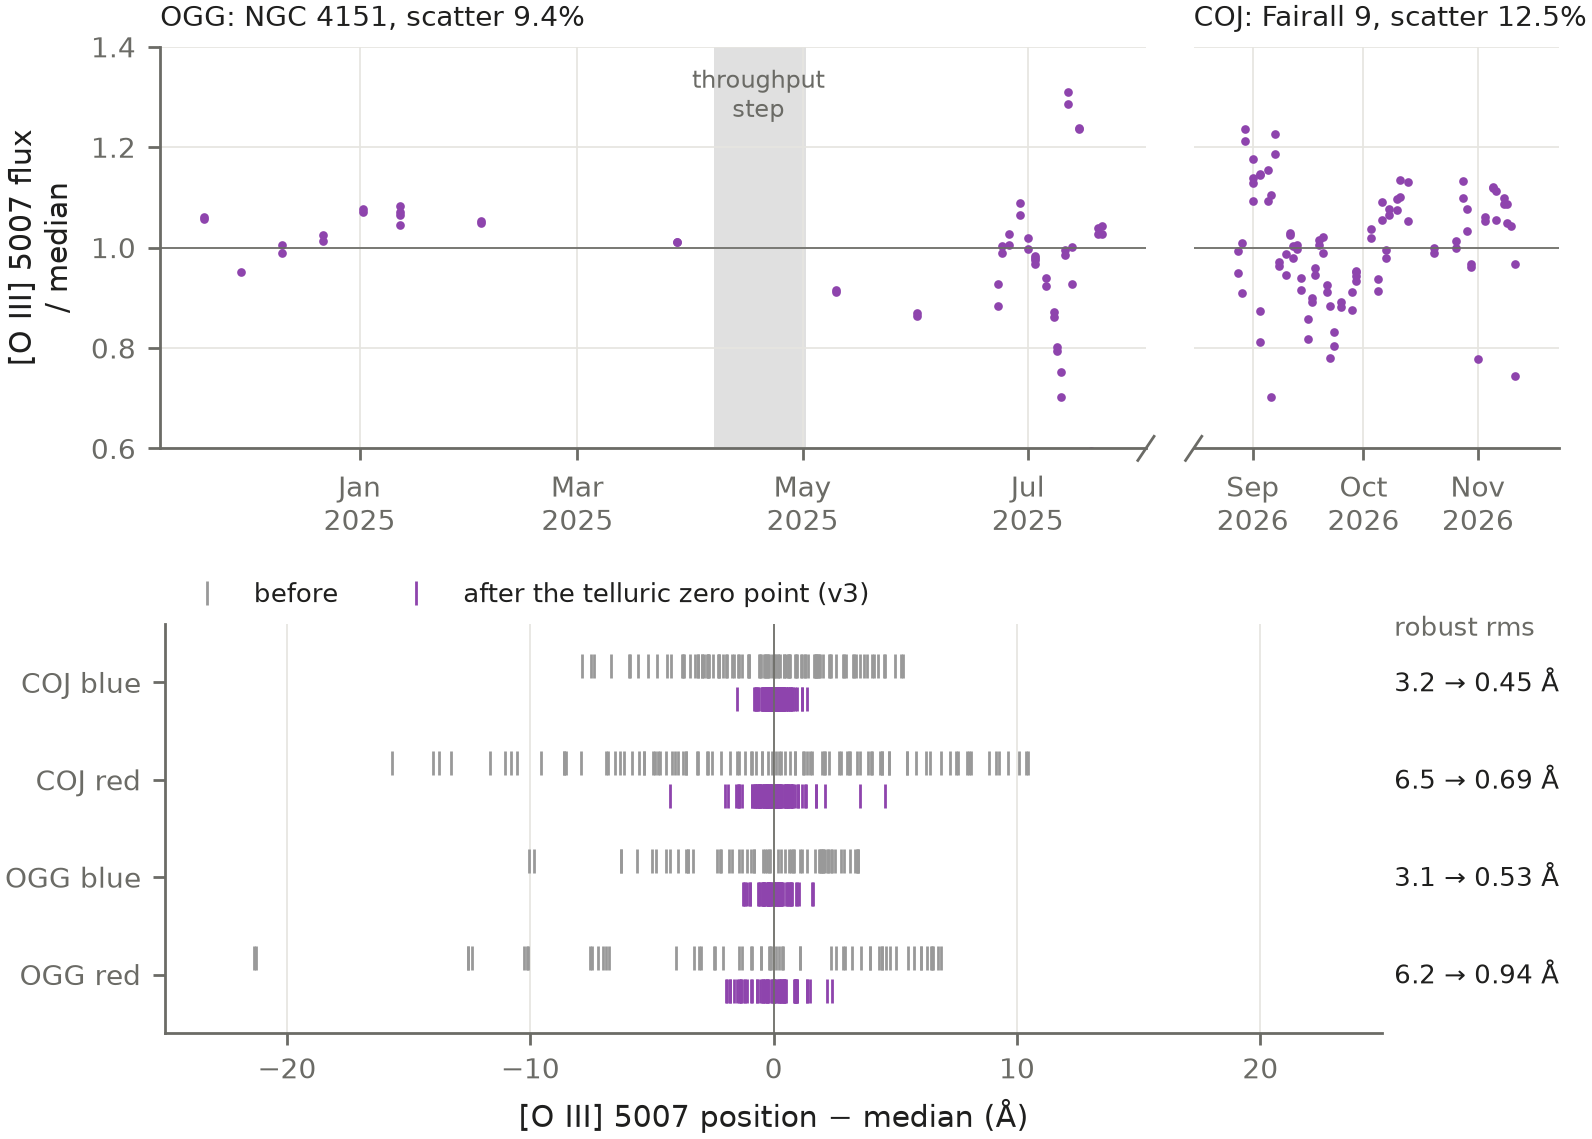
\includegraphics[width=\textwidth]{figures/fig_sites.png}
\caption{The final pipeline at both sites. Top left: [O\,{\sc iii}]\,5007 flux of every exposure (blue order) over
its median; grey band: the OGG throughput step, bridged by the added standards. Top right: pull rms of the two
exposures of each visit (1 = correct uncertainties). Bottom left: [O\,{\sc iii}] position of every exposure before
(grey) and after (colour) the telluric zero point. Bottom right: median flux standard over its reference at
fringe scales (Feige\,110 at COJ, BD$+28^\circ4211$ at OGG; the telluric bands are flat by construction).}
\label{fig:sites}
\end{figure}

\textit{Reading the comparison.} The two sites agree to within what their targets allow. The OGG pull rises to 1.2--1.3
redward of 6500\,\AA: NGC\,4151 has a 2.4 times higher signal-to-noise ratio per bin than Fairall~9, so the same fringe and telluric
residuals, which are not in the error array (Section~\ref{sec:raw_errors}), weigh more against the photon noise. The
red fringe metric of NGC\,4151 (2.5 per cent) includes its own O\,{\sc i}\,8446 and Ca\,{\sc ii}/Paschen lines in the windows; the
difference between the two exposures of a visit, which removes everything static, is the same at both sites
(0.66--0.69 per cent). The red--blue [O\,{\sc iii}] difference at OGG (1.4\,\AA) is larger than at COJ (0.3\,\AA)
because the added arc lines rarely enter the OGG fit; it is a constant per site and is removed by the usual alignment
on [O\,{\sc iii}].

\section{Disk space}
\label{sec:sites_disk}
A processed 2-d spectrum is 47\,MB, of which 43\,MB is the uncompressed \texttt{BINNED2D} table. None of the 2-d
diagnostic content is read back by the pipeline, so after a run the finished 2-d spectra are made lean
(\texttt{lean\_2d.py}: the \texttt{PROFILE}, \texttt{BACKGROUND} and \texttt{FRINGE} images are dropped, and
\texttt{BINNED2D} is kept only in a few example frames), and the arcs and lamp flats lose their \texttt{BINNED2D}
during the run. A site-season of $\approx$400 frames then takes $\approx2$\,GB, of which 1.2\,GB are the processed
calibrations kept for re-reducing the science; the \texttt{-1d} spectra are 0.6\,MB each.

\chapter{Cosmic rays, the sky model and quality flags}
\label{sec:cosmics}

This chapter comes from a search for the worst reductions of the final pipeline (improved v3). The two worst kinds of
frame were not caused by the steps of the earlier chapters but by two parts of \banzai{} we had not examined: the
cosmic-ray detector (LA Cosmic) and the sky model under the object. In both, the extracted spectrum scatters far more
than its errors. The cosmic-ray detector also clips the peaks of bright emission lines; in one NGC\,4151 frame this
made H$\alpha$ 2.6 times too bright. A cosmic-ray detector can always be tuned to look good on the cases it was tuned
on, so most of the chapter is about testing the changes on data they were not tuned on. The changes are in the code
(branch \texttt{rm-improvements} of \banzai{}), but \textbf{the products of this report have not been re-reduced with
them}; Table~\ref{tab:cr_status} gives the status of each change.

\paragraph{Summary of the chapter.} For each problem: what went wrong, what we changed, how we tested it, and the result.
\begin{itemize}
\item \textit{Bright star cores and emission-line peaks taken for cosmic rays}
(Sections~\ref{sec:cr_method}--\ref{sec:cr_lines}). LA Cosmic in \banzai{}~1.1.0 flags the cores of bright stars and
the peaks of narrow emission lines, and it misses real cosmic rays that land on these bright regions.
\textit{Change} (Section~\ref{sec:cr_model}): before LA Cosmic searches the frame, we subtract a smooth model of the
object (a 7-pixel running median along each detector row), so that only features sharper than the object are left.
\textit{Tests} (Section~\ref{sec:cr_verify}): artificial cosmic rays added to real frames, and a comparison of the two
exposures of each visit for 106 frames. \textit{Result}: in the brightest standard star the flagged share of the core
falls from 46 to 0.1 per cent; on the worst H$\alpha$ line the flagged pixels fall from 179 to 15 and its flux from
2.64 to 1.02 times that of the other exposure; of the artificial cosmic rays above 10$\sigma$ on line peaks and star
cores, 97 instead of 66 per cent are found. The cost is a few more small false detections per frame on the trace of
bright objects (median 1 to 5 per frame at OGG), which do not change the extracted fluxes beyond the noise.
\item \textit{Line peaks that the object model still flags} (Section~\ref{sec:cr_pair}). \textit{Change}: a new
pipeline stage, the \textit{same-visit check}, compares each exposure after LA Cosmic with the other exposure of its
visit and removes flags on features that are present in both. \textit{Tests}: artificial cosmic rays in 8 frames, and
the whole sample of 106 frames. \textit{Result}: it finds the same artificial cosmic rays as the object model alone and
flags 22 (OGG) and 10 (COJ) per cent fewer pixels. It removes the 15 pixels still flagged on the worst H$\alpha$, and
it brings the flagged pixels on the narrow lines of NGC\,4151 to 215, against 236 with \banzai{}~1.1.0 and 398 with
the object model alone.
\item \textit{The sky model beside a wide object} (Section~\ref{sec:cr_sky}). When a wide object leaves little sky in
the slit, the sky model follows the noise and the spectrum scatters 3--4 times its errors. \textit{Change}: a sky line
must also stand out from the scatter of the first-pass sky by 5 robust standard deviations. \textit{Result}: in the affected frames the
scatter falls from 3.0--3.3 to 1.1--1.2 times the errors; in normal frames the flux changes by less than 0.2 per cent.
\item \textit{A guard in the extraction} (Section~\ref{sec:cr_guard}). A wavelength bin that has lost more than half
of its profile weight to cosmic-ray flags is now masked instead of being scaled up from the rest.
\item \textit{Quality keywords} (Section~\ref{sec:qc}). Every product now carries per-frame quality measures and flags
in its header. They were added to all 317 science and standard products of improved v3, and they find the problem
frames that we found by hand in this report.
\end{itemize}

\section{How \banzai{} finds cosmic rays}
\label{sec:cr_method}
\banzai{}~1.1.0 runs LA Cosmic \citep{vanDokkum2001}, as implemented in the Python package \texttt{astroscrappy}, on
each science and standard frame. The names in typewriter font below are the parameters of LA Cosmic. Step by step:
\begin{enumerate}
\item \textit{Sky.} A first sky model $B(x,y)$ is fitted outside a mask around the object trace: a spline in wavelength
times a low-order polynomial along the slit.
\item \textit{Inputs.} LA Cosmic receives the frame $D$ in electrons, its variance from the pipeline's error map, and
$B$ as the background to subtract. It also receives a mask of pixels it must not search: bad pixels, pixels outside the
orders, and a band 2 pixels wide along the edges of each order, because those edges are sharp.
\item \textit{Sharpness.} LA Cosmic subtracts the background, takes the Laplacian of the frame sampled at twice the
resolution, and divides it by the noise: $S=\nabla^2(D-B)/2\sigma$, where $\sigma$ is the noise of the pixel. It then
subtracts the 5-pixel median of $S$ from $S$, to remove its smooth part. A cosmic ray deposits its charge in one or a
few pixels and is far sharper than anything the optics produce, so its $S$ is large.
\item \textit{Candidates.} Pixels with $S>5$ (\texttt{sigclip}) are candidates.
\item \textit{Fine-structure test.} A star or a line is also sharp, but it is as wide as the seeing. LA Cosmic
therefore builds a fine-structure image $F$: the 3-pixel median of the frame minus the 7-pixel median of that. It keeps
a candidate only if its Laplacian is more than 5 times $F$ (\texttt{objlim}).
\item \textit{Growth.} The neighbours of a detected pixel are added to it if their $S$ exceeds
$\texttt{sigfrac}\times\texttt{sigclip}$. \banzai{} uses $\texttt{sigfrac}=0.03$, i.e.\ a threshold of 0.15$\sigma$,
ten times below the LA Cosmic default (0.3). As a result a detection grows over the whole of any bright region it
touches. The detected pixels are replaced by the mean of their unmasked neighbours, and steps 3--6 are repeated four
times.
\item \textit{Fill.} Holes inside a detection are filled in, and its pixels are marked with bit 8 of the mask.
\item \textit{Use.} The sky is fitted again without the flagged pixels, and the extraction leaves them out. In each
wavelength bin the flux is $f=\sum a(d-b)/\sum aP$ over the remaining pixels, where $d$ is the value of a pixel, $b$
the sky model there, $P$ the spatial profile model of the object and $a$ the weight of the pixel in the extraction.
A flagged pixel therefore loses no flux \textit{if the profile model $P$ is right}.
\end{enumerate}

\textit{Which versions do this.} \banzai{}~1.0.1, which made the archive products, has no cosmic-ray detection at all.
The detector of improved v3 is that of \banzai{}~1.1.0 unchanged: the code, its parameters, its place in the order of
pipeline stages and the sky fit before it are identical to the 1.1.0 release. Only its input differs, in two ways.
First, 1.1.0 divides the 2-d frame by the lamp-flat fringe pattern before the detector runs, and improved v3 does not
(Chapter~\ref{sec:fringe}). Second, in improved v3 the object trace that sets the sky mask comes from the physical
trace model (Chapter~\ref{sec:traces}). Neither changes the flags. We checked this on the 46 Fairall~9 frames of the
test of Section~\ref{sec:cr_verify}: \banzai{}~1.1.0 as released (without the object wavelength zero point) and
improved v3 have the same number of real and false detections on the object (136 and 134 real, 1414 and 1420 false),
in the same frames. The problems of this chapter are therefore those of \banzai{}~1.1.0. There is no reduction of OGG
with 1.1.0 as released; since the code is the same, we expect the same star cores and H$\alpha$ to be flagged there.

\section{The core of a bright star taken for cosmic rays}
\label{sec:cr_stars}
The brightest standard star is BD$+28^\circ4211$ at OGG, with peaks of 30\,000--45\,000\,e$^-$ per pixel through the
2\,arcsec slit. In good seeing LA Cosmic flags the core of the star. We measured the share of the trace core (the
pixels within one FWHM of the trace) that is flagged. It is more than 1 per cent in 10 of the 68 spectra of this star
and more than 5 per cent in 6 of them. On 2025 August 19 (seeing 1.3\,arcsec) it is 46 per cent of the core in the blue
order (Fig.~\ref{fig:cr_smoothing}, top). The extraction then works from the wings of the profile, where the profile
model is least right, and the spectrum scatters 2.9 times its errors from bin to bin. No other standard and no AGN frame
is affected: Feige\,110 and the other standards are fainter, and an AGN through a 6\,arcsec slit has a broader profile.
That is why the problem appeared only among the OGG standards.

\section{Emission lines taken for cosmic rays}
\label{sec:cr_lines}
A bright narrow emission line is sharp along the dispersion. In all 160 AGN spectra of improved v3 we looked for flags
on the trace core within $\pm12$\,\AA{} of [O\,{\sc iii}]\,$\lambda\lambda$4959, 5007, H$\beta$ and
H$\alpha$+[N\,{\sc ii}]:
\begin{itemize}
\item \textit{[O\,{\sc iii}]\,5007} is never flagged, in either object.
\item \textit{[O\,{\sc iii}]\,4959.} In one Fairall~9 frame (2026 August 28) five pixels of the core of the line are
flagged. They are false positives, because they agree with the other exposure of the visit within the noise; they have no
measurable effect on the flux.
\item \textit{[O\,{\sc iii}]\,4959 in 12 NGC\,4151 frames.} These flags are a warm detector pixel of the OGG camera at
$(x,y)=(1465,409)$, with 24\,500\,e$^-$ against 500--1000 in its neighbours. It is not in the bad-pixel mask, and it
falls on the wing of the line because NGC\,4151 is always placed at the same position in the slit. Masking it is right.
\item \textit{H$\alpha$ of NGC\,4151} is flagged in 7 of 60 frames, by up to 179 pixels covering the peak of the line
(Fig.~\ref{fig:cr_halpha}). The two exposures of a visit normally agree on the H$\alpha$+[N\,{\sc ii}] flux to 2.5 per
cent. Two exposures with clipped lines had 2.64 and 1.18 times the flux of the other exposure of their visit. In the
other five the flags changed the flux by no more than the noise (one pair differs by 6 per cent with or without flags).
\end{itemize}
The flux is biased upwards, and the bias can be large, because of how the extraction treats flagged pixels
(Section~\ref{sec:cr_method}, step 8). With the core of the line removed, what is left in the bin is the wings of an
emission region that is resolved along the slit (the narrow-line region of NGC\,4151 is extended). Their flux is divided
by the small profile weight of those wings, as if they held the same fraction of the light as in the continuum.
\textit{This can happen in any bright object with strong narrow lines in good seeing}---Seyfert galaxies, H\,{\sc ii}
galaxies, planetary nebulae. It is not visible in the extracted spectrum unless one compares exposures: the spectrum
simply shows an H$\alpha$ that is too strong.

\begin{figure}[!htbp]
\centering
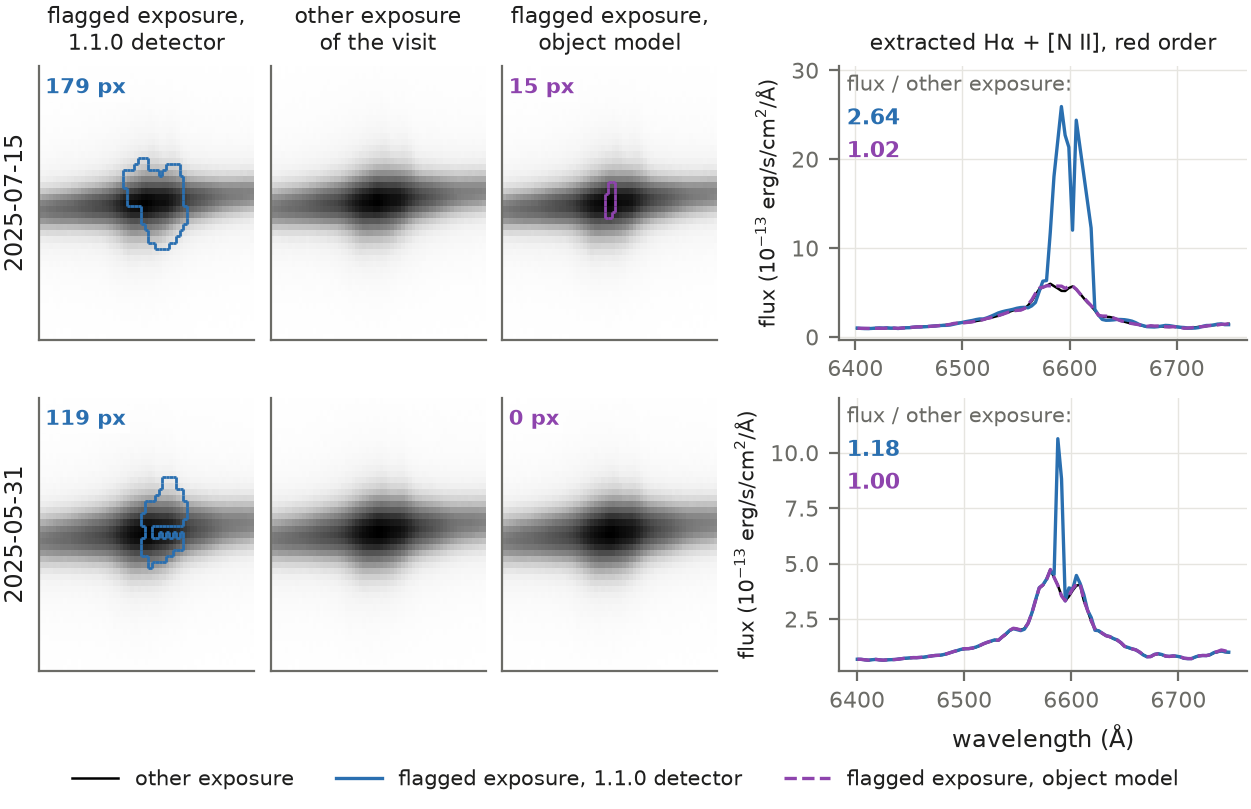
\includegraphics[width=\textwidth]{figures/fig_cr_halpha.png}
\caption{H$\alpha$ of NGC\,4151 flagged as cosmic rays (OGG, 6\,arcsec slit). Left: the 2-d frame around H$\alpha$
(counts, same arcsinh grey scale in a row) of the flagged exposure with the flags of the 1.1.0 detector of improved v3
(blue), the other exposure of the same visit, and the flagged exposure with the object model (purple). Right: the
extracted H$\alpha$, with the H$\alpha$+[N\,{\sc ii}] flux of the flagged exposure divided by that of the other
exposure. Top: 2025 July 15, 179 pixels flagged and the flux 2.64 times too high; with the object model 15 pixels are
flagged, the four bins where they remove most of the profile are masked by the extraction guard
(Section~\ref{sec:cr_guard}) and the ratio is 1.02. Bottom: 2025 May 31, 119 pixels and 1.18; with the object model
none and 1.00.}
\label{fig:cr_halpha}
\end{figure}

\section{A related problem: the sky model beside a wide object}
\label{sec:cr_sky}
\textit{The problem.} The worst Fairall~9 spectra (six frames on 2026 September 3, 6 and 16) scatter 3--4 times their
errors from bin to bin, although their 2-d frames have the noise their error maps predict. The excess is already in the
extraction before any correction, in both the optimal and the unweighted sums, and it is absent from a plain box
sum of the same pixels. It therefore comes from the sky model.

\textit{The cause.} The sky model is a spline in wavelength, with knots one pixel apart on sky lines and three pixels
apart elsewhere. Sky lines are found as the pixels of a first-pass sky model that are more than 15 per cent above its
running median. In these frames the Moon was up (58--80 per cent illuminated) and the seeing was 2.6--4.5\,arcsec, so
Fairall~9 fills much of the slit. The mask that keeps the object out of the sky fit is then narrowed to less than
6 times the width ($\sigma$) of the spatial profile on each side (header keyword \texttt{L1BKMW}\,$<6$), and few sky
pixels are left. The first-pass sky is noisy, its noise passes the 15 per cent test, and nearly every column gets a
knot (1464 instead of $\approx500$). The sky under the object then follows the noise of a few pixels at the edges of
the slit, multiplied by the number of pixels in the extraction window. Two measurements show this. The bin-to-bin
second differences of the extracted flux and of the sky are anticorrelated, with coefficients of $-0.95$ to $-0.97$.
And the sky model scatters by 3.5--3.8 times the flux errors, against 0.1 in normal frames. The same noisy sky also
makes LA Cosmic flag the object: the two frames of 2026 September 3 each have $\approx$240 flagged groups on the object
that are not in the other exposure (Section~\ref{sec:cr_verify}).

\textit{The change.} A sky line must now also stand out from the scatter of the first-pass sky by 5 robust standard
deviations. \textit{Result}: on the affected frames the scatter falls from 3.0--3.3 to 1.1--1.2 times the errors and
the number of knots to $\approx500$. On normal frames the flux changes by less than 0.2 per cent, and the fringe
residual is unchanged or slightly lower.

\section{The change to the detector: a model of the object}
\label{sec:cr_model}
LA Cosmic subtracts the background it is given before it measures sharpness (step 3 above). The documentation of
\texttt{astroscrappy} says that, for spectra, this background should remove the sky lines \textit{and the
cross-section of the object}. \banzai{} gives it the sky only. The object itself is therefore searched for cosmic
rays, and only the fine-structure test (step 5) stands between a bright core and a flag. Our change adds one step
between steps 1 and 2:
\begin{enumerate}
\item[1a.] \textit{Object model.} Take the frame minus the first sky model, $R=D-B$, inside the orders. (Pixels outside
an order take the nearest in-order value of their row, so that the filter does not mix zeros into the ends of an
order.) Along each detector row, replace every pixel by the median of the 7 pixels centred on it:
$M(x,y)=\mathrm{median}\{R(x-3..x+3,y)\}$, set to zero where negative. Give LA Cosmic $B+M$ as the background instead
of $B$.
\end{enumerate}
Everything else (parameters, noise, growth of detections, use in the extraction) is unchanged. LA Cosmic now searches
$D-B-M$. A 7-pixel median along the row treats the three kinds of sharp feature differently:
\begin{itemize}
\item \textit{A cosmic ray} covers 1--5 pixels. The 7-pixel median ignores it, so it stays in $D-B-M$ at full strength
and is found, also on the trace (Fig.~\ref{fig:cr_method}, bottom row). On bright cores and line peaks it is found
more often than before, because the object no longer hides it (Section~\ref{sec:cr_inject}).
\item \textit{A star.} The traces are tilted on the detector, so along one row the core of a star is spread over tens
of columns (about 40 for BD$+28^\circ4211$). This is a smooth hump that the median follows, and $D-B-M$ is noise
(Fig.~\ref{fig:cr_method}, top row: 950 pixels flagged before, 6 after, all on the sky).
\item \textit{A narrow emission line} is narrow along the row too. The median cuts its peak, and part of the peak is
left in $D-B-M$ (Fig.~\ref{fig:cr_method}, middle row). For [O\,{\sc iii}]\,5007 in NGC\,4151 this is 22 per cent of
the peak (Fig.~\ref{fig:cr_smoothing}). That remainder is as wide as the object along the slit, so the fine-structure
test rejects most of it, but not all: 15 pixels of the H$\alpha$ peak of 2025 July 15 are still flagged (180 before).
They are false positives, since the other exposure of the visit has the same line, and the same-visit check of
Section~\ref{sec:cr_pair} removes all 15. This is the weak point of the object model alone, and the reason for that
check and for the extraction guard (Section~\ref{sec:cr_guard}).
\end{itemize}
Figure~\ref{fig:cr_method} shows the steps on identical inputs: the same pixels, sky, errors and parameters, with LA
Cosmic given either $B$ (as in 1.1.0) or $B+M$. The flag counts in the figure reproduce those of the reductions: 180
H$\alpha$ pixels against 179 in improved v3, and 15 against 15 with the new code.

\textit{Alternatives tried.}
(i) Restoring the LA Cosmic default $\texttt{sigfrac}=0.3$ without the object model. The flagged share of the star core
falls only from 40 to 36 per cent, and the H$\alpha$ flags from 180 to 109 pixels: the setting limits the growth of a
detection but does not stop the core being detected. Together with the object model it reduces the flags further
(H$\alpha$: 13 pixels), but it also shrinks the masks of real cosmic rays (from 18 to 9 pixels), possibly leaving their
faint edges unmasked. We kept 0.03 until the injection test settles the question.
(ii) Raising $\texttt{objlim}$ from 5 to 15 changed nothing for the star cores.
(iii) An object model built from the fitted spatial profile (profile $\times$ flux of each bin), which keeps the lines
at full resolution. It flagged up to 80 pixels of [O\,{\sc iii}] in NGC\,4151, whose narrow-line region has a
different spatial profile from the continuum, and raised the line flux by 10--16 per cent. We rejected it.

\begin{figure}[!htbp]
\centering
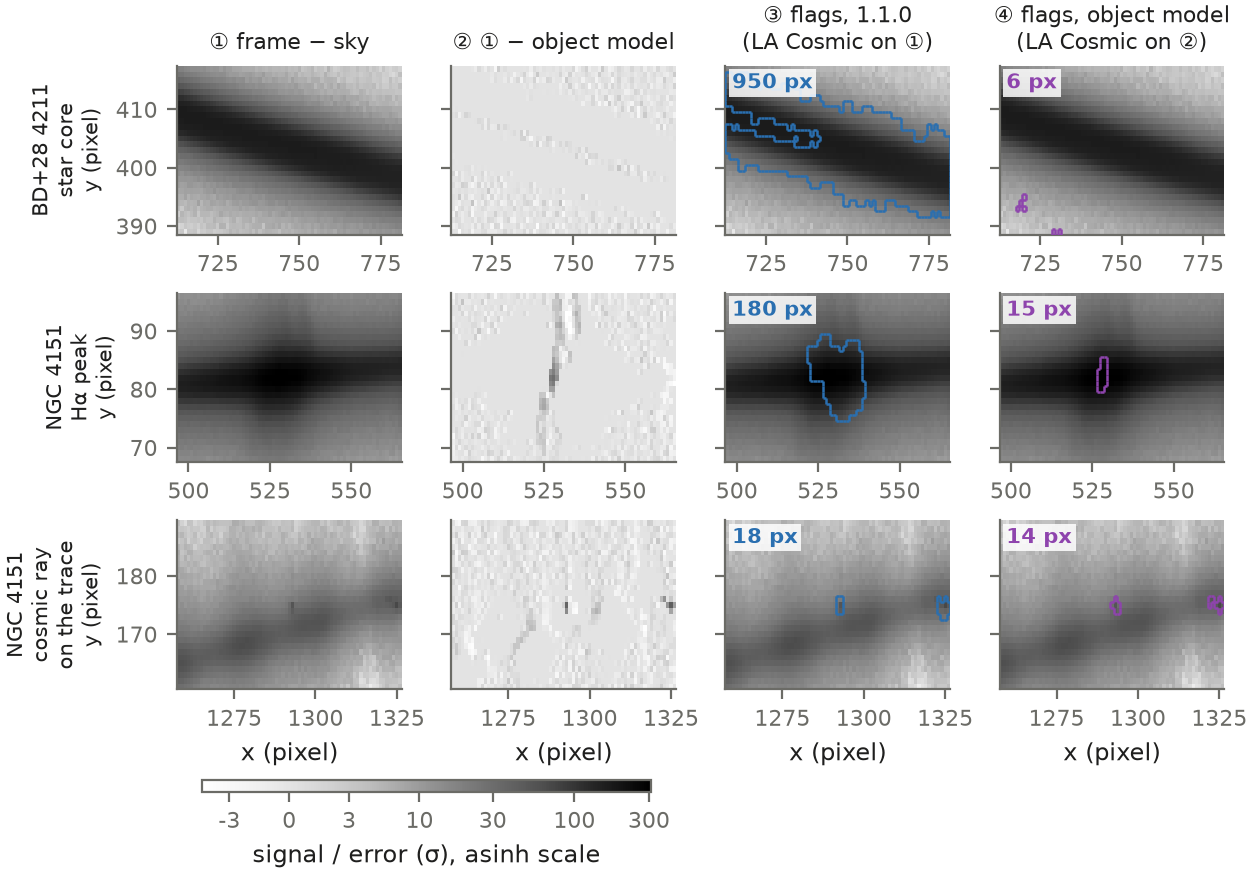
\includegraphics[width=\textwidth]{figures/fig_cr_method.png}
\caption{The change step by step on identical inputs. Columns: \ding{172} the frame minus the sky, which the 1.1.0
detector searches; \ding{173} the same minus the object model (the 7-pixel running median along each detector row),
which LA Cosmic searches with the change; both in units of the error, on one grey scale; \ding{174} the pixels flagged
when LA Cosmic is given only the sky (\banzai{}~1.1.0 and improved v3, blue) and \ding{175} when it is given the sky
and the object model (purple), with the number of flagged pixels in the panel. Rows: the core of BD$+28^\circ4211$ in
1.3\,arcsec seeing (2025 August 19): 950 pixels against 6, all on the sky; the H$\alpha$ peak of NGC\,4151 (2025 July
15): 180 against 15; a real cosmic ray on the trace of NGC\,4151 (2025 July 19), found both ways. The 15 H$\alpha$
pixels still flagged with the object model are false positives, removed by the same-visit check
(Fig.~\ref{fig:cr_pair}).}
\label{fig:cr_method}
\end{figure}

\begin{figure}[!htbp]
\centering
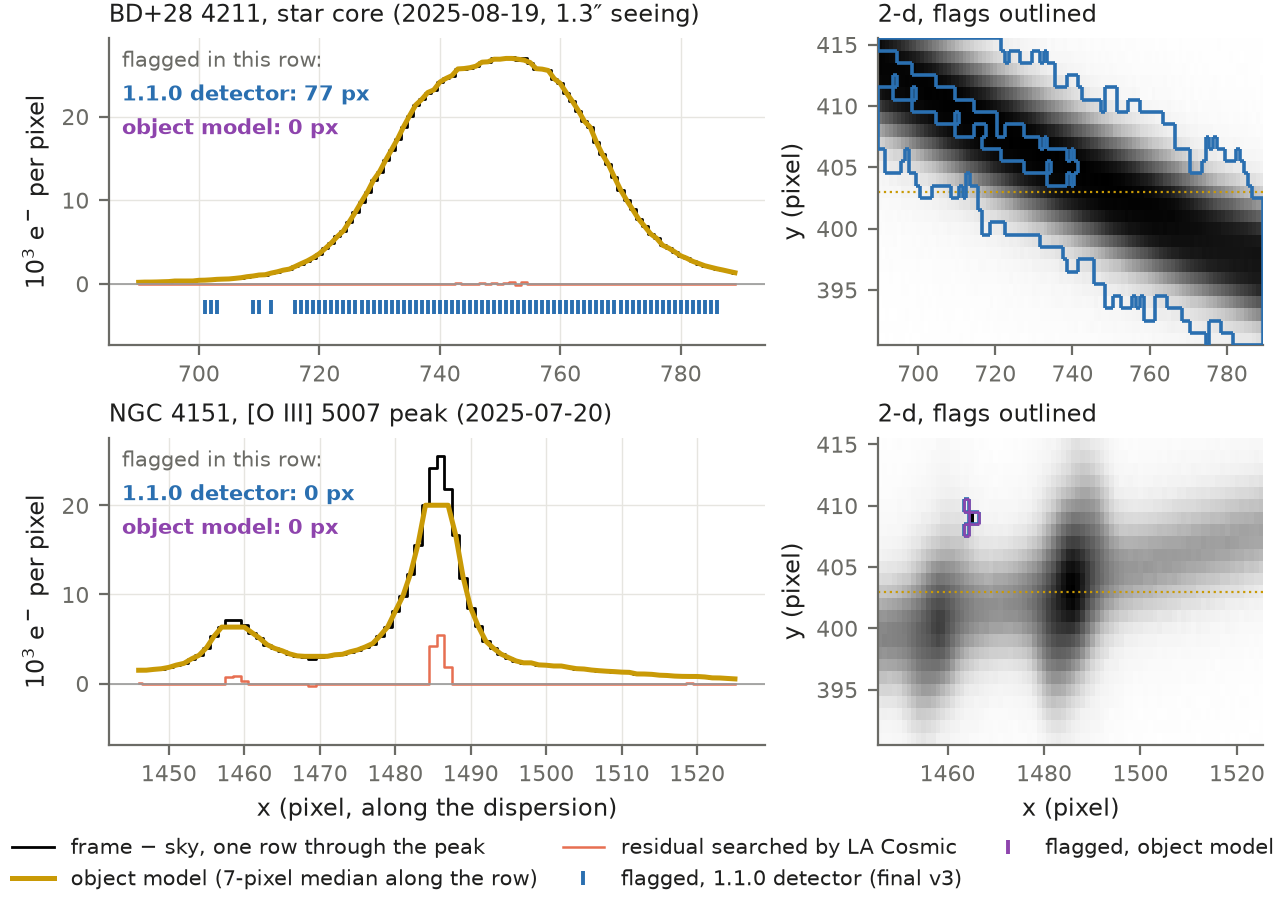
\includegraphics[width=\textwidth]{figures/fig_cr_smoothing.png}
\caption{What the object model does. Left: one detector row through the core of BD$+28^\circ4211$ (top, blue order,
2025 August 19) and through the peak of [O\,{\sc iii}]\,5007 of NGC\,4151 (bottom, 2025 July 20): frame minus sky
(black), the object model, a 7-pixel median along the row (gold), the residual that LA Cosmic searches (orange), and
the pixels flagged in that row by the 1.1.0 detector of improved v3 (blue ticks) and with the object model (purple
ticks); the counts are written in the panel. Right: the 2-d frame (arcsinh grey scale) with the same flags outlined
and the row of the left panel dotted. The flag near $x=1465$ is the warm pixel of the OGG camera, flagged by both.}
\label{fig:cr_smoothing}
\end{figure}

\section{A safety net in the extraction}
\label{sec:cr_guard}
Whatever the detector does, the extraction should not turn a few flagged pixels into a flux error of a factor 2.6. For
each wavelength bin we therefore measure the share of the profile weight in the extraction window ($\sum aP$ of
step 8, Section~\ref{sec:cr_method}) that belongs to pixels flagged as cosmic rays. A single real cosmic ray on the
trace removes at most 0.48 of it (0.15--0.42 for the artificial cosmic rays of Section~\ref{sec:cr_inject}, and 0.48 in
the worst standard star). The clipped H$\alpha$ bins lose 0.51--0.75, even with the new detector. Bins where more than
half of the weight is removed are now masked in the extracted spectrum instead of being scaled up from the rest. We
call this the \textit{extraction guard}. It sets bit 4 of the mask of the extracted spectrum (\texttt{EXTRACTED}
extension), stores the share in a new column \texttt{cr\_masked\_weight}, and counts the masked bins in the header
keywords \texttt{L1QCRB1} and \texttt{L1QCRB2} (red and blue order). A masked bin is not recovered, but it is visible.

% Same-visit cosmic-ray check (banzai_floyds/visit_cosmics.py), input from ch11_cosmics.tex
\section{The second exposure of the visit}
\label{sec:cr_pair}
\textit{The problem.} With the object model, LA Cosmic searches the right residual, but it still has to judge a sharp
feature by its shape alone. A narrow line from a resolved narrow-line region can be as sharp as a cosmic ray (the 15
H$\alpha$ pixels of Fig.~\ref{fig:cr_method}). \textit{The idea.} The visits of the reverberation-mapping programme have
two exposures of the same pointing, taken back to back. A cosmic ray lands in only one of them; a line, a star core, a
sky line or a fringe is in both. The other exposure of the visit (the \textit{partner}) is therefore the most direct
test there is. \textit{The change.} We have added this test to the pipeline as a stage that runs right after LA Cosmic
and that we call the \textit{same-visit check} (code: \texttt{SameVisitCosmicRays} in
\texttt{banzai\_floyds/visit\_cosmics.py}). It removes the LA Cosmic flags on features that the partner also shows,
and adds strong, compact hits that LA Cosmic missed. \textit{Tests and result}
(Sections~\ref{sec:cr_pair_inject} and \ref{sec:cr_pair_sample}): it finds the same artificial cosmic rays as the
object model alone, flags 10--22 per cent fewer pixels, and clears the H$\alpha$ peak of
Fig.~\ref{fig:cr_halpha}.

For a frame $a$ with partner $b$, the check does the following.
\begin{enumerate}
\item \textit{Find the partner}: among the raw frames of the same night in the folder of the frame, those of the same
type and the same LCO \textit{molecule} (the group of exposures taken together within one request; header keyword
\texttt{MOLUID}), the nearest in time first. A frame without a partner keeps the LA Cosmic flags of
Section~\ref{sec:cr_model}. This is the case for all the standards, which are single exposures.
\item \textit{Reduce the partner} up to and including LA Cosmic, in the same way as the frame (no database records are
written for it). Each exposure is sky-subtracted with its own sky model.
\item \textit{Shift the partner along the slit} onto the trace of the frame. The shift is the difference of the fitted
trace centres in each column, smoothed over 15 columns. Where the object is bright (S/N of the column above 30), it is
refined by the difference of the flux centroids within 2\,FWHM of the trace, smoothed over 5 columns. This refinement
is needed because the trace centres follow the continuum, while the narrow-line region of NGC\,4151 can sit up to half a
pixel away, and a half-pixel offset turns the peak of a bright line into a positive--negative pattern in the difference
with the partner.
\item \textit{Scale the partner} in each column by the median ratio $a/b$ over the trace core, smoothed over 31
columns. Where the object is faint, the ratio of the exposure times is used.
\item \textit{Shift the partner along the dispersion.} In a wide slit, the position of the object across the slit
shifts its spectrum. The two exposures of a visit differ by 0.1\,pixel (median) at OGG and 0.3\,pixel at COJ, and by up
to 0.6 and 1.2\,pixels; this puts the flanks of a bright narrow line out of step. The offset is measured for each order
from the cross-correlation of the two spectra summed over the trace (a parabola through its peak). Where it exceeds
0.1\,pixel, it is removed by resampling the partner with a cubic spline. The offset is used only where the peak of the
normalised cross-correlation exceeds 0.5, because a spectrum with no features above the noise has no offset to measure
(Section~\ref{sec:cr_pair_sample}). It is recorded in the header keywords \texttt{L1CRDX1} and \texttt{L1CRDX2} (red
and blue order).
\item \textit{Match the partner to the frame.} The seeing changes within a visit. For example, the FWHM of Fairall\,9
went from 11.6 to 14.7\,pixels between the two exposures of 2026 September 6 (and its flux changed by a factor 0.63);
a scale and a shift cannot absorb that. As in image subtraction \citep{Alard1998}, the partner is therefore convolved
with a kernel along the slit, fitted to the frame:
\[
m(y)=\sum_{|k|\le6}c_k\,s\,b(y+k)+c_{\rm sky}+c'_{\rm sky}\,y ,
\]
where $m$ is the matched partner, $y$ the pixel along the slit, $s$ the scale of step 4, $c_k$ the kernel for an offset
of $k$ pixels, and $c_{\rm sky}$ and $c'_{\rm sky}$ a constant and a slope that absorb a difference between the two sky
models. The kernel is fitted on blocks of 15 columns, on both exposures median-filtered over those columns, with
4$\sigma$ clipping. The median filter is needed for two reasons: a fit on the noisy partner itself is biased towards
zero, and the filter keeps cosmic rays out of the fit. The kernel is then applied to the unfiltered partner, after its
flagged and masked pixels have been replaced by the filtered values. Without this replacement the kernel, which has
negative side lobes when it sharpens the profile, would print a negative copy of a cosmic ray of the partner next to
it. A kernel shared by 15 columns cannot reproduce a hit of a pixel or two, so the matching does not remove real cosmic
rays from the comparison.
\item \textit{Compare}: each pixel gets the significance of its excess over the matched partner,
\[
z=\frac{a-m}{\sqrt{\sigma_a^2+\sigma_m^2+(f\,m)^2}},\qquad f=0.01,
\]
where $\sigma_a$ is the error of the frame, $\sigma_m$ the error of the partner propagated through the kernel, and $f$
a tolerance of 1 per cent for imperfect matching. Each pixel also gets its excess relative to the signal under it,
$r=(a-m)/m$ (with $m$ taken as at least 3 times the denominator of $z$).
\item \textit{Decide}, starting from the LA Cosmic flags. A connected group of flagged pixels is called a
\textit{group}.
\begin{itemize}
\item \textit{Confirm or remove.} A group is \textit{confirmed} if its largest $z$ is at least 3. Otherwise the partner
shows the same feature, and the group is \textit{removed}.
\item \textit{Trim.} Of a confirmed group, only the pixels with $z\ge3$ and their neighbours stay flagged. This prevents
a line peak that LA Cosmic merged with a cosmic ray beside it from being clipped with it.
\item \textit{Pixels the partner cannot check.} Such a pixel always stays flagged, and a group made mostly of such pixels
stays flagged in full. The partner cannot check a pixel that is masked in it; a pixel that it also flags, if the pixel
is off the object (this is how a warm pixel looks); a pixel at the edge of an order; or a pixel where the matched
partner differs from the frame over an extended area (the median of $|z|$ over $5\times5$ pixels is above 2). Such
extended differences occur because the residual 2-d fringes of the red order stay at the same place on the detector
while the partner is shifted onto the trace of the frame, and because the match can fail at the end of an order. A
cosmic ray is compact, so an extended difference says nothing about one. This affects 0.04--4 per cent of an order in
the frames we examined (header keyword \texttt{L1CRMISM}).
\item \textit{Pixels flagged in both exposures, on the object.} LA Cosmic flags the same sharp line and trace peaks in
both exposures of a good-seeing visit. If neither exposure could check the other, both would keep these false flags.
Therefore, on the object (within 2\,FWHM of the trace), a pixel that the partner also flagged is still compared with
the partner's own value, with the kernel applied to the partner without the replacement of step 6. If the two agree,
the pixel holds the same feature in both exposures, since a cosmic ray does not hit the same pixel twice, and the flag
is removed. If the partner is brighter by more than 3$\sigma$, the partner was hit there, and the pixel counts as one
the partner cannot check. No new flags are added on such pixels. Off the object this rule does not apply: a warm pixel
is also in both exposures, and on the sky nothing distinguishes it from a real feature. The header keyword
\texttt{L1CRSHAR} counts the pixels the rule is applied to.
\item \textit{New groups}, the cosmic rays LA Cosmic missed, must pass a stricter test than confirmations, because on a
bright line a mismatch of 1 per cent of the partner is already many $\sigma$. A new group starts from a pixel that
meets all of the following: $z>8$; $r>0.5$, i.e.\ at least 50 per cent above the signal under it; significantly
positive itself, $a>5\sigma_a$ (a cosmic ray adds charge); and at least 6 pixels from the edges of an order along the
slit and from its ends along the dispersion. The group is then extended into neighbouring pixels with $z>3$ and
$a>2\sigma_a$. It is accepted only if the result is compact: at most 30 pixels, 3 pixels thick and 15 long.
\end{itemize}
\end{enumerate}
The result is recorded in the header of every product:
\begin{itemize}
\item \texttt{L1CRMETH}: \texttt{pair} if the frame was checked against a partner, \texttt{lacosmic} if not;
\item \texttt{L1CRPART}: the file name of the partner;
\item \texttt{L1CRNLA}: the number of pixels flagged by LA Cosmic;
\item \texttt{L1CRKEEP}, \texttt{L1CRDROP}, \texttt{L1CRUNCH} and \texttt{L1CRADD}: the number of groups confirmed,
removed, kept because the partner could not check them, and added;
\item \texttt{L1CRNPX}: the number of pixels flagged at the end;
\item \texttt{L1CRMISM}: the fraction of the orders that the partner cannot judge because of extended differences;
\item \texttt{L1CRSHAR}: the number of pixels on the trace flagged by LA Cosmic in both exposures and judged against
the partner's own values;
\item \texttt{L1CRDX1} and \texttt{L1CRDX2}: the offset of the partner along the dispersion, in pixels, for the red and
blue orders.
\end{itemize}

\textit{The tolerance $f$} was measured, not chosen. We used the trace cores of two pairs: the bright NGC\,4151 visit
of 2025 July 14 at OGG (FWHM 4.6 and 4.9\,pixels) and the Fairall\,9 visit of 2026 September 6 described above. If the
errors are right, the robust scatter of $z$ should be 1 (Table~\ref{tab:cr_pair_tol}). With $f=0$, $z$ scatters by
0.8--1.1 at every signal level up to $3\times10^4$\,e$^-$ per pixel (up to 1.4 at COJ, where the object is faint), and
by 1.1--1.2 above that. With $f=0.01$ the scatter of the brightest pixels falls to 0.7, and 0.1 per cent of the core
pixels have $|z|>3.8$--4.1. Without the kernel, $z$ scatters by up to 2.9 (OGG) and 3.4 (COJ) even with a 2 per cent
tolerance, mostly because of the change of seeing. Our first version used tolerances of 5 per cent in flux and
0.25\,pixel in position, chosen by hand to absorb that change. With them $z$ scattered by only about 0.3 on bright
pixels, which hid the weaker hits on bright lines from the comparison.

\begin{table}[!htbp]
\centering\small
\caption{Robust scatter of $z$ on the trace core of two clean pairs, by the signal of the matched partner (e$^-$ per
pixel), with the tolerance adopted ($f=0.01$; partner shifted along the dispersion and matched by the kernel). It
should be 1. The numbers before the arrow are for a scale and a shift along the slit only, with $f=0.02$.}
\label{tab:cr_pair_tol}
\begin{tabular}{lccccc}
\toprule
Pair (frame vs partner) & $<10^3$ & $10^3$--$3\times10^3$ & $3\times10^3$--$10^4$ & $10^4$--$3\times10^4$ & $>3\times10^4$\\
 & \multicolumn{5}{c}{signal of the matched partner (e$^-$ per pixel)} \\
\midrule
NGC\,4151 OGG, 0002 vs 0001 & 1.29$\to$0.83 & 2.17$\to$0.90 & 2.92$\to$0.91 & 1.63$\to$0.83 & 2.60$\to$0.73\\
NGC\,4151 OGG, 0001 vs 0002 & 1.15$\to$0.85 & 1.31$\to$0.84 & 1.53$\to$0.85 & 1.02$\to$0.81 & 1.22$\to$0.66\\
Fairall\,9 COJ, 0014 vs 0013 & 1.93$\to$1.00 & 2.49$\to$0.76 & -- & -- & --\\
Fairall\,9 COJ, 0013 vs 0014 & 1.86$\to$1.02 & 3.44$\to$0.93 & --$\to$1.31 & -- & --\\
\bottomrule
\end{tabular}
\end{table}

\textit{What the tests found while building the check.} Each step above was added because a test failed without it,
and each failure now has its own unit test (16 tests in \texttt{tests/test\_visit\_cosmics.py}).
\begin{enumerate}
\item[(i)] The first version (scale and shift only, with the hand-set tolerances of 5 per cent and 0.25\,pixel) lost
weak hits on bright line peaks in the injection test. The tolerances were hiding the change of seeing; matching the
seeing (step 6) fixed that.
\item[(ii)] The kernel printed negative copies of the partner's cosmic rays: 12 false groups in one Fairall\,9 frame.
Replacing those pixels before the convolution fixed it.
\item[(iii)] A warm pixel flagged in both exposures was unflagged in one of them, because its neighbours, which the
partner could check, agreed. Such pixels now always stay flagged.
\item[(iv)] The first run on the whole sample \textit{added} flags on the narrow lines of NGC\,4151 (840 pixels in 41
of 60 frames), more than the object model alone. Three effects produced excesses that the first, loose rule for new
groups ($z>6$ and 10 per cent above the signal) took for cosmic rays: the offsets along the dispersion; an empty frame
compared with a partner that the kernel had made negative at the order edges; and the unmatched 2-d fringes. The
answers are the shift along the dispersion (step 5), the stricter rule for new groups, and the exclusion of extended
differences. On the four worst frames, the flags on the lines went from 9--23 pixels with the object model to 0--6
kept or added pixels, except in one frame (2025 June 10), where 21 LA Cosmic pixels on the lines are kept and 5 added.
\item[(v)] The run of that version on the whole sample still left 215 flagged pixels on the lines of NGC\,4151, a
hundred times the rate on the continuum next to them, and often on the same line in both exposures of a visit. The
partner had flagged the same peak, so neither exposure could check the other. The rule for pixels flagged in both
exposures on the object is the answer (Section~\ref{sec:cr_pair_sample}). Applied everywhere, the rule also unflagged
warm pixels on the sky, which is why it stops at 2\,FWHM from the trace.
\end{enumerate}
Two refinements that looked right on simulations were measured on the real pairs and dropped: a kernel along the
dispersion, which made the tails of the distribution of $z$ worse, and a wider median filter for the kernel along the
slit, which followed the change of the profile along the order too coarsely.

\begin{figure}[!htbp]
\centering
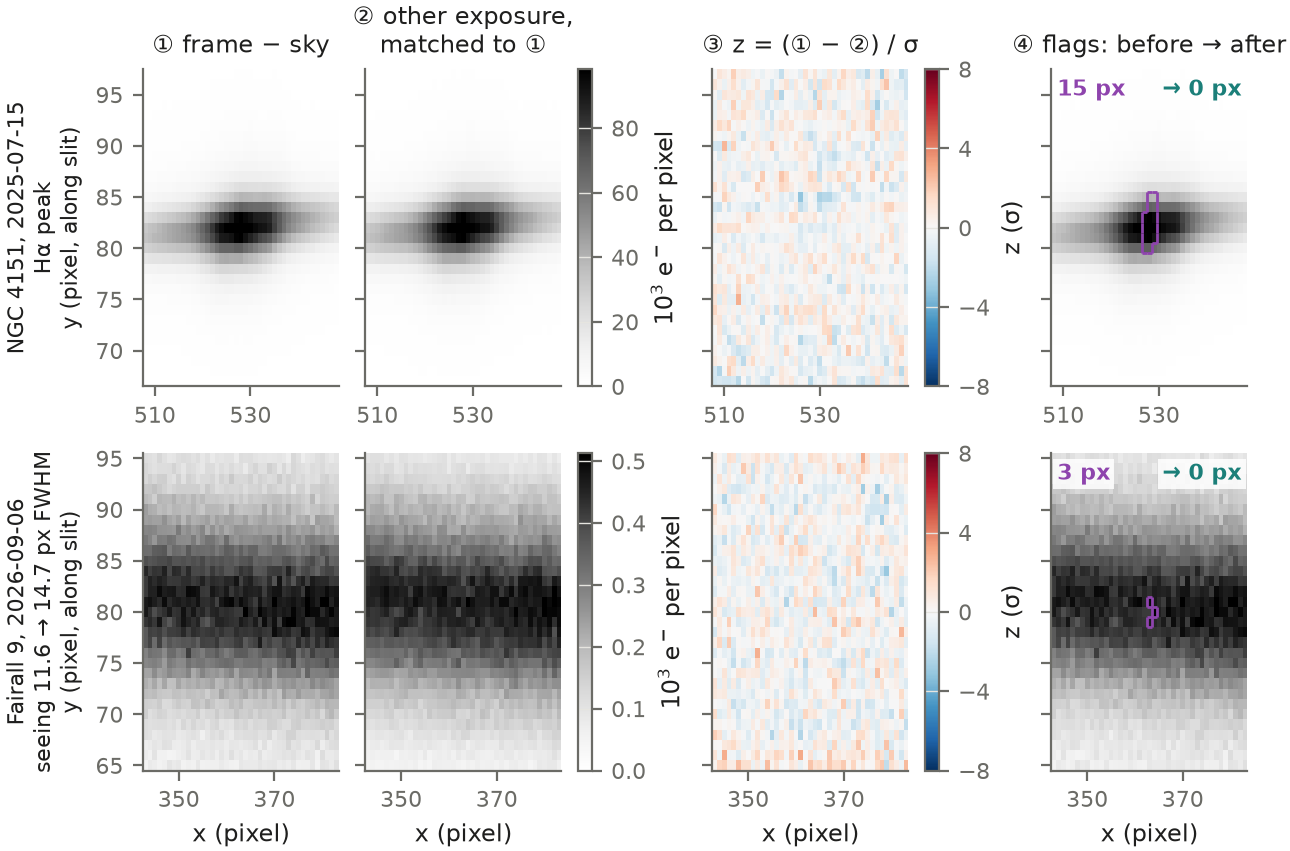
\includegraphics[width=\textwidth]{figures/fig_cr_pair.png}
\caption{The same-visit check on real pairs, both exposures reduced exactly as the stage sees them. Columns:
\ding{172} the frame minus its sky; \ding{173} the partner minus its sky, shifted onto the trace of the frame, scaled
per column, shifted along the dispersion and matched to the frame by the kernel along the slit (same grey scale as
\ding{172}); \ding{174} $z=($\ding{172}$-$\ding{173}$)/\sigma$, which is noise only where the two exposures show the
same thing; \ding{175} the flags of LA Cosmic with the object model (purple, before the check) and those left after the
check (teal; none here), with the number of flagged pixels in the panel. Rows: the H$\alpha$ peak of NGC\,4151 on 2025
July 15 (Figs.~\ref{fig:cr_halpha}, \ref{fig:cr_method}), 15 pixels removed; an LA Cosmic group on the trace of
Fairall\,9 that the partner shows to be real structure, in the visit where the FWHM changed from 11.6 to
14.7\,pixels, 3 pixels removed.}
\label{fig:cr_pair}
\end{figure}

% Results of the same-visit check (input from cr_pair.tex)
\subsection{Injection test with a partner}
\label{sec:cr_pair_inject}
We repeated the injection test of Section~\ref{sec:cr_inject} on eight frames that have a partner: four of NGC\,4151
at OGG and four of Fairall\,9 at COJ. In each frame we placed two random sets of 20 artificial cosmic rays in each of three
places: on the sky, on the trace, and on the line peaks or core. As real cosmic rays
are, they were injected into one exposure of the visit only. Each frame was then reduced three ways: with the 1.1.0
detector, with LA Cosmic and the object model, and with the object model followed by the same-visit check
(Table~\ref{tab:cr_pair_inject}).

\begin{table}[!htbp]
\centering\small
\caption{Injection test on frames with a partner: fraction of injected hits found (any pixel flagged), all hits and
those above 10 times the noise of their pixel, and the cosmic-ray pixels flagged in the same four frames without
injection. 160 hits per category and site (153 on the OGG peaks).}
\label{tab:cr_pair_inject}
\begin{tabular}{llccccc}
\toprule
Site & Detector & Sky & Trace & Line peak & Line peak & Pixels flagged \\
 & & & & or core & or core, $>10\sigma$ & without injection \\
 & & \multicolumn{4}{c}{(fraction of the hits detected)} & (pixels, 4 frames) \\
\midrule
OGG & 1.1.0 / improved v3 & 0.89 & 0.59 & 0.14 & 0.27 & 1037\\
    & object model & 0.89 & 0.76 & 0.50 & 0.89 & 1020\\
    & object model + same visit & 0.89 & 0.76 & 0.50 & 0.89 & 799\\
\midrule
COJ & 1.1.0 / improved v3 & 0.90 & 0.94 & 0.68 & 0.94 & 1775\\
    & object model & 0.90 & 0.94 & 0.79 & 1.00 & 1816\\
    & object model + same visit & 0.90 & 0.94 & 0.78 & 1.00 & 1634\\
\bottomrule
\end{tabular}
\end{table}

\textit{Result.} With the strict rule for new groups, the check finds the same artificial cosmic rays as the object
model alone. Of the 953 hits, none is found only with the check, and 2 are found only without it; both are faint hits on
Fairall\,9 line peaks (3.7--5$\sigma$, 7--12 per cent of the line). On the OGG line peaks, 8 hits above 10$\sigma$ are
missed by both; they carry 4--38 per cent of the line under them. An earlier version of the check, with the loose rule
for new groups, found 14 more hits on the sky and 6 more on the line peaks. But the same rule added hundreds of false
pixels on the narrow lines of the real sample (Section~\ref{sec:cr_pair}, item (iv)), and we chose clean lines.

What the check does is remove flags. In the frames without artificial cosmic rays it flags 22 per cent fewer pixels at
OGG and 10 per cent fewer at COJ. Per frame, it removes 9--19 LA Cosmic groups that the partner shows to be real
structure and adds 0--1; 35--51 groups per frame stay flagged because the partner cannot check them.

These runs were made before the rule for pixels flagged in both exposures on the object was added. That rule acts only
where the partner flagged the same pixel, and an artificial cosmic ray is in one exposure only, so the rule does not
change which of them are found.

\input{chapters/cr_pair_sample}



\section{Verification}
\label{sec:cr_verify}
A detector can always be tuned to look right on the cases it was tuned on, so the changes were tested on a sample they
were not tuned on, in two ways, and compared with the detector of final v3 (that of \banzai{}~1.1.0). The sample was
re-reduced from raw with the new code into a separate folder (the products of this report are unchanged): all 30 visits
of NGC\,4151 (60 frames), 23 visits of Fairall~9 (46 frames; all visits with a quality flag plus a random selection of
the others) and the 12 BD$+28^\circ4211$ frames with flagged cores. The new code includes the sky-line change of
Section~\ref{sec:cr_sky}, so the COJ frames with the noisy sky change for that reason too.

\subsection{Same-visit test}
\label{sec:cr_pairs}
RM visits have two exposures taken minutes apart. A real cosmic ray is in one of them only; a star core, a line or a
detector defect is in both. For each exposure the other one is shifted along the slit to the same trace position
(difference of the fitted profile centres) and scaled column by column to the same brightness (median ratio over the
trace core, smoothed over 31 columns), and each pixel gets the significance of its excess,
$z=(a-sb)/\sqrt{\sigma_a^2+s^2\sigma_b^2+(0.05\,sb)^2}$, where the 5 per cent allows for small changes of seeing and
position between the exposures. Every connected group of flagged pixels is then classified by its pixel of largest
excess: \textit{real} if $z>6$ and the excess is more than 20 per cent of the signal under it, \textit{false positive}
if all its pixels have $z<3$, \textit{detector} if it is equally high in both exposures at the same detector pixel
(a hot pixel, rightly masked), and \textit{ambiguous} otherwise; groups next to a flag of the other exposure are left
out. Unflagged groups of up to 15 pixels with $z>10$ and an excess over 30 per cent on the object count as
\textit{missed}. Figure~\ref{fig:cr_gallery} shows examples of each class. The test has limits: it cannot judge pixels
on the peak of a very bright line, where a few per cent of change between the exposures is many $\sigma$ (the clipped
H$\alpha$ of Fig.~\ref{fig:cr_halpha} comes out ``ambiguous'', and its flux, not its pixels, shows it was clipped), and
the scaling fails when the seeing changes strongly within a visit (2024 November 30, 11\,arcsec seeing, accounts for
most of the ``missed'' groups of OGG with both detectors).

\begin{figure}[!htbp]
\centering
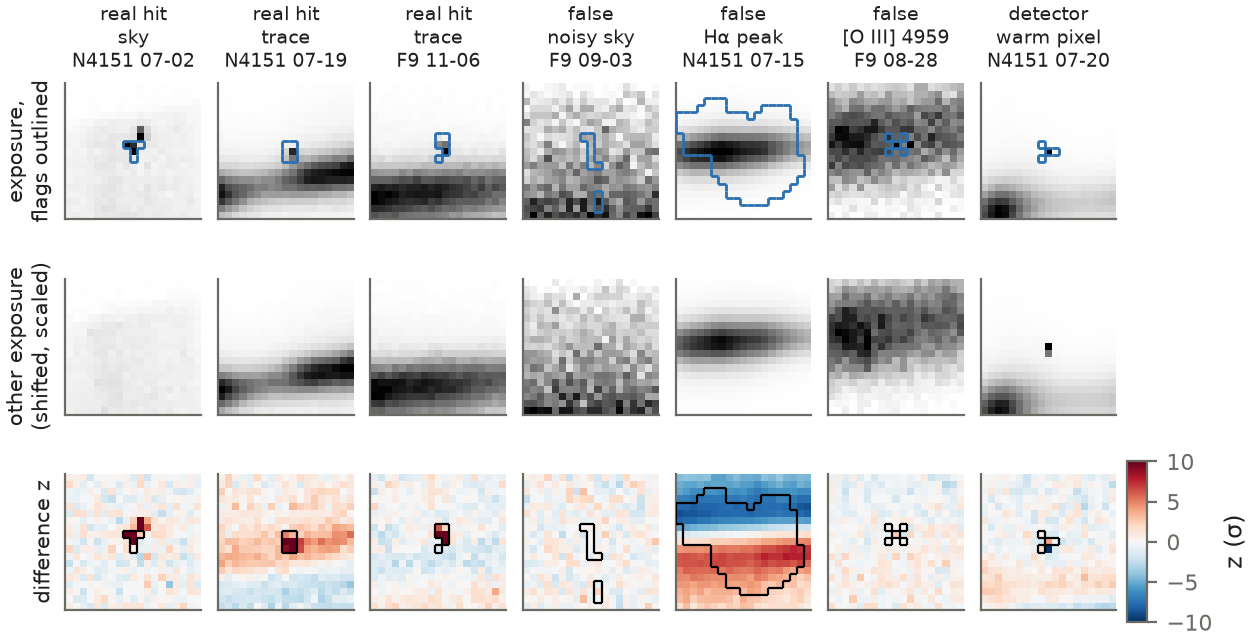
\includegraphics[width=\textwidth]{figures/fig_cr_gallery.png}
\caption{Flagged groups of final v3 classified by the same-visit test. Top: the exposure, flags outlined in red.
Middle: the other exposure of the visit, shifted and scaled onto the first. Bottom: the significance $z$ of the
difference ($-10$ blue to $+10$ red), flags outlined in black. Columns: real hits on the sky and on the trace (a compact
excess absent from the other exposure); false positives from the noisy sky model, on the H$\alpha$ peak (no localised
excess, only the dipole of a sub-pixel shift between the exposures) and on [O\,{\sc iii}]\,4959; and the warm pixel of
the OGG camera, present in both exposures.}
\label{fig:cr_gallery}
\end{figure}

\begin{table}[!htbp]
\centering
\caption{Same-visit test: flagged groups per frame (mean; median in brackets) by class and region, for the detector of
final v3 (\banzai{}~1.1.0) and the new one, on the same frames. ``Object'' is within two FWHM of the trace.}
\label{tab:cr_pairs}
\small
\begin{tabular}{@{}lrrrr@{}}
\toprule
 & \multicolumn{2}{c}{NGC\,4151, OGG (60 frames)} & \multicolumn{2}{c}{Fairall~9, COJ (46 frames)} \\
 & final v3 & new & final v3 & new \\
 & \multicolumn{4}{c}{(groups per frame)} \\
\midrule
real, object & 1.17 (1) & 1.42 (1) & 2.91 (3) & 3.07 (3) \\
false positive, object & 2.72 (1) & 6.30 (5) & 31.2 (6) & 14.8 (10) \\
ambiguous, object & 0.70 (0) & 1.60 (1) & 2.22 (0) & 2.22 (1) \\
missed, object & 11.8 (0) & 11.5 (0) & 1.70 (0) & 1.65 (0) \\
real, sky & 2.35 (2) & 2.35 (2) & 2.54 (2) & 2.65 (2) \\
false positive, sky & 8.87 (9) & 9.53 (9) & 13.2 (9) & 8.46 (8) \\
\bottomrule
\end{tabular}
\end{table}

Table~\ref{tab:cr_pairs} gives the result, and it is mixed:
\begin{itemize}
\item \textit{Real hits} are found as before, slightly more on the object (OGG 70 to 85, COJ 134 to 141 in all), and no
more are missed.
\item \textit{False positives on the object increase in normal frames}: the median per frame goes from 1 to 5 (OGG) and
from 6 to 10 (COJ). The COJ total halves (1435 to 680) only because the frames with the noisy sky model, which had
$\approx240$ each, are fixed. The new false positives are small (median 4 pixels), mostly within one FWHM of the trace
(OGG: 21 groups before, 151 after) and on the continuum, not on lines. Their cause is the other side of the change:
with the object subtracted, the fine-structure test of LA Cosmic is computed on the residual, which is small, and no
longer protects the core of a bright object, so the small pixel-scale structure left in the core of a spectrum with
S/N of a few hundred passes it.
\item \textit{False positives on the sky} are unchanged (OGG) or fewer (COJ, the noisy sky model). They are small groups
of a few faint pixels, cost a few pixels of the sky fit and do not affect the extraction.
\end{itemize}

\subsection{Effect on the extracted fluxes}
\label{sec:cr_flux}
What matters is whether the extra flags change the spectra. Table~\ref{tab:cr_flux} gives the agreement between the two
exposures of each visit, which the flags of either detector can only degrade. The new detector leaves it unchanged
within the noise for [O\,{\sc iii}] in the blue order, for H$\alpha$ and for the continuum, and lowers the bin-to-bin
scatter of the spectra slightly. The worst pairs are the same with both detectors and are grey (clouds, slit losses:
the same ratio in every quantity), except that the new detector removes the clipped H$\alpha$ pair (ratio 0.378). It
creates no new outlier.

The exception is [O\,{\sc iii}]\,5007 of NGC\,4151 in the \textit{red} order, where the line lies only 24\,\AA{} from
the blue end of the order and the dichroic cuts the light steeply: there both detectors clip the line in some frames,
the old one in 2 of 60 (17--22 pixels, flux 4--6 per cent low) and the new one in 6 (5--22 pixels, 4--5 per cent
low); everywhere else the two agree to 0.09 per cent. The bins lose less than half of their profile weight, so the
guard does not catch them. Lines within $\approx30$\,\AA{} of an order end should be measured in the other order, as
[O\,{\sc iii}] normally is in the blue.

\begin{table}[!htbp]
\centering
\caption{Agreement between the two exposures of a visit: robust scatter (per cent) of the ratio of their fluxes, and
the median bin-to-bin scatter of the spectra over their errors (\texttt{L1QXJ}).}
\label{tab:cr_flux}
\small
\begin{tabular}{@{}lrrrr@{}}
\toprule
 & \multicolumn{2}{c}{NGC\,4151 (30 visits)} & \multicolumn{2}{c}{Fairall~9 (23 visits)} \\
 & final v3 & new & final v3 & new \\
\midrule
\multicolumn{5}{@{}l}{\textit{Flux ratio of the two exposures, robust scatter (\%)}}\\
{[O\,{\sc iii}]\,5007}, blue order & 1.99 & 1.93 & 6.7 & 6.8 \\
{[O\,{\sc iii}]\,5007}, red order & 1.71 & 2.49 & 6.7 & 6.6 \\
H$\alpha$+[N\,{\sc ii}] & 2.53 & 2.29 & -- & -- \\
continuum 4200--4500\,\AA{} & 1.49 & 1.56 & 3.3 & 3.6 \\
continuum 7400--7550\,\AA{} & 1.48 & 1.55 & 3.0 & 2.8 \\
\multicolumn{5}{@{}l}{\textit{Bin-to-bin scatter over errors (no unit; 1 = correct)}}\\
scatter / errors (median) & 1.33 & 1.31 & 1.13 & 1.10 \\
\bottomrule
\end{tabular}
\end{table}

\subsection{Injection test}
\label{sec:cr_inject}
The same-visit test cannot see hits on bright line peaks, and it measures false positives better than completeness.
We therefore added 720 synthetic cosmic rays to copies of six raw frames (NGC\,4151 2025-07-15 and 2025-07-20,
BD$+28^\circ4211$ 2025-07-28 and 2025-08-19, Fairall~9 2026-09-06 and 2026-10-08; two random sets each), 20 per frame
in each of three places: the \textit{sky} (more than 3\,FWHM from the trace), the \textit{trace} (within 1\,FWHM, away
from the brightest pixels) and the \textit{peak} (the brightest 3 per cent of the trace core: the line peaks of the AGN
and the core of the star). The hits had peak charges from 50 to 20\,000\,e$^-$ (log-uniform) and the shapes of real
ones (one pixel, two pixels or a short track). Each copy, and the frame without hits, was reduced with both detectors;
a hit counts as detected if any of its pixels is flagged. Figure~\ref{fig:cr_validation} and
Table~\ref{tab:cr_inject} give the result:
\begin{itemize}
\item On the \textit{sky} both detectors find the same 90 per cent of the hits above 10$\sigma$ (the misses are the same
21 hits for both, 14 of them in the 2-pixel band at the order edges that is excluded from the search).
\item On the \textit{trace}, above 10$\sigma$, the old detector finds 89 per cent and the new one 100 per cent.
\item On the \textit{peaks} the old detector finds only 66 per cent of the hits above 10$\sigma$, and in the brightest
frames almost none: of the hits above 20$\sigma$, 0 of 8 on the core of BD$+28^\circ4211$ (2025 July 28) and 2 of 10 on
the H$\alpha$ peak of NGC\,4151 (2025 July 15). The new detector finds 97 per cent (83--100 per cent in every frame).
\item The masks cover the hits equally (95--97 per cent of the pixels of a detected hit), and when hits are added the
old detector also flags 49 pixels per frame that are not on a hit, the new one 13: with the low growth threshold
(step 6), a detection near a bright region spreads into it.
\end{itemize}
The reason is the same as for the false positives above, seen from the other side: the fine-structure test that
protected the object also hid the cosmic rays on it, because a hit on a bright core or line is a small sharp excess on
a large sharp signal. With the object subtracted, the hit stands out. A single hit on the [O\,{\sc iii}] peak of NGC\,4151
missed by the new detector in a first test (Section~\ref{sec:cr_model}) was one of the 3 per cent.

\begin{table}[!htbp]
\centering
\caption{Injection test: fraction of the injected cosmic rays detected (720 hits in six frames, each reduced with both
detectors).}
\label{tab:cr_inject}
\small
\begin{tabular}{@{}lrrrr@{}}
\toprule
 & \multicolumn{2}{c}{hits above 10$\sigma$} & \multicolumn{2}{c}{hits of 5--10$\sigma$} \\
place & final v3 & new & final v3 & new \\
 & \multicolumn{4}{c}{(fraction of the hits detected)} \\
\midrule
sky (240 hits) & 0.90 & 0.90 & 0.92 & 0.92 \\
trace (240) & 0.89 & 1.00 & 0.47 & 0.60 \\
line peak or star core (234) & 0.66 & 0.97 & 0.19 & 0.67 \\
\midrule
flags not on a hit (pixels per frame) & 49 & 13 & & \\
\bottomrule
\end{tabular}
\end{table}

\begin{figure}[!htbp]
\centering
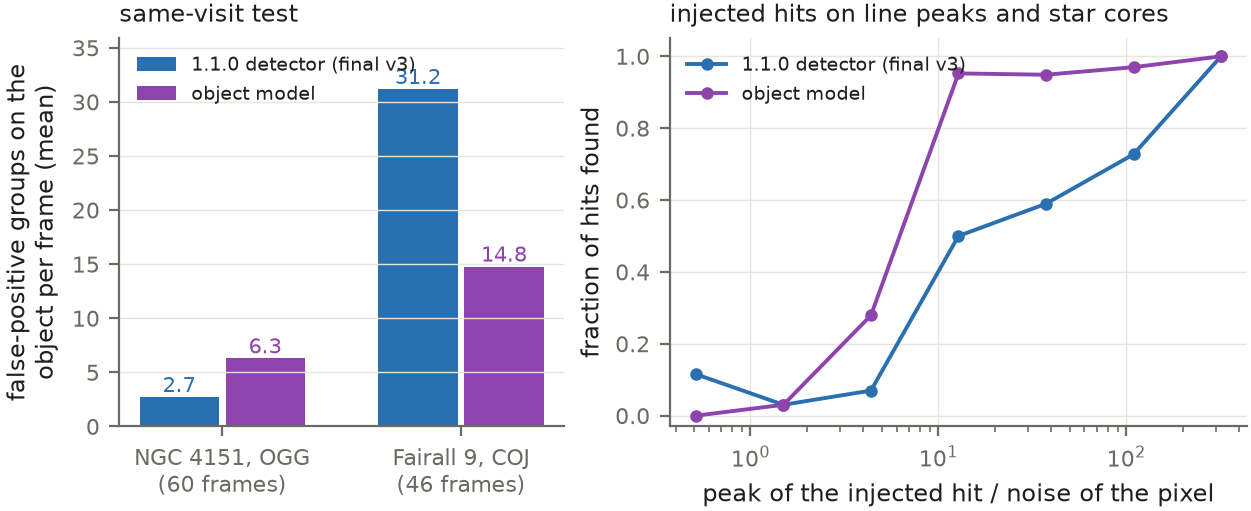
\includegraphics[width=\textwidth]{figures/fig_cr_validation.png}
\caption{Verification of the new detector against that of final v3 (\banzai{}~1.1.0). Left: same-visit test, flagged
groups per frame by class and region (Table~\ref{tab:cr_pairs}; the many ``missed'' groups of OGG are one visit with
11\,arcsec seeing, for both detectors). Middle: fraction of injected hits detected against their significance, on the
sky (dotted), the trace (dashed) and the line peaks or star core (solid), old (red) and new (blue). Right: the same
against the ratio of the hit to the signal under it, for hits above 10$\sigma$.}
\label{fig:cr_validation}
\end{figure}

\subsection{Conclusion}
\label{sec:cr_conclusion}
On the object, the new detector finds more of the real cosmic rays (on bright cores and line peaks 97 instead of 66 per
cent), stops flagging the cores of bright stars (46 to 0.1 per cent) and most of the clipped H$\alpha$ (179 to 15 pixels;
flux error 2.64 to 1.02), and removes the false detections caused by a noisy sky. In exchange it adds a few small false
detections per frame on the trace of bright objects (median 1 to 5 at OGG), which leave the extracted fluxes unchanged
within the noise, except for lines within $\approx30$\,\AA{} of an order end, where both detectors clip (2 and 6 frames of
60). On balance it is better on every measure that affects the spectra, but it is not perfect, and the results depend
on the parameters of LA Cosmic, which were left as in \banzai{}. A single frame cannot reliably separate a cosmic ray
from the peak of a bright line; the two or more exposures of every RM visit can, and comparing them is the robust
solution we recommend (Chapter~\ref{sec:recommendations}). We have not re-reduced the products with the new detector:
that, and whether to adopt it before a comparison of exposures exists, is a decision for the team.



\section{Quality keywords in every product}
\label{sec:qc}
Each science and standard product now carries per-frame quality keywords, whose names start with \texttt{L1Q}. They
are in the primary header of the \texttt{-1d} file and in the \texttt{SCI} header of the \texttt{-2d} file. A bitmask,
\texttt{L1QFLAG}, marks the problems found, and \texttt{L1QFLAGS} lists the names of the flags set
(Table~\ref{tab:qc_flags}). The last stage of the pipeline writes them. For products already on disk, the command
\texttt{banzai\_floyds\_qc} computes the same values from the files and writes them into the headers. It also writes a
table with one row per product, to be joined to a master table on the file name. The table holds all \texttt{L1} and
\texttt{L1Q} keywords and the observing conditions already in the headers of the raw frames: the guider seeing
(\texttt{AGFWHM}), the airmass (\texttt{AIRMASS}), the illuminated fraction of the Moon and its distance from the target
(\texttt{MOONFRAC}, \texttt{MOONDIST}) and the cloud measure of the weather station (\texttt{WMSCLOUD}). We added the
keywords to all 317 science and standard products of improved v3 at both sites. Their definitions and normal ranges are
in the file \texttt{docs/QC\_KEYWORDS.md} of the package. We set the thresholds of the flags just outside the normal
range of these reductions and checked them against the frames found by hand in this report.

The keywords are (a trailing 1/2 means one keyword for each order, red and blue):
\begin{itemize}
\item \texttt{L1QSN1/2}: the median S/N per wavelength bin.
\item \texttt{L1QXJ1/2}: the bin-to-bin scatter of the extracted flux over its errors. It is the robust rms of the
second difference of the flux divided by its expected error: 1 for pure noise, and insensitive to a smooth spectrum.
\texttt{L1QBJ1/2} is the same for the sky model under the object, still over the flux errors.
\item \texttt{L1QCR1/2}: the per cent of the trace core (pixels within one FWHM of the trace) flagged as cosmic rays.
\item \texttt{L1QCRLN}: cosmic-ray flags on the trace core of strong narrow emission lines. The lines are found in the
spectrum itself, as bins well above a running median, so no redshift is needed.
\item \texttt{L1QCRB1/2}: bins masked by the extraction guard (Section~\ref{sec:cr_guard}).
\item \texttt{L1QSEE1/2}: the seeing measured in the slit, the FWHM of the fitted spatial profile. (The guider's
\texttt{AGFWHM} is missing or zero in some frames.)
\item \texttt{L1QPOFF}: the offset of the object along the slit.
\item \texttt{L1QSTDGR}, standards only: the light collected relative to the clear ensemble of the other standards. It
finds standards taken through clouds and failed acquisitions.
\item \texttt{L1QSTDDT} and \texttt{L1QSTDSP}, science frames only: the days to the nearest and to the farthest standard
of the flux ensemble.
\end{itemize}

\begin{table}[!htbp]
\centering
\caption{Quality flags (\texttt{L1QFLAG} bits) and how many products of improved v3 have each. ``Science''
includes EG\,21 at COJ, which is not in the standards catalogue. A product can have several flags. ``Trace core'' is
the pixels within one FWHM of the trace; the refraction scale is a parameter of the physical trace model
(Chapter~\ref{sec:traces}); in the \texttt{BKMASK} row $\sigma$ is the width of the spatial profile.}
\label{tab:qc_flags}
\small
\begin{tabular}{@{}rlp{6.4cm}rrrr@{}}
\toprule
 & & & \multicolumn{2}{c}{COJ} & \multicolumn{2}{c}{OGG} \\
bit & flag & set when & sci. & std. & sci. & std. \\
 & & & \multicolumn{4}{c}{(number of products)} \\
\midrule
1 & \texttt{XJIT} & flux scatter $>2.5\times$ errors (either order) & 5 & 0 & 0 & 1 \\
2 & \texttt{BKJIT} & sky-model scatter $>1\times$ flux errors & 9 & 0 & 0 & 0 \\
4 & \texttt{CRCORE} & $>1$ per cent of the trace core flagged as cosmic rays & 0 & 0 & 0 & 12 \\
8 & \texttt{CRLINE} & $\geq3$ flags on the core of strong narrow lines & 5 & 0 & 3 & 0 \\
16 & \texttt{LOWSNR} & median S/N per bin $<10$ & 0 & 0 & 0 & 0 \\
32 & \texttt{TRACE} & trace not from the physical model, or $|$refraction scale$|>3$ & 0 & 0 & 0 & 1 \\
64 & \texttt{PROFILE} & profile width not fitted & 0 & 0 & 0 & 1 \\
128 & \texttt{BKMASK} & object mask narrowed below 6$\sigma$ (wide object, little sky) & 17 & 4 & 1 & 1 \\
256 & \texttt{STDGREY} & standard collected $<0.5$ of the clear ensemble & -- & 2 & -- & 4 \\
512 & \texttt{STDFAR} & nearest standard $>5$ days away & 44 & -- & 8 & -- \\
1024 & \texttt{FRINGE} & fringe residual ratio $>0.75$ & 0 & 0 & 0 & 1 \\
2048 & \texttt{NOOBJ} & no object detected & 0 & 0 & 0 & 0 \\
4096 & \texttt{SEEING} & seeing $>1.5\times$ the slit width & 9 & 21 & 0 & 10 \\
8192 & \texttt{CRBIN} & bins masked by the extraction guard & -- & -- & -- & -- \\
\midrule
 & \texttt{OK} & no flag & 58 & 18 & 48 & 75 \\
 & & products & 118 & 39 & 60 & 100 \\
\bottomrule
\end{tabular}
\end{table}

The flags find the problems of this chapter and of the earlier ones:
\begin{itemize}
\item \texttt{XJIT} and \texttt{BKJIT} find the Fairall~9 frames with the noisy sky model, and \texttt{XJIT} also the
BD$+28^\circ4211$ frame with half its core flagged.
\item \texttt{CRCORE} finds only BD$+28^\circ4211$, and \texttt{CRLINE} the clipped H$\alpha$.
\item \texttt{STDGREY} finds GD\,153 on 2025 May 25 (0.09 of the light of the clear standards; also flagged
\texttt{TRACE}, \texttt{PROFILE} and \texttt{FRINGE}), BD$+28^\circ4211$ on 2025 August 10 (0.06), and four standards
taken through clouds.
\item \texttt{STDFAR} shows that 44 COJ science frames are more than five days from a catalogue standard, because only
Feige\,110 is in the catalogue. EG\,21, taken almost every night, would close the gap
(Chapter~\ref{sec:recommendations}).
\item \texttt{CRBIN} is zero in all these products, because the extraction guard did not exist when they were reduced.
\end{itemize}

\begin{table}[!htbp]
\centering
\caption{Status of the changes of this chapter.}
\label{tab:cr_status}
\small
\begin{tabular}{@{}p{5.2cm}p{3.6cm}p{5.6cm}@{}}
\toprule
Change & In the code & In the products of this report \\
\midrule
Sky lines must stand out from the first-pass scatter & yes, tested & no: re-reduction pending \\
Object model for LA Cosmic & yes, tested & no: re-reduction pending \\
Extraction guard (mask bit 4) & yes, tested & no: re-reduction pending \\
Same-visit check after LA Cosmic & yes, tested (16 unit tests, 106 frames) & no: re-reduction pending \\
Gaia lookup tries a second VizieR mirror & yes, tested & no: re-reduction pending \\
Quality keywords & yes (last stage) & yes, added with \texttt{banzai\_floyds\_qc} \\
Warm pixel of the OGG camera in the bad-pixel mask & no & no \\
\bottomrule
\end{tabular}
\end{table}

\chapter{Recommendations}
\label{sec:recommendations}

\textit{For observers and LCO operations.}
\begin{enumerate}
\item \textit{Flux standards throughout every campaign}, of stars in the \banzai{} catalogue, at least every few nights.
The ensemble calibration needs standards on both sides of every science frame, and at OGG a throughput change of a
factor 1.8 in 2025 April could only be bridged because standards outside the catalogue (Feige\,67, GD\,153) had been
observed (Section~\ref{sec:sites_flux}). A 6\,arcsec standard now and then would allow a residual fringe template and
a telluric transmission for the RM slit itself.
\item \textit{Log and announce changes of the telescope throughput} (mirror recoating, cleaning, optics changes), so that the
pipeline can be told not to combine standards across them. The re-aluminisation of the FTN mirror in 2025 April
changed the blue-order response by up to 48 per cent relative to the red (Section~\ref{sec:shape_stability}), and it
had to be found in the data.
\item Check the Zn lamp: it is ``on'' in the headers but produces no lines. Zn\,4680, 4722, 4811 and 5182 would fill
the blue-order gap at H$\beta$/[O\,{\sc iii}].
\item Take arcs through a narrow slit (alone or in addition to the 6\,arcsec arcs) for the wavelength solution:
with a 6\,arcsec slit the arc lines are 51\,\AA{} wide top-hats and blend.
\item Same-block lamp flats are useful but not essential for the fringes: the detector pattern is stable over months
and only its phase is used (Section~\ref{sec:fringe_harmonic}). A narrow-slit lamp flat would record the fringe
shape with less smoothing.
\item Observe a standard every night in the same configuration as the science if the absolute spectral shape below
3800\,\AA{} matters: a same-night standard reproduces the shape there to 0.5 per cent, a standard from another night
to 3--5.5 per cent.
\end{enumerate}

\textit{For \banzai{}: done in improved v3} (branch \texttt{rm-improvements}, Chapter~\ref{sec:software}), proposed for
the LCO code.
\begin{enumerate}
\item Hg\,4916 (both orders) and Ar\,6416, 6677, 6753/6767 (red) in the used arc lines (Section~\ref{sec:sites_arcs}).
\item A per-exposure object zero point from the telluric bands, transferred to the blue order (Section~\ref{sec:wl_zp};
pipeline stage \texttt{ObjectWavelengthCorrector}).
\item No 2-d division by a lamp flat: the harmonic fringe model with the lamp phase only, fitted per exposure jointly
with a telluric template, plus a residual template per slit (Chapter~\ref{sec:fringe}).
\item The physical object-trace model with a template per site (Sections~\ref{sec:traces_model} and
\ref{sec:sites_trace}).
\item Telluric transmission applied only inside the absorption bands, from the nine nearest standards; the O$_2$ A band
flagged in science spectra (Section~\ref{sec:flux_tell}).
\item The flux calibration from the grey-normalised median of the nine nearest standards of any slit width
(Section~\ref{sec:flux_ensemble}); Feige\,67 and GD\,153 added to the catalogue (Section~\ref{sec:sites_flux}).
\item Sky flats processed by the LCO archive accepted for locating the orders; offline reduction of a whole data set
with one command (Appendix~\ref{sec:app_install}).
\item Quality keywords and a flag bitmask in every science and standard product (Section~\ref{sec:qc}).
\end{enumerate}

\textit{For \banzai{}: in the code, verified on a sample, products not yet re-reduced} (Chapter~\ref{sec:cosmics}).
\begin{enumerate}
\item Give LA Cosmic, the cosmic-ray detector of \banzai{}, a model of the object as well as the sky, so that the cores of bright stars are not flagged.
\item Mask extracted bins that lose more than half of their profile weight to cosmic-ray flags instead of scaling
them up (a clipped H$\alpha$ was 2.6 times too bright).
\item Treat a feature as a sky line only if it stands out from the noise of a first-pass sky fit, so that the spline
sky model does not follow the noise beside a wide object.
\end{enumerate}

\textit{For \banzai{}: still open.}
\begin{enumerate}
\item Add EG\,21 (and the other nightly standards of COJ and OGG) to the catalogue with references of adequate
resolution; EG\,21 has only the 50\,\AA{} CTIO fluxes (Section~\ref{sec:flux_model}).
\item Do not combine standards across a throughput change: for example, limit the ensemble to a period of constant
throughput, or test the grey levels of the standards in time order for jumps. A mirror recoating changes the shape of
the response as well as its level (Section~\ref{sec:shape_stability}), so the test should look at the colour of the
response too.
\item Leave standards flagged by the quality checks (failed trace or profile) out of the ensemble. The median of nine
absorbs one such standard (Section~\ref{sec:shape_stability}), but a frame calibrated with few standards would not.
\item Model the telluric absorption (a line-by-line transmission with a free water column) at each spectrum's
resolution, which in a wide slit is set by the seeing. The night-to-night change of the water absorption
($\approx3.5$ per cent in the band level) is not followed by a nine-standard median, and the O$_2$ A band can only be
flagged.
\item Anchor the flux and telluric calibration redward of 8900\,\AA, where there is no telluric-free continuum and
both are extrapolated (Appendix~\ref{sec:app_v1}); until then, use the red end with care.
\item Carry the fringe and telluric residuals in the error array, or document a systematic term: the uncertainties
are right per pixel, but integrated quantities need $\approx20$--30 per cent more (Section~\ref{sec:raw_errors}).
\item Provide the two orders as separate products: the combined spectrum mixes the misaligned orders over
4540--5760\,\AA.
\item Write lean 2-d products (or compress \texttt{BINNED2D}, the table of all pixels): a processed 2-d frame is 47\,MB, of which
43\,MB is that table (Section~\ref{sec:sites_disk}).
\item Reject cosmic rays by comparing the exposures of a visit (RM visits have two or more): a real line is in all of
them, a cosmic ray in one. A single frame cannot tell a cosmic ray on the peak of a bright line from the line
(Section~\ref{sec:cr_verify}).
\item Add the warm pixel of the OGG camera at $(1465,409)$ to the bad-pixel mask.
\item The archive products of \banzai{}~1.0.1 are not scaled by the exposure time, so 600\,s science frames calibrated
with 300\,s standards are twice too bright (Section~\ref{sec:flux_banzai}); 1.1.0 is correct. Archive users should be
told.
\end{enumerate}

\chapter{Software}
\label{sec:software}

All code is in our version of \banzai{} (branch \texttt{rm-improvements}; Appendix~\ref{sec:app_install}). The
list below gives, for each Python module of the package \texttt{banzai\_floyds}, what it does and where in this report
it is described; it is meant for readers who want to use or check the code. The diagnostics and archive tools need
only \textsc{numpy}, \textsc{scipy}, \textsc{astropy} and \textsc{matplotlib}.

\begin{description}
\item[\texttt{diagnostics.rm\_qa}] narrow-doublet and single-line fits, sky and telluric shifts, order-overlap ratio
(Chapter~\ref{sec:diagnostics}).
\item[\texttt{diagnostics.sky\_lines}] off-object sky spectrum from \texttt{BINNED2D}; adaptive top-hat centroids.
\item[\texttt{utils.arc\_refit\_utils}] arc refit: arc spectrum collapsed along the slit, line-group model (eqs.~\ref{eq:arcgroup}--\ref{eq:boxcar}),
correction (eq.~\ref{eq:arccorr}).
\item[\texttt{utils.wavelength\_offset\_utils}] telluric zero point (eqs.~\ref{eq:tell}, \ref{eq:tellcomb},
\ref{eq:transfer}).
\item[\texttt{wavelength\_offsets.ObjectWavelengthCorrector}] pipeline stage that applies the telluric zero point
of the object (runs after the extracted spectra are trimmed).
\item[\texttt{diagnostics.reextract}] archive products only (improved v1, Appendix~\ref{sec:app_v1}): undoing the
fringe division, master pattern, lamp-flat matching, harmonic fringe model, sky and extraction (eqs.~\ref{eq:undo}--\ref{eq:boxcarext});
command line \texttt{python -m banzai\_floyds.diagnostics.reextract}.
\item[\texttt{diagnostics.correct\_archive\_wavelengths}] arc refit and telluric zero point on archive
\texttt{-1d} files; console script \texttt{banzai\_floyds\_correct\_wavelengths}.
\item[\texttt{utils.sensitivity\_utils}, \texttt{diagnostics.recalibrate\_flux}] sensitivity as a template times a
nightly correction, and telluric correction, for archive products (eqs.~\ref{eq:sens}--\ref{eq:apply}).
\item[\texttt{utils.trace\_model\_utils}] object-trace model: refraction along the slit, instrumental template,
smooth correction of the residuals (eqs.~\ref{eq:adr}--\ref{eq:tracehybrid}); template in
\texttt{data/orders/trace\_template.dat}.
\item[\texttt{utils.harmonic\_fringe\_utils}] harmonic fringe model (shared by the pipeline and the archive tool),
including the blended phase (high-passed lamp phase in the blue part of the model, plain phase further red;
Section~\ref{sec:fringe_pipeline}).
\item[\texttt{fringe.HarmonicFringeCorrector}] pipeline stage that fits the harmonic fringe model; it runs after the
standards are loaded (stage \texttt{StandardLoader}). The stage \texttt{FringeLoader} supplies the phase from the
phase master.
\item[\texttt{telluric}] transmission applied only in the absorption bands; ensemble of the nearest standards for
science frames (\texttt{utils.telluric\_utils}).
\item[\texttt{flux}, \texttt{utils.flux\_utils}] ensemble flux calibration (grey-normalised median of the nearest
standards).
\item[\texttt{arc\_lines}] used arc lines, now including Hg\,4916 and Ar\,6416, 6677, 6753, 6767 with measured
strengths (\texttt{work/scripts/arc\_line\_strengths.py}).
\item[\texttt{data/standards}] reference spectra; Feige\,67 (extended beyond 9200\,\AA{} with a fitted power law)
and GD\,153 added.
\item[\texttt{offline}, \texttt{fringe\_masters}] offline reduction of a data set; construction of the phase masters
and of the residual fringe templates.
\end{description}
Analysis scripts used for this report (in \texttt{work/}): \texttt{scripts/v3\_verify.py} (step-by-step verification
of a reduction, Section~\ref{sec:sites_verify}), \texttt{scripts/compare\_versions.py} and
\texttt{make\_raw\_compare\_tex.py} (Table~\ref{tab:versions}), \texttt{scripts/build\_trace\_template.py} (trace
template and priors of a site), \texttt{scripts/arc\_check\_v3.py} (arc line-group shifts),
\texttt{v3\_chain.py} (a whole reduction in batches that keep the disk use low) and \texttt{banzai\_run/lean\_2d.py}
(lean 2-d products).
New settings (all defaults of this branch) choose the fringe method and its phase source, nodes, high-pass and
telluric blending; the object-trace model and its priors; and the telluric bands and the number and time span of the
standards in the ensemble: \texttt{FRINGE\_METHOD='harmonic'}, \texttt{FRINGE\_PHASE\_SOURCE='stacked'},
\texttt{FRINGE\_HARMONIC\_NODES}, \texttt{FRINGE\_PHASE\_HIGHPASS}, \texttt{FRINGE\_TELLURIC\_BLEND},
\texttt{PROFILE\_TRACE\_MODEL='adr'}, \texttt{PROFILE\_TRACE\_MODEL\_PRIORS}, \texttt{TELLURIC\_MODEL\_BANDS},
\texttt{TELLURIC\_ENSEMBLE\_N}, \texttt{TELLURIC\_ENSEMBLE\_DAYS}; setting them to the 1.1.0 values
(\texttt{'2d'}, \texttt{'polynomial'}, \texttt{None}) restores the stock behaviour. The offline reduction is the
command \texttt{banzai\_floyds\_offline} (subcommands \texttt{setup-db}, \texttt{skyflats}, \texttt{run},
\texttt{chain}; module \texttt{offline}), and the fringe products are built by \texttt{banzai\_floyds\_make\_phase\_master} and
\texttt{banzai\_floyds\_make\_residual\_template} (module \texttt{fringe\_masters}); Appendix~\ref{sec:app_install}.
From raw, all corrections run inside \banzai{}; \texttt{banzai\_floyds\_offline chain} reduces, in order, the arcs,
lamp flats, phase masters, standards, residual fringe template, the standards again, and the science frames. On
archive products (improved v1) the corrections are applied in this order: re-extraction $\rightarrow$ arc refit $\rightarrow$ telluric zero point $\rightarrow$ flux calibration. Unit tests with synthetic data (\texttt{tests/test\_wavelength\_offsets.py},
\texttt{test\_arc\_refit.py}, \texttt{test\_reextract\_flux.py}, \texttt{test\_trace\_model.py},
\texttt{test\_telluric.py}, \texttt{test\_flux\_ensemble.py}, \texttt{test\_fringe\_masters.py}) cover every new
step; the full suite of the package (176 tests) passes.


\chapter*{Acknowledgements}
\addcontentsline{toc}{chapter}{Acknowledgements and data availability}
Based on observations obtained with the FLOYDS spectrograph on the Faulkes Telescope South (Las Cumbres Observatory).
The EG\,21 reference fluxes are from the ESO/CTIO spectrophotometric standard library \citep{Hamuy1992,Hamuy1994}.
The archive products used here are available from the LCO science archive. The software described in
Chapter~\ref{sec:software} is on the \texttt{rm-improvements} branch of \banzai{} (based on commit \texttt{1f53d3e}).
The diagnosis, the pipeline changes, the tests, the figures and the drafting of this report were carried out with the
assistance of Claude Opus~5.5 (Anthropic; model identifier \texttt{claude-opus-5-5}), used through Claude Code;
all results were checked against the data and the scripts that produce them are listed in
Chapter~\ref{sec:software}.

\begin{thebibliography}{99}
\addcontentsline{toc}{chapter}{References}
\bibitem[Alard \& Lupton(1998)]{Alard1998} Alard C., Lupton R.~H., 1998, ApJ, 503, 325
\bibitem[Cappellari(2017)]{Cappellari2017} Cappellari M., 2017, MNRAS, 466, 798
\bibitem[Fausnaugh(2017)]{Fausnaugh2017} Fausnaugh M.~M., 2017, PASP, 129, 024007
\bibitem[Filippenko(1982)]{Filippenko1982} Filippenko A.~V., 1982, PASP, 94, 715
\bibitem[Hamuy et~al.(1992)]{Hamuy1992} Hamuy M., Walker A.~R., Suntzeff N.~B., Gigoux P.,
  Heathcote S.~R., Phillips M.~M., 1992, PASP, 104, 533
\bibitem[Hamuy et~al.(1994)]{Hamuy1994} Hamuy M., Suntzeff N.~B., Heathcote S.~R., Walker
  A.~R., Gigoux P., Phillips M.~M., 1994, PASP, 106, 566
\bibitem[Horne(1986)]{Horne1986} Horne K., 1986, PASP, 98, 609
\bibitem[Vieliute et~al.(2025)]{Vieliute2025} Vieliute R., et~al., 2025, RASTI, rzaf021
\bibitem[Kelson(2003)]{Kelson2003} Kelson D.~D., 2003, PASP, 115, 688
\bibitem[Matheson et~al.(2000)]{Matheson2000} Matheson T., Filippenko A.~V., Ho L.~C., Barth A.~J., Leonard D.~C.,
2000, AJ, 120, 1499
\bibitem[Oke(1990)]{Oke1990} Oke J.~B., 1990, AJ, 99, 1621
\bibitem[Osterbrock et~al.(1996)]{Osterbrock1996} Osterbrock D.~E., Fulbright J.~P.,
  Martel A.~R., Keane M.~J., Trager S.~C., Basri G., 1996, PASP, 108, 277
\bibitem[Storey \& Zeippen(2000)]{Storey2000} Storey P.~J., Zeippen C.~J., 2000, MNRAS, 312, 813
\bibitem[van Dokkum(2001)]{vanDokkum2001} van Dokkum P.~G., 2001, PASP, 113, 1420
\bibitem[van Groningen \& Wanders(1992)]{vanGroningen1992} van Groningen E., Wanders I., 1992, PASP, 104, 700
\end{thebibliography}

\appendix
\chapter{Recalibrating the archive products (improved v1)}
\label{sec:app_v1}
Before \banzai{} was run from the raw frames, the corrections were developed on the public \texttt{-1d}/\texttt{-2d}
products of \banzai{}~1.0.1. Those products had already been divided by a shifted lamp flat, so the division had to
be undone, the destroyed pixels masked, and the sky and the extraction redone before the fringe model could be applied.
This appendix documents that procedure (improved v1, Table~\ref{tab:versions_names}). It is not part of the pipeline
run from raw (improved v2 and v3), which never divides by a flat and uses \banzai's own sky model and extraction; it
remains useful for reprocessing archive products for which the raw frames are not available
(\texttt{banzai\_floyds.diagnostics.reextract}, Chapter~\ref{sec:software}).

\section{Undoing the division and the master pattern}
\label{sec:fringe_master}
The frame before the division is recovered as
\begin{equation}
R(x,y)=\begin{cases} I(x,y)\,\Phi(x,y) & 0.5<\Phi<2\\ I(x,y) & |\Phi|<10^{-3}\ \text{(not applied)}\\
\text{masked} & \text{otherwise,}\end{cases}
\label{eq:undo}
\end{equation}
with $I$ the \texttt{SCI} image, and likewise for the uncertainty. Each frame's map is the lamp pattern
$\Pi$ shifted along the slit, $\Phi_f(x,y)=\Pi(x,y-o_f)$, so $\Pi$ is recovered by shifting $\Phi_f$ by $-o_f$
(linear interpolation; pixels with interpolation weight $<0.99$ discarded). The 61 maps with $|o_f|<40$ give
patterns that agree with their median $\bar\Pi$ with $r=0.998$--1.000. The fringe component is
\begin{equation}
\delta(x,y) = w(\lambda)\left[\frac{\bar\Pi(x,y)}{\mathcal{M}_{41}[\bar\Pi](x,y)}-1\right],\qquad
w(\lambda)=\min\!\left[\max\!\left(\frac{\lambda-6500}{300},0\right),1\right],
\label{eq:delta}
\end{equation}
where $\mathcal{M}_{41}$ is a running median of 41 pixels along the dispersion. This removes the slit-illumination
bands and the smooth flat structure and keeps the fringes (period $\approx11$\,pixels along the dispersion,
10.9 per cent rms at 7000--9500\,\AA; Fig.~\ref{fig:master}).

\begin{figure}[!htbp]
\centering
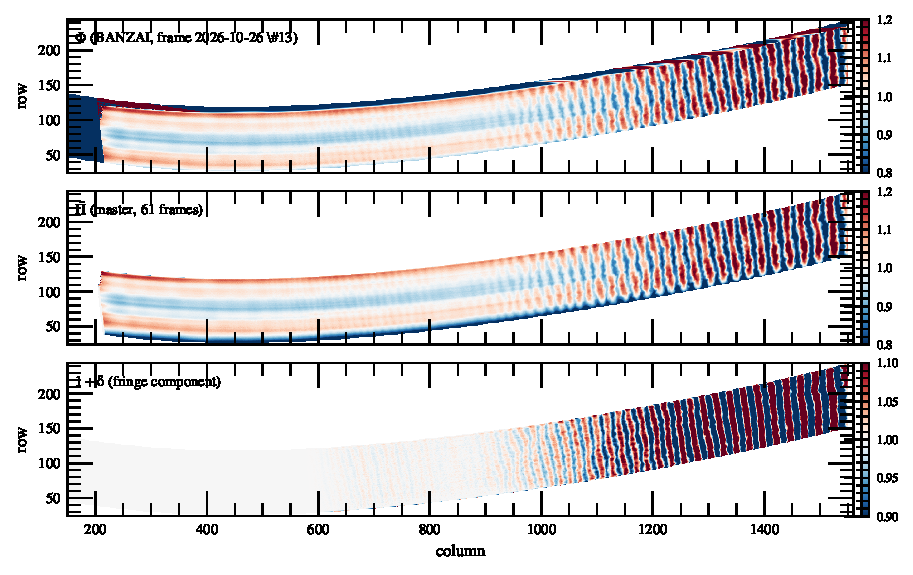
\includegraphics[width=\textwidth]{figures/fig_master.pdf}
\caption{Red order. Top: the map $\Phi$ the archive frame 2026-10-26 \#13 was divided by (shifted by $-8.9$ rows; note
the invalid edges). Middle: the master lamp pattern $\bar\Pi$ from the un-shifted maps of 61 frames. Bottom: its fringe
component $1+\delta$ (eq.~\ref{eq:delta}).}
\label{fig:master}
\end{figure}

\section{Fringe fit}
\label{sec:fringe_fit}
\textit{Shift.} To first order $R=R_0(1+a\,\delta)$ with $R_0$ smooth along the dispersion on fringe scales. With
$\mathcal{H}[\cdot]$ the residual from a 21-pixel running median along $x$, for every trial shift $(\Delta x,\Delta y)$
on a 0.5-pixel grid with $|\Delta x|,|\Delta y|\le2$,
\begin{equation}
\hat a=\frac{\sum w\,\mathcal{H}[R]\,\mathcal{H}[R\,\delta']}{\sum w\,\mathcal{H}[R\,\delta']^2},\qquad
\chi^2(\Delta x,\Delta y)=\sum w\left(\mathcal{H}[R]-\hat a\,\mathcal{H}[R\,\delta']\right)^2,
\label{eq:fringe2d}
\end{equation}
where $\delta'(x,y)=\delta(x-\Delta x,y-\Delta y)$, $w=1/\sigma_R^2$, and the sums run over the red-order pixels at
7000--9800\,\AA{} more than 6 rows from the slit ends. The minimum is well defined (period $\approx11$\,pixels in
$\Delta x$) and lies at $|\Delta x|\le1$, $|\Delta y|\le1$ for all frames.

\textit{Amplitude (initial model).} The 2-d fit under-corrects, so the correction is applied to the extracted spectrum. The profile-weighted fringe of each 1-pixel bin $\beta$ is
\begin{equation}
f_\beta=\frac{\sum_{i\in\beta}P_i\,\delta'_i}{\sum_{i\in\beta}P_i},
\label{eq:fringe1d}
\end{equation}
and the extracted counts are divided by $1+A(\lambda)f_\beta$, where the shift of $\delta'$ is the 2-d one.
The amplitude $A(\lambda)$ can be fitted freely on a spectrum by linear least squares of
$\mathcal{H}_{\rm 1d}[F]$ on $\mathcal{H}_{\rm 1d}[F\,f]$ ($\mathcal{H}_{\rm 1d}$: difference of 25\,\AA{} and 200\,\AA{}
running medians, telluric bands excluded) in a wavelength region. This is reliable on the smooth standards but not on
a single AGN spectrum, where it latches onto real structure. The amplitude is, however, very stable within one
instrument configuration, so it is calibrated per slit width as the median of the free fits over an ensemble of
frames, in four regions (6800--7500, 7500--8300, 8300--9100, 9100--9800\,\AA), and interpolated linearly between their
centres (Table~\ref{tab:amplaw}). Regions where the median is negative or its scatter exceeds half its value
(6800--7500\,\AA, where $\delta$ is still tapered in and most pixels are telluric) take the value of the nearest
reliable region. This uses no target information. The amplitude exceeds unity because the stored lamp map has a
diluted fringe contrast, and it differs between the 2 and 6\,arcsec slits, plausibly because slit-filling light reaches
each pixel over a wider wavelength range in a wide slit. This model is kept as an option
(\texttt{method='amplitude'}); Section~\ref{sec:fringe_harmonic} explains why it leaves $\approx5$ per cent
residuals and describes the default model.

\begin{table}
\centering
\caption{Fringe amplitude $A(\lambda)$ per slit width: median and robust scatter of the free fits over the ensemble of frames. $^{a}$Unreliable region (negative or scatter $>$ half the value); the value of the nearest reliable region is used.}
\label{tab:amplaw}
\begin{tabular}{lcccc}
\toprule
Slit & 7150\,\AA & 7900\,\AA & 8700\,\AA & 9450\,\AA \\
 & \multicolumn{4}{c}{($A$, no unit: multiplies the normalised fringe pattern)} \\
\midrule
6\,arcsec (50 frames) & \AmpSixA & \AmpSixB & \AmpSixC & \AmpSixD \\
2\,arcsec (18 frames) & \AmpTwoA & \AmpTwoB & \AmpTwoC & \AmpTwoD \\
\bottomrule
\end{tabular}
\end{table}



\section{Sky model}
\label{sec:sky}
For every 1-pixel wavelength bin $\beta$ of an order (\banzai{}'s binning, which follows the line tilt), the sky is a
polynomial along the slit,
\begin{equation}
S_\beta(y_{\rm o})=\sum_{k=0}^{2}b_{\beta k}\,y_{\rm o}^k,
\label{eq:sky}
\end{equation}
fitted by weighted least squares to the unmasked pixels with $|y_{\rm p}|>m\,\sigma_{\rm p}$ and
$|y_{\rm o}|<y_{\rm max}-6$, with iterative $3\sigma$ clipping. The mask half-width is $m=4$ unless that leaves fewer
than 25 per cent of the slit's pixels, in which case $m$ is reduced to the corresponding quantile of
$|y_{\rm p}|/\sigma_{\rm p}$ (but not below 2); the degree is reduced while fewer than $4(K+1)$ sky pixels remain, and set
to zero when all sky pixels lie on one side of the object. When the mask has been reduced, the sky pixels contain the
object's wings, so the sky polynomial and the object are fitted jointly to all slit pixels,
$R_i=\sum_k b_{\beta k}y_{{\rm o},i}^k+F'_\beta P_i$, with iterative clipping; only the sky part is kept. In synthetic
tests with $\sigma_{\rm p}=9$\,pixels in a 60-row slit this removes an 11 per cent flux bias. Its covariance
$C_\beta=(V^{\rm T}WV)^{-1}$ ($V$ the Vandermonde matrix, $W$ the inverse variances) is propagated into the
extraction errors. This replaces the 2-d spline sky of \banzai{} \citep{Kelson2003}, which cannot follow the
discontinuities introduced by the fringe map.

\section{Extraction}
\label{sec:extraction}
For bin $\beta$, with net counts $d_i=R_i-S_\beta(y_{{\rm o},i})$, profile weights $P_i$ (\banzai's fitted profile,
normalised to unit sum per column) and pixels within $|y_{\rm p}|<5\sigma_{\rm p}$, the optimal extraction
\citep{Horne1986} is
\begin{equation}
F_\beta=\frac{\sum_i a_i d_i}{\sum_i a_i P_i},\qquad a_i=\frac{P_i}{V_i},\qquad
V_i = r^2+\max(F_\beta P_i+S_{\beta,i},0),
\label{eq:horne}
\end{equation}
iterated with $V$ from the model (not the data); at each iteration the single pixel with the largest
$(d_i-F_\beta P_i)^2/V_i$ is rejected if this exceeds 25 (cosmic rays), up to $\max(2,\,0.1N_\beta)$ pixels per bin
(more ``outliers'' indicate a profile mismatch, not cosmic rays). The read noise is $r=3.5\,e^-$. Its variance is
\begin{equation}
\sigma^2_{F_\beta}=\frac{\sum_i a_i^2V_i+\mathbf{g}^{\rm T}C_\beta\,\mathbf{g}}{\left(\sum_i a_iP_i\right)^2},\qquad
\mathbf{g}=\sum_i a_i\,\mathbf{v}_i,
\label{eq:hornevar}
\end{equation}
with $\mathbf{v}_i=(y_{{\rm o},i}^2,y_{{\rm o},i},1)$ the sky basis at pixel $i$. A fixed-aperture extraction for RM is
\begin{equation}
F^{\rm box}_\beta=\frac{\sum_{|y_{\rm p}|<h}d_i}{\sum_{\rm all\ rows}P_i},
\label{eq:boxcarext}
\end{equation}
with $h=10$\,pixels ($\pm3.4$\,arcsec) by default; the denominator is the number of columns the bin spans, which
gives the same normalisation as \banzai{} for bins that collect 0, 1 or 2 pixels per row. In synthetic tests the
recovered fluxes are unbiased (optimal 2 per cent, boxcar 3 per cent including a cosmic ray on the trace) and the
normalised residuals have rms 1.03 (optimal) and 1.09 (boxcar).

\section{Results}
\label{sec:results_fringe}
Fig.~\ref{fig:edge} shows the frame region where the shifted lamp flat had destroyed the data; the stripes are gone
and the largest number of spikes in a spectrum drops from \SpMaxOld{} to \SpMaxNew. Fig.~\ref{fig:residuals} shows the
2-d residuals: in the bright-moon frame the robust rms of the normalised residuals at 7000--9500\,\AA{} drops from
1.70 to 1.44 in the sky rows and from 1.83 to 1.41 on the object; on the standard from 1.17 to 1.09 and 1.98 to 1.90.
In the dark frame the residuals are dominated by a mismatch of the (common) profile model and are unchanged (1.12 and
1.14 in the sky rows). Fig.~\ref{fig:fringe1d} compares extracted red orders. The fringe metric of the Fairall~9 spectra
drops from \FrOld{} to \FrNewOpt{} per cent and the fringing in the median spectrum from \FrMedOld{} to \FrMedNewOpt{}
per cent (Fig.~\ref{fig:series}); on the EG\,21 spectra from \EGfrOld{} to \EGfrNew{} per cent. This metric
smooths over 25\,\AA{} and includes real spectral structure and telluric residuals in its windows; the unsmoothed
comparison of Table~\ref{tab:fringevariants} isolates the fringe correction: the harmonic model halves the residual
of the amplitude law and comes within a factor $\approx2$ of the photon-noise floor (Fig.~\ref{fig:harmonic}). Because RM fits every
spectrum separately, Fig.~\ref{fig:individual} shows all spectra individually, divided by a power law: in the archive
products every spectrum carries 10--20 per cent fringes; after the correction the residual in the clean windows is
\IndivNewF{} per cent for Fairall~9 and \IndivNewE{} per cent for EG\,21 (\banzai: \IndivOldF{} and \IndivOldE), and no
periodic pattern is left in single spectra; the faintest spectra (signal-to-noise ratio 11--16 per pixel, 3--4\,arcsec
seeing) are photon-noise limited. The individual spectra also expose a feature that is \emph{not} a fringe residual:
a step of $\approx30$ per cent at $\approx9285$\,\AA{}, preceded by a bump in the gap between water bands at
9240--9285\,\AA, present in every version including the first one. Redward of 8900\,\AA{} there is no telluric-free
continuum: both the continuum used to measure the telluric transmission and the sensitivity correction are extrapolated
from shorter wavelengths, and the transmission is clipped to unity in the gap. The red end beyond 8900\,\AA{} is
therefore not yet reliably flux-calibrated (Chapter~\ref{sec:recommendations}). The residual in the A band also grows
with the width of the object's profile (Spearman $\rho=0.80$; 4 per cent for FWHM $<2.5$\,arcsec against 9 per cent
above, photon noise removed), because the telluric transmission measured on the 2\,arcsec standards is not matched to
the line-spread function of the 6\,arcsec spectra, which the seeing sets.

\begin{figure}[!htbp]
\centering
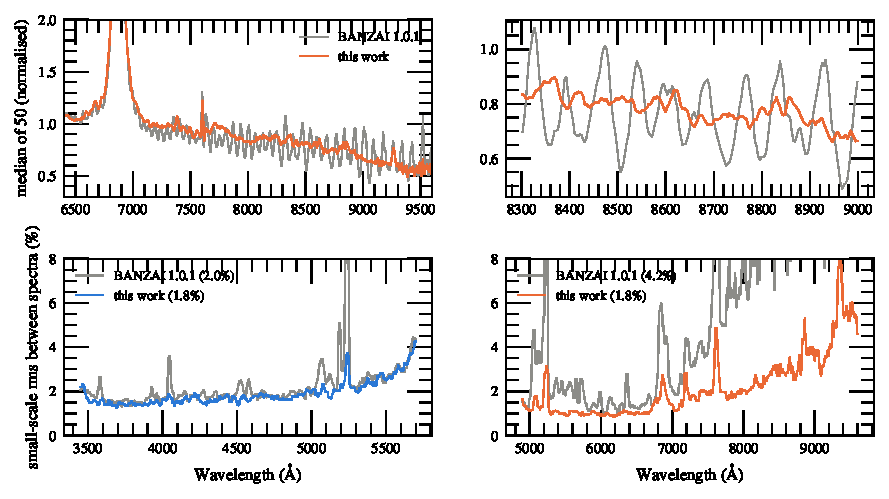
\includegraphics[width=\textwidth]{figures/fig_series.pdf}
\caption{Fairall~9, 50 spectra. Top: median red-order spectrum (left) and a zoom (right). Bottom: small-scale
($<200$\,\AA) scatter between the spectra, blue (left) and red (right) orders; archive in grey.}
\label{fig:series}
\end{figure}


\begin{figure}[!htbp]
\centering
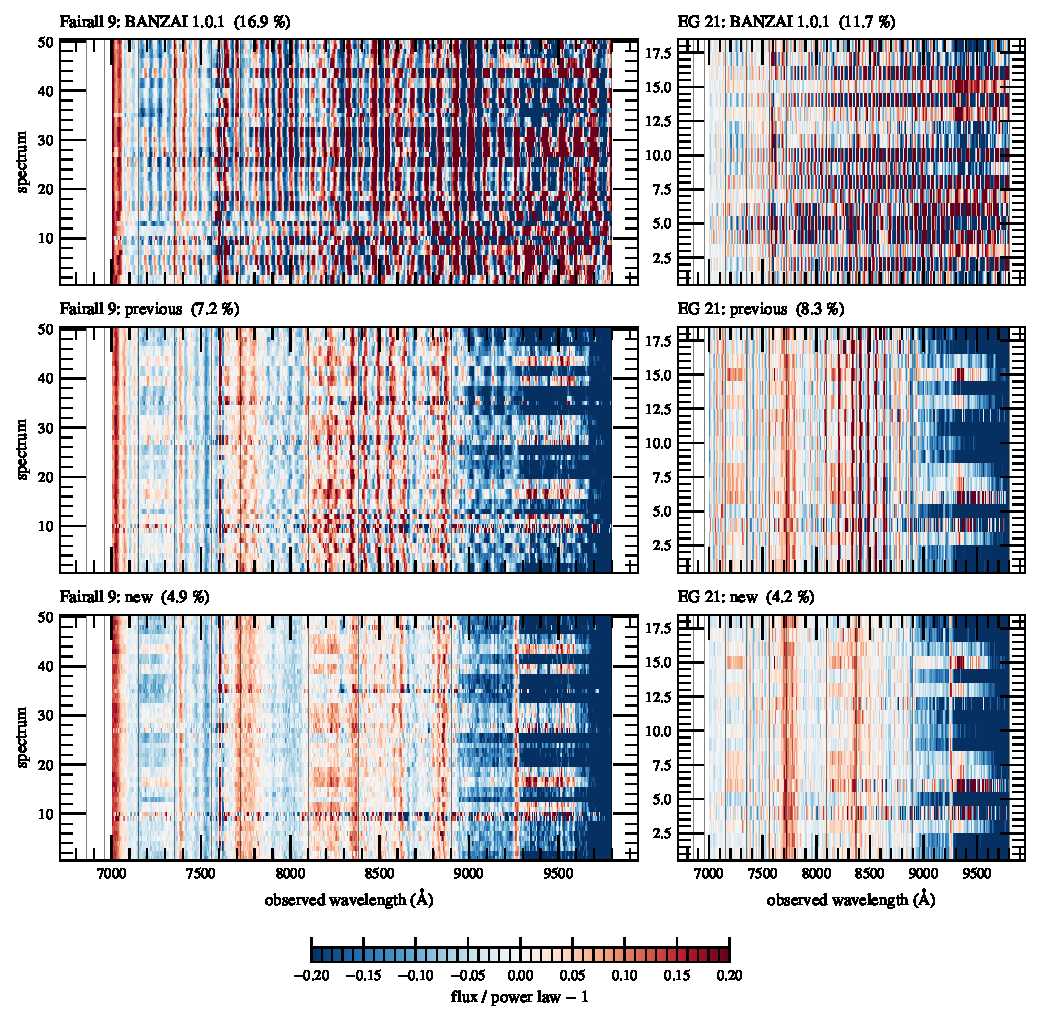
\includegraphics[width=\textwidth]{figures/fig_individual.pdf}
\caption{Individual flux-calibrated red-order spectra (one row per spectrum, in time order) divided by a power law
fitted at 7000--9800\,\AA{} outside the telluric bands (marked by vertical lines). Left: the 50 Fairall~9 spectra;
right: the 18 EG\,21 spectra. Top: \banzai{}~1.0.1; middle: initial model of the correction (lamp pattern times
amplitude law); bottom: this work (harmonic model, two passes). The number in each title is the median over spectra of
the rms in 7750--8050 and 8450--8900\,\AA. Remaining vertical structure is common to all spectra (broad lines of
Fairall~9, telluric residuals); horizontal bands beyond 9300\,\AA{} are night-to-night changes of the water-vapour
absorption.}
\label{fig:individual}
\end{figure}


\begin{figure}[!htbp]
\centering
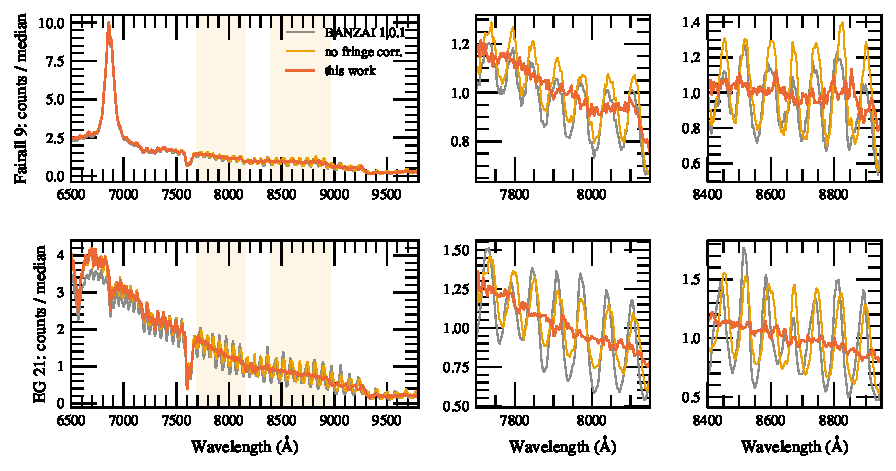
\includegraphics[width=\textwidth]{figures/fig_fringe1d.pdf}
\caption{Extracted red order (counts, normalised) of a Fairall~9 frame and an EG\,21 frame: archive (grey), fringe
division undone without new correction (yellow), this work (orange). The zooms are free of telluric bands.}
\label{fig:fringe1d}
\end{figure}


\begin{figure}[!htbp]
\centering
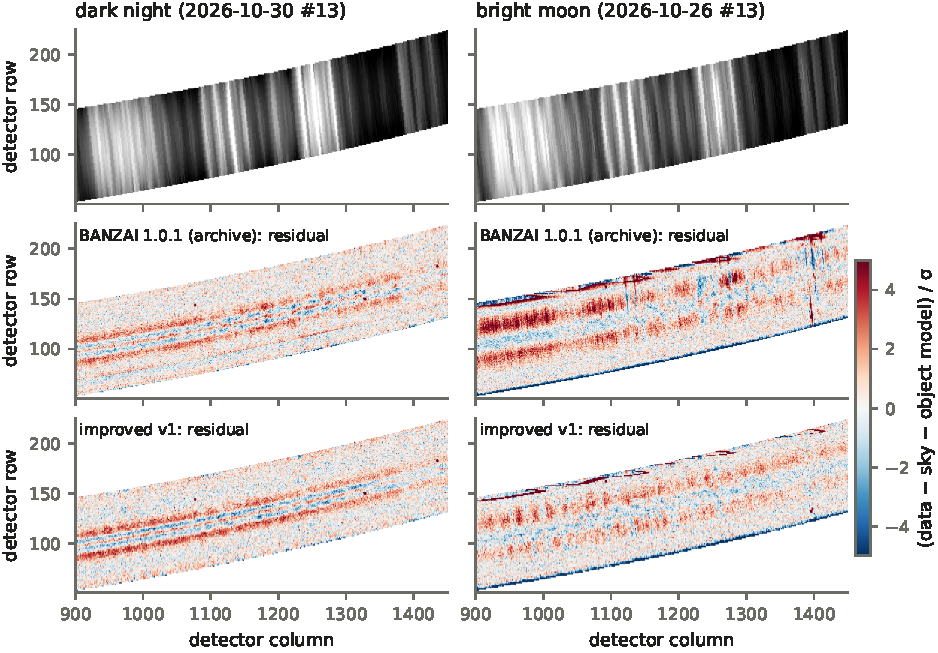
\includegraphics[width=\textwidth]{figures/fig_residuals.pdf}
\caption{Red order at $\approx7600$--9300\,\AA. Top: new sky model. Middle and bottom: normalised residuals (data $-$
sky $-$ profile $\times$ extracted flux)$/\sigma$ of the archive products and of this work, for a dark and a bright-moon
frame.}
\label{fig:residuals}
\end{figure}


The pixel-to-pixel scatter of the extractions agrees with the propagated uncertainties (ratio 0.8--1.2 in both
orders, before and after), so the extraction noise is photon-limited; the red order has the higher signal-to-noise
ratio (93--116 per 1-pixel bin at 4700--6800\,\AA{} against 39--76 in the blue). The ``noise'' of the red order in
the archive products was produced by the fringe correction and the sensitivity function, not by the extraction.
Optimal and fixed-aperture extractions perform alike on the small-scale metrics; the fixed aperture gives a more
consistent red/blue [O\,{\sc iii}] ratio (\FRBBox{} against \FRBOpt{} per cent), as expected for an extended
narrow-line region.


\chapter{Installing and running the improved pipeline}
\label{sec:app_install}
The improved pipeline (improved v3) is the \texttt{rm-improvements} branch of the fork
\url{https://github.com/Alymantara/banzai-floyds}; the full guide is \texttt{docs/INSTALL\_RM.md} in that branch.
Two problems were met when installing it on an Apple-silicon laptop, and both are avoided below.

\section{Environment}
\banzai{} needs PyTorch $\ge2.3$, for which there are no wheels for an Intel (x86\_64) Python running under Rosetta:
the environment must be native arm64, i.e.
\begin{verbatim}
python -c "import platform; print(platform.machine())"
\end{verbatim}
must print \texttt{arm64}. With conda, even from an Intel Anaconda:
\begin{verbatim}
git clone https://github.com/Alymantara/banzai-floyds.git
git -C banzai-floyds checkout rm-improvements
CONDA_SUBDIR=osx-arm64 conda create -y -p ./env-banzai python=3.12 pip
\end{verbatim}
On Linux any Python 3.10--3.12 virtual environment works.

\section{Installation}
\texttt{lco-banzai} compiles C extensions, and compiler settings exported by the login profile (here from an Intel
conda / oneAPI installation) made the build fail (\texttt{This is not the Intel oneAPI compiler};
\texttt{unsupported tapi file type ... for architecture x86\_64}). Installing, and running, from a clean environment
with the system compiler avoids it. A wrapper script \texttt{benv} next to the checkout does this (in zsh the command
cannot be kept in a variable, which zsh does not split into words):
\begin{verbatim}
#!/bin/sh
exec env -i HOME="$HOME" \
  PATH="$(cd "$(dirname "$0")" && pwd)/env-banzai/bin:/usr/bin:/bin:/usr/sbin:/sbin" \
  OPENTSDB_PYTHON_METRICS_TEST_MODE=True CC=/usr/bin/clang CXX=/usr/bin/clang++ \
  ${DB_ADDRESS:+DB_ADDRESS="$DB_ADDRESS"} "$@"
\end{verbatim}
\begin{verbatim}
chmod +x benv
./benv python -m pip install -e ./banzai-floyds
cd banzai-floyds && ../benv python -m pytest banzai_floyds/tests \
    --deselect banzai_floyds/tests/test_e2e.py        # 176 passed
\end{verbatim}
\texttt{OPENTSDB\_PYTHON\_METRICS\_TEST\_MODE} stops \banzai{} from sending metrics; the end-to-end tests need LCO's
test database.

\section{Reducing raw frames}
\begin{verbatim}
DB=sqlite:///$PWD/floyds.db
./benv banzai_floyds_offline setup-db --db-address $DB
./benv banzai_floyds_offline skyflats --db-address $DB \
       --raw-dir skyflats/ --processed-dir processed/
./benv banzai_floyds_offline chain --db-address $DB \
       --raw-dir raw/ --processed-dir processed/
\end{verbatim}
\texttt{setup-db} creates the calibration database (both FLOYDS sites, order locations, line-spread parameters, flux
standards). \texttt{skyflats} processes the sky flats listed in \texttt{data/orders/skyflats.dat}, which fix the shape
of the orders. \texttt{chain} classifies the raw frames from their headers and runs, in order: arcs, lamp flats, the
fringe phase masters (one per slit width and $\approx60$-d window), the standards, the residual fringe templates, the
standards again and the science frames (Section~\ref{sec:visit_timing} for the time per visit). The spectra are in
\texttt{processed/<site>/<camera>/<date>/processed/*-1d.fits.fz}; use the rows with \texttt{mask == 0} (bit 2 marks
the O$_2$ A band in science spectra). Keep more than 10\,GB of disk free: \banzai{} memory-maps its arrays in the
temporary directory and a processed 2-d frame is $\approx50$\,MB before it is made lean
(Section~\ref{sec:sites_disk}). Sky flats can be the raw frames or the processed \texttt{-f91} files from the archive
(for OGG only the 2019 March 29 set is listed). Both sites have an object-trace template and priors; for a new
instrument or after an intervention, rebuild them from the standards with \texttt{work/scripts/build\_trace\_template.py}
(without a template the pipeline falls back to the 1.1.0 polynomial). Flux standards must be in
\texttt{data/standards} to be used as standards; others are reduced as science.

\chapter{Line groups and telluric bands}
\label{app:tables}

\begin{table}
\centering
\caption{Arc line groups used for the refit (air wavelengths, \AA). Lines in one group share the shift $s_g$.
$\delta_g$ is the extra systematic error of unresolved blends. ``New'': not used by \banzai{}~1.0.1.}
\label{tab:groups}
\begin{tabular}{llcc}
\toprule
Order & Lines (\AA) & $\delta_g$ (\AA) & New \\
\midrule
blue & Hg 3650.158, 3654.842, 3663.279 & 0.5 & \\
blue & Hg 4046.565, 4077.837 & -- & \\
blue & Hg 4339.223, 4347.500, 4358.335 & 0.3 & \\
blue & Hg 4916.068 & -- & yes \\
blue & Hg 5460.750 & -- & \\
blue & Hg 5769.610, 5790.670 & -- & \\
red & Hg 4916.068 & -- & yes \\
red & Hg 5460.750 & -- & \\
red & Hg 5769.610, 5790.670 & -- & \\
red & Ar 6416.307 & -- & yes \\
red & Ar 6677.282 & -- & yes \\
red & Ar 6752.834, 6766.612 & -- & yes \\
red & Ar 6871.289, 6937.664, 6965.431 & 0.5 & \\
red & Ar 7067.218; 7147.042; 7272.936; 7383.980 & -- & \\
red & Ar 7503.869, 7514.652 & 1.0 & \\
red & Ar 7635.106; 7723.760+7724.207 (merged) & -- & \\
red & Ar 7948.176, 8006.157, 8014.786 & 0.5 & \\
red & Ar 8103.693, 8115.311 & 1.0 & \\
red & Ar 8264.522 & -- & \\
red & Ar 8408.210, 8424.647 & 1.0 & \\
red & Ar 8521.442; 8667.944; 9122.967 & -- & \\
red & Ar 9224.499; 9657.786; 9784.503 & -- & \\
\bottomrule
\end{tabular}
\end{table}

\begin{table}
\centering
\caption{Telluric bands used for the object zero point. $o_b$ is the band's offset relative to the A band
(median of 18 EG\,21 spectra after the arc refit); $\omega_b$ its weight in eq.~(\ref{eq:tellcomb}).}
\label{tab:bands}
\begin{tabular}{lccc}
\toprule
Band & Window (\AA) & $o_b$ (\AA) & $\omega_b$ \\
\midrule
O$_2$ A & 7550--7720 & 0 & 1 \\
H$_2$O & 7150--7350 & $+5.05$ & 0.5 \\
O$_2$ B & 6840--6960 & $+0.56$ & 0.5 \\
H$_2$O & 9250--9700 & $+0.53$ & 0.25 \\
\bottomrule
\end{tabular}
\end{table}


\end{document}
